\section{Fit results}
\label{ref:fit:results}

The pre-control fit is listed in \cref{appx:suppl:fit-pre-ctrl}.
The control fit results are plotted in
\cref{fig:ctrl-1os-d0,fig:ctrl-2os-d0,fig:ctrl-dd-d0} for \Dz channel;
\cref{fig:ctrl-1os-dst,fig:ctrl-2os-dst,fig:ctrl-dd-dst} for \Dstar channel.
The signal fit results are shown in
\cref{fig:sig-d0,fig:sig-dst}.
The fitted yield in the signal fit is reported in TAB.


\begin{figure}[htb]
    \centering
    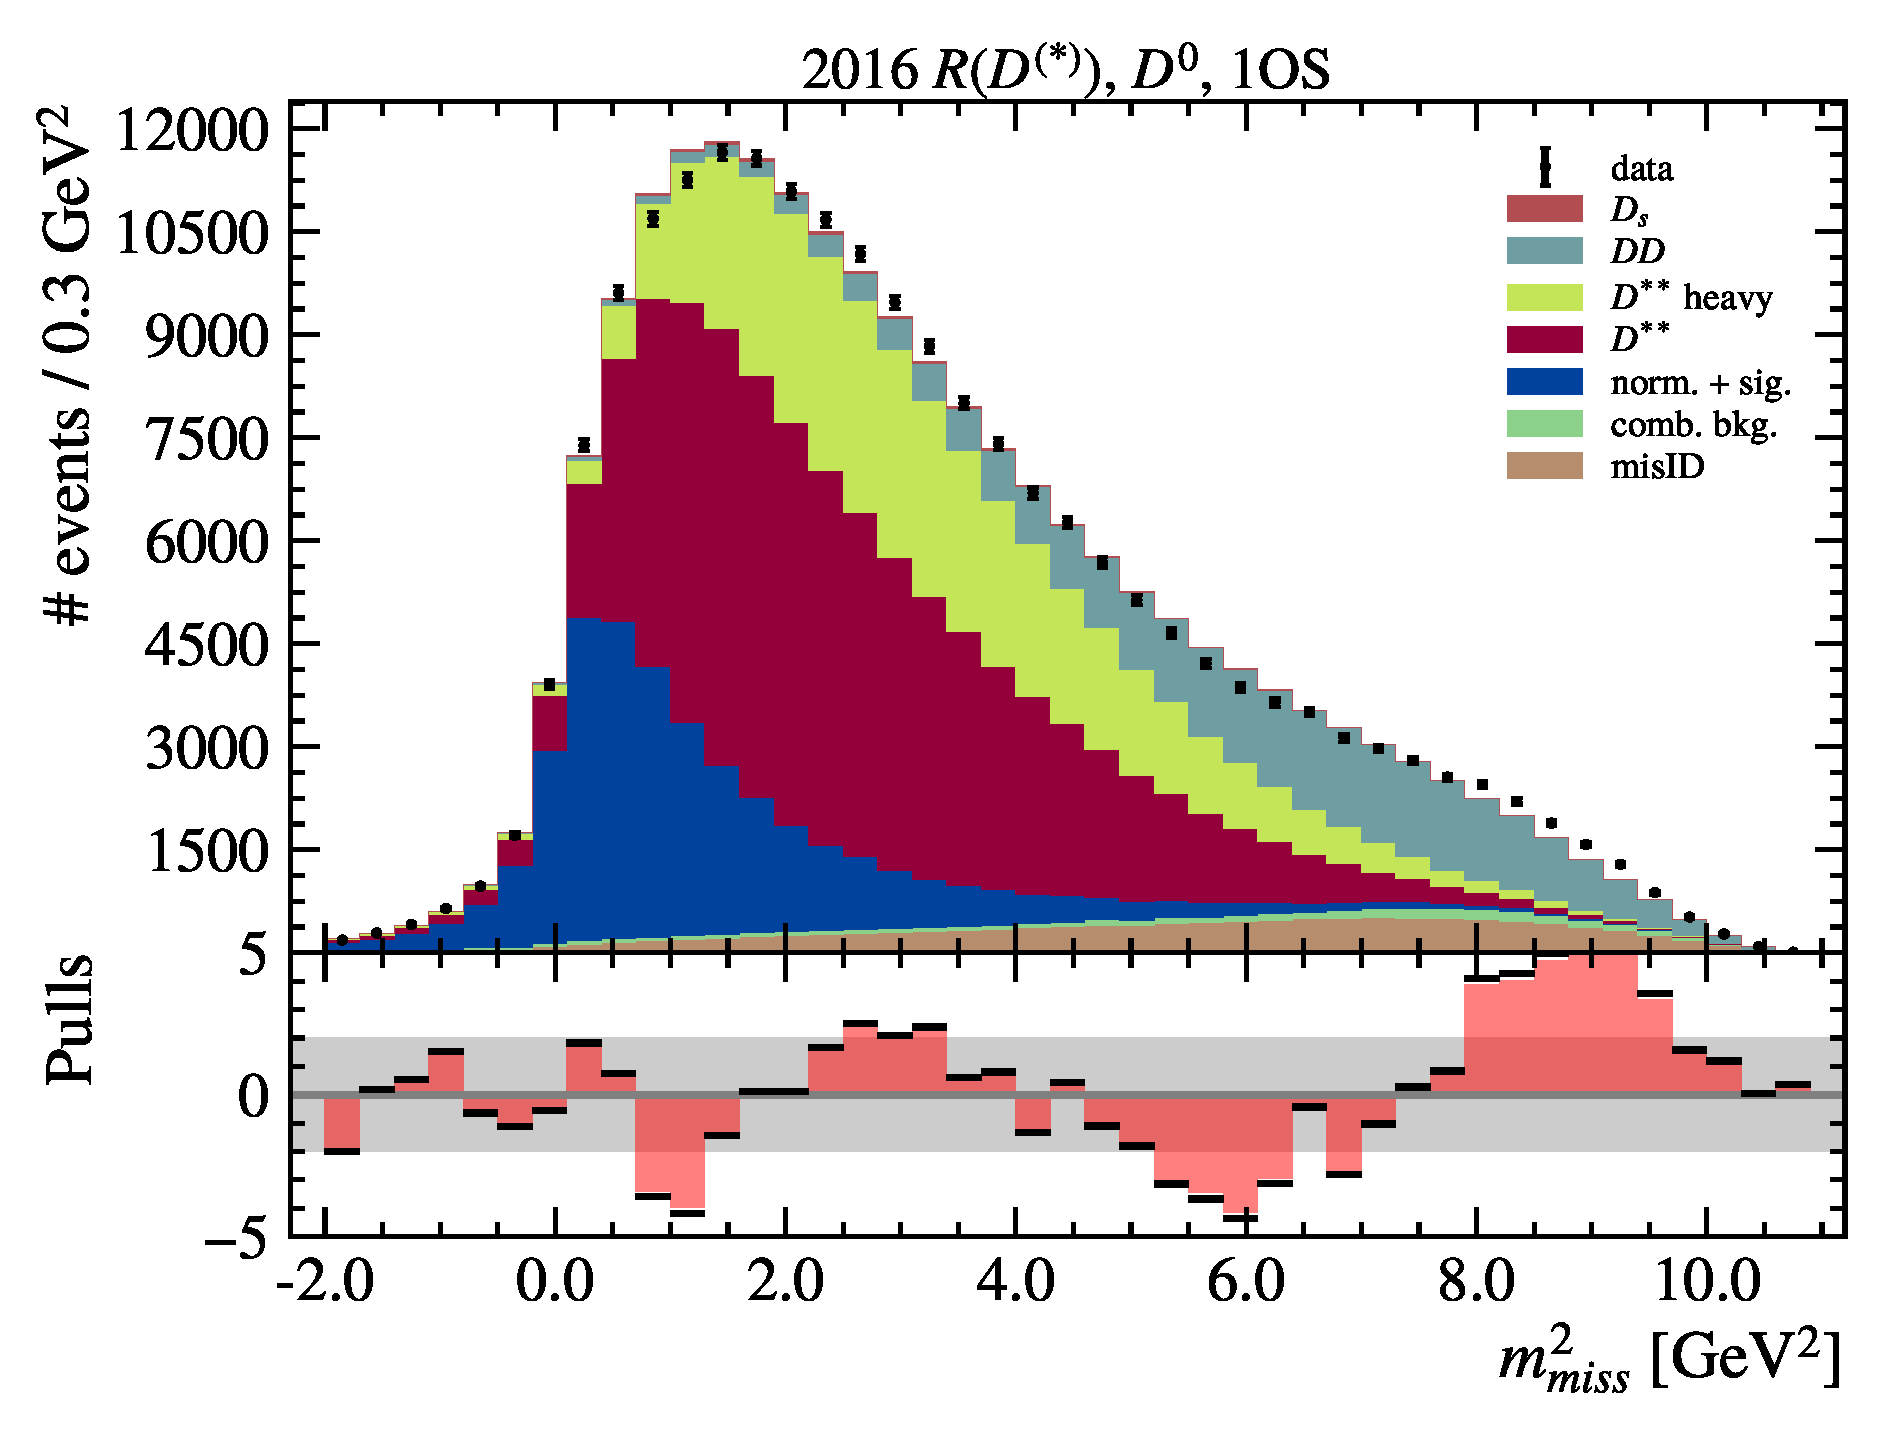
\includegraphics[width=0.32\textwidth]{./figs-fit-to-data/ctrl-fit/stacked/fit_result-stacked-D0-1os-mmiss2.pdf}
    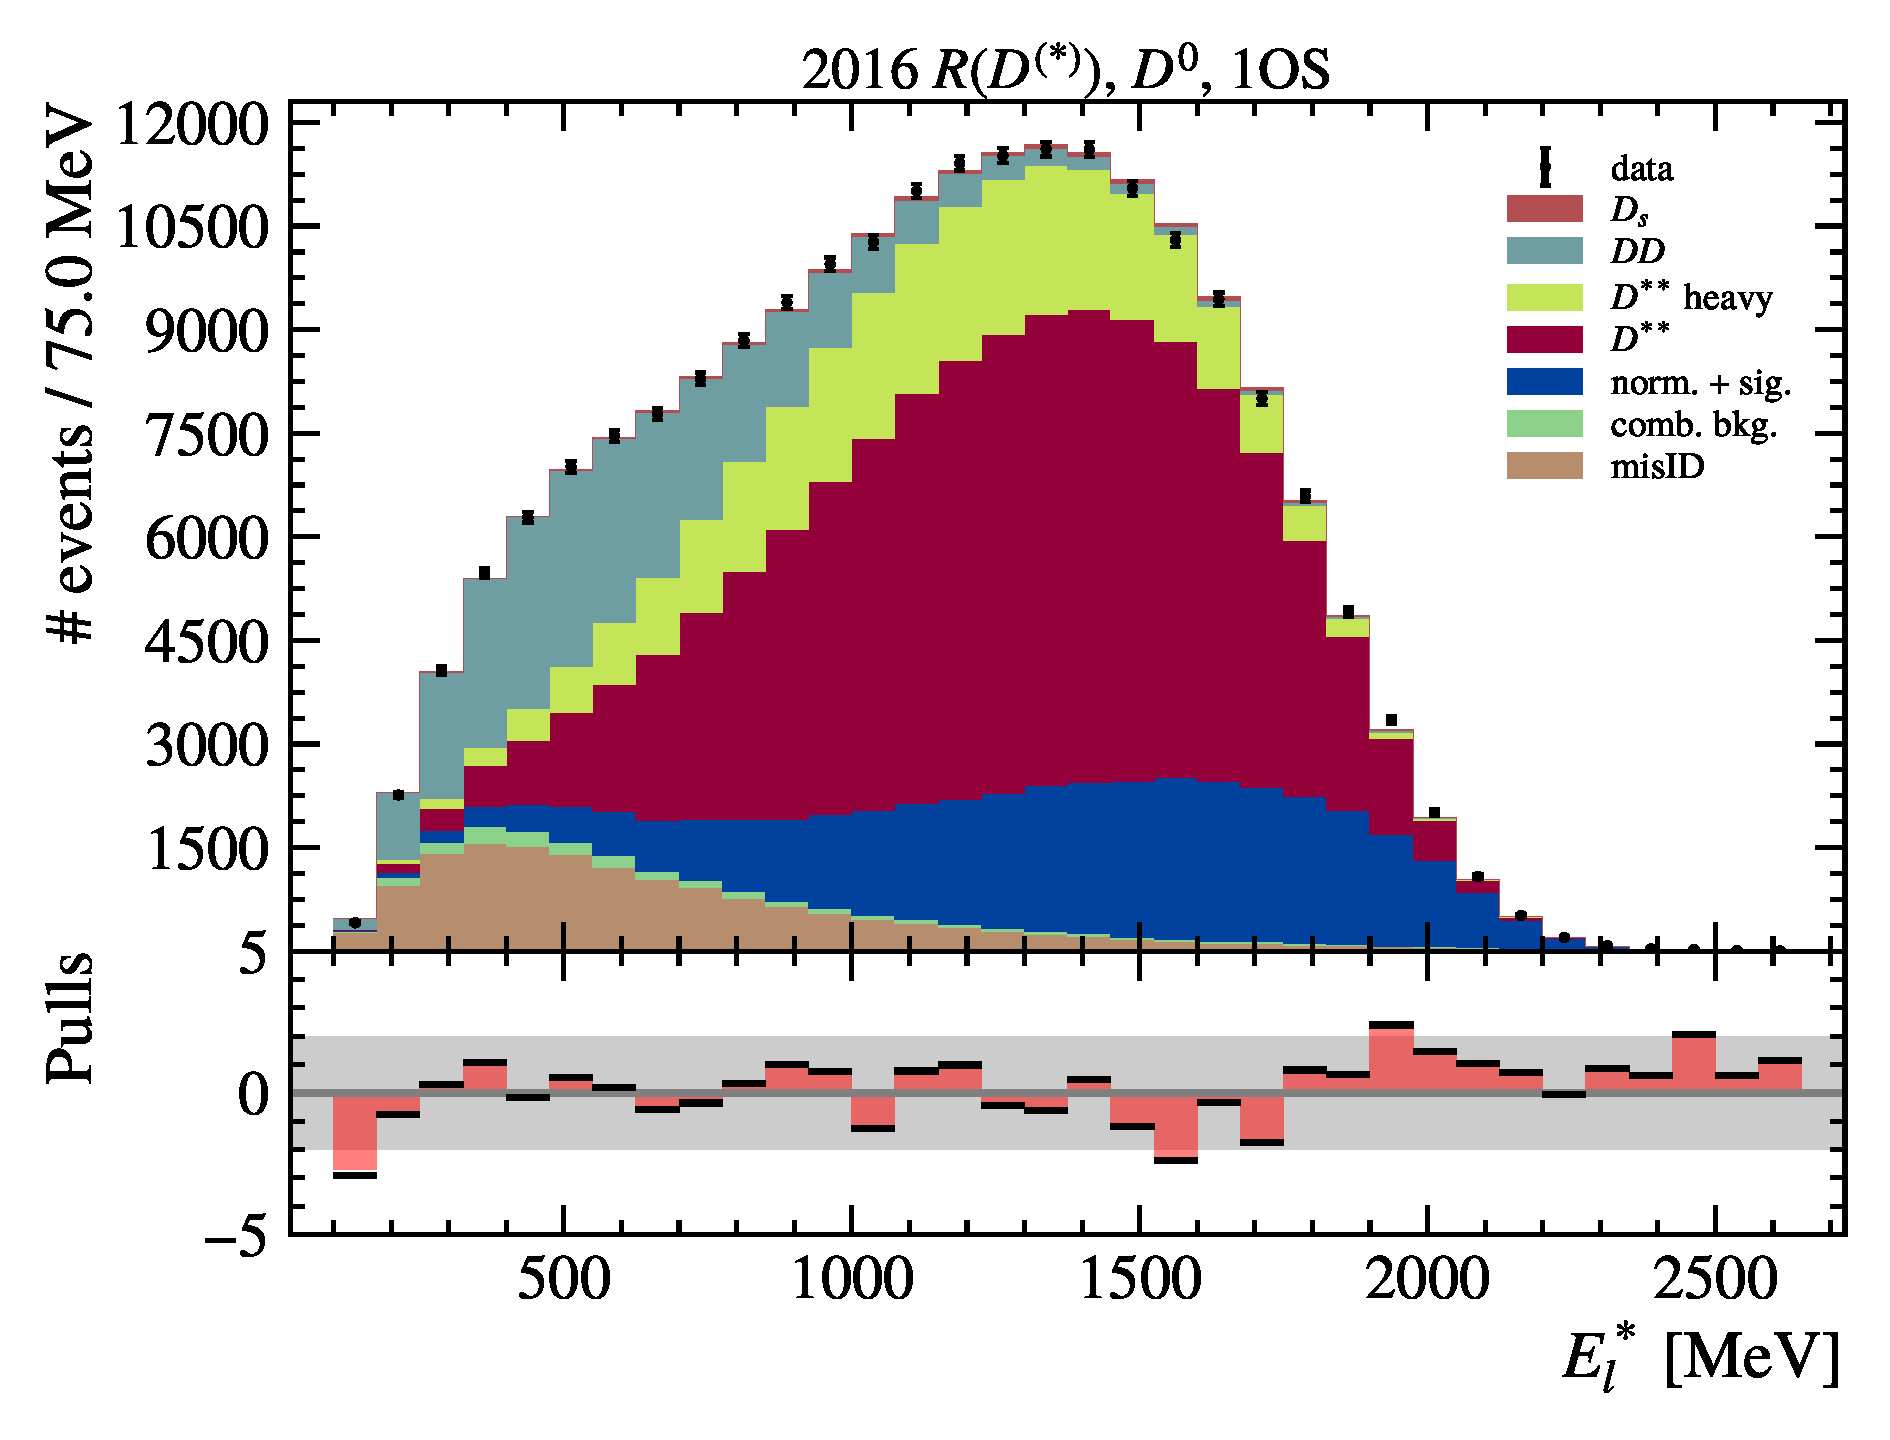
\includegraphics[width=0.32\textwidth]{./figs-fit-to-data/ctrl-fit/stacked/fit_result-stacked-D0-1os-el.pdf}
    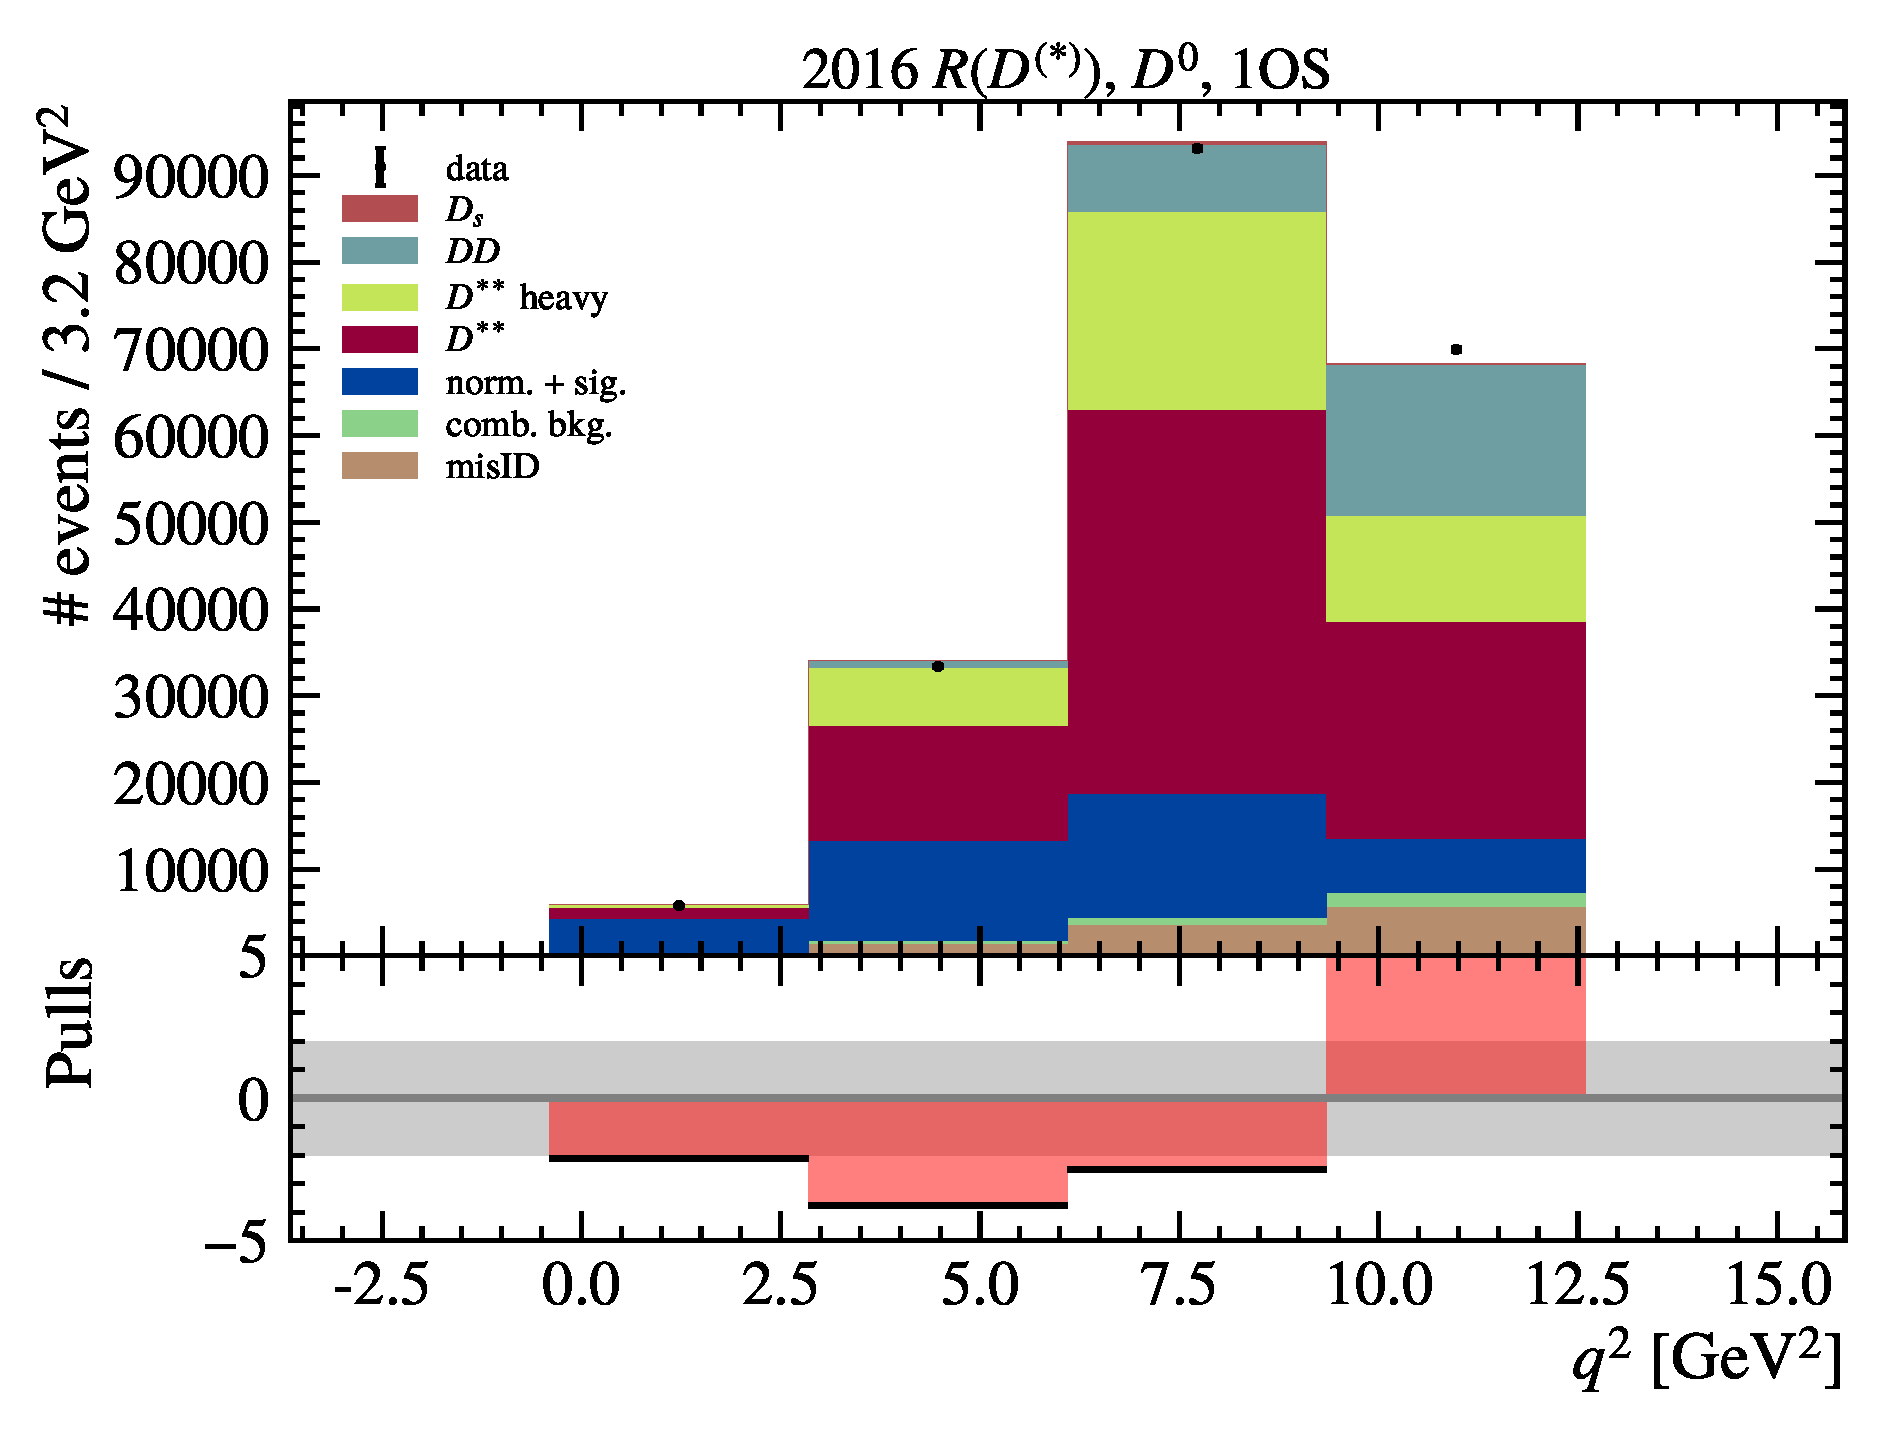
\includegraphics[width=0.32\textwidth]{./figs-fit-to-data/ctrl-fit/stacked/fit_result-stacked-D0-1os-q2.pdf}

    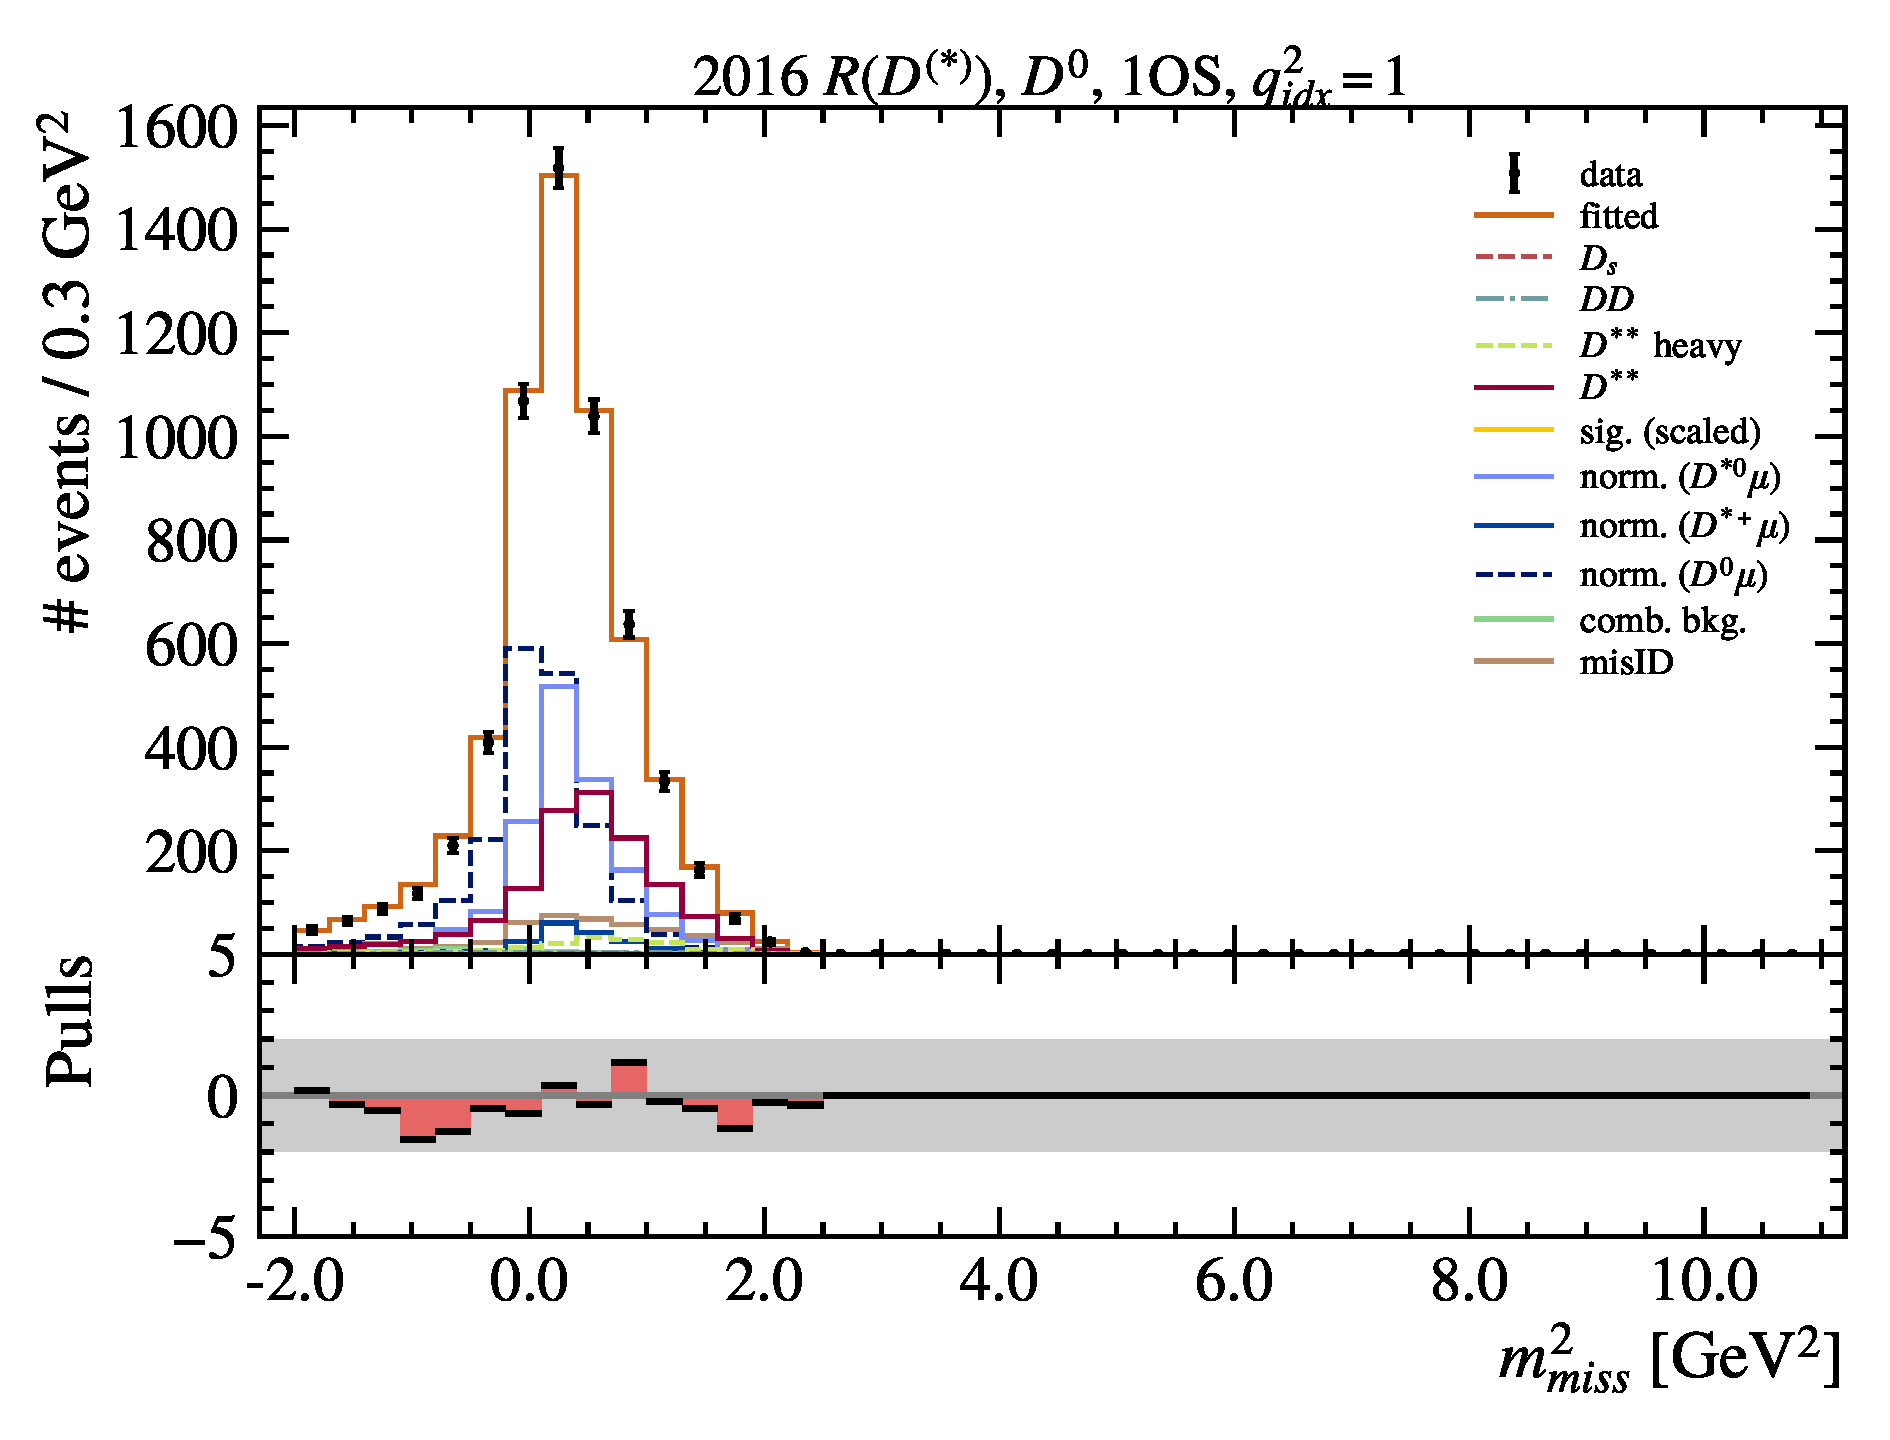
\includegraphics[width=0.24\textwidth]{./figs-fit-to-data/ctrl-fit/lines_q2_slices/fit_result-lines_q2_idx1-D0-1os-mmiss2.pdf}
    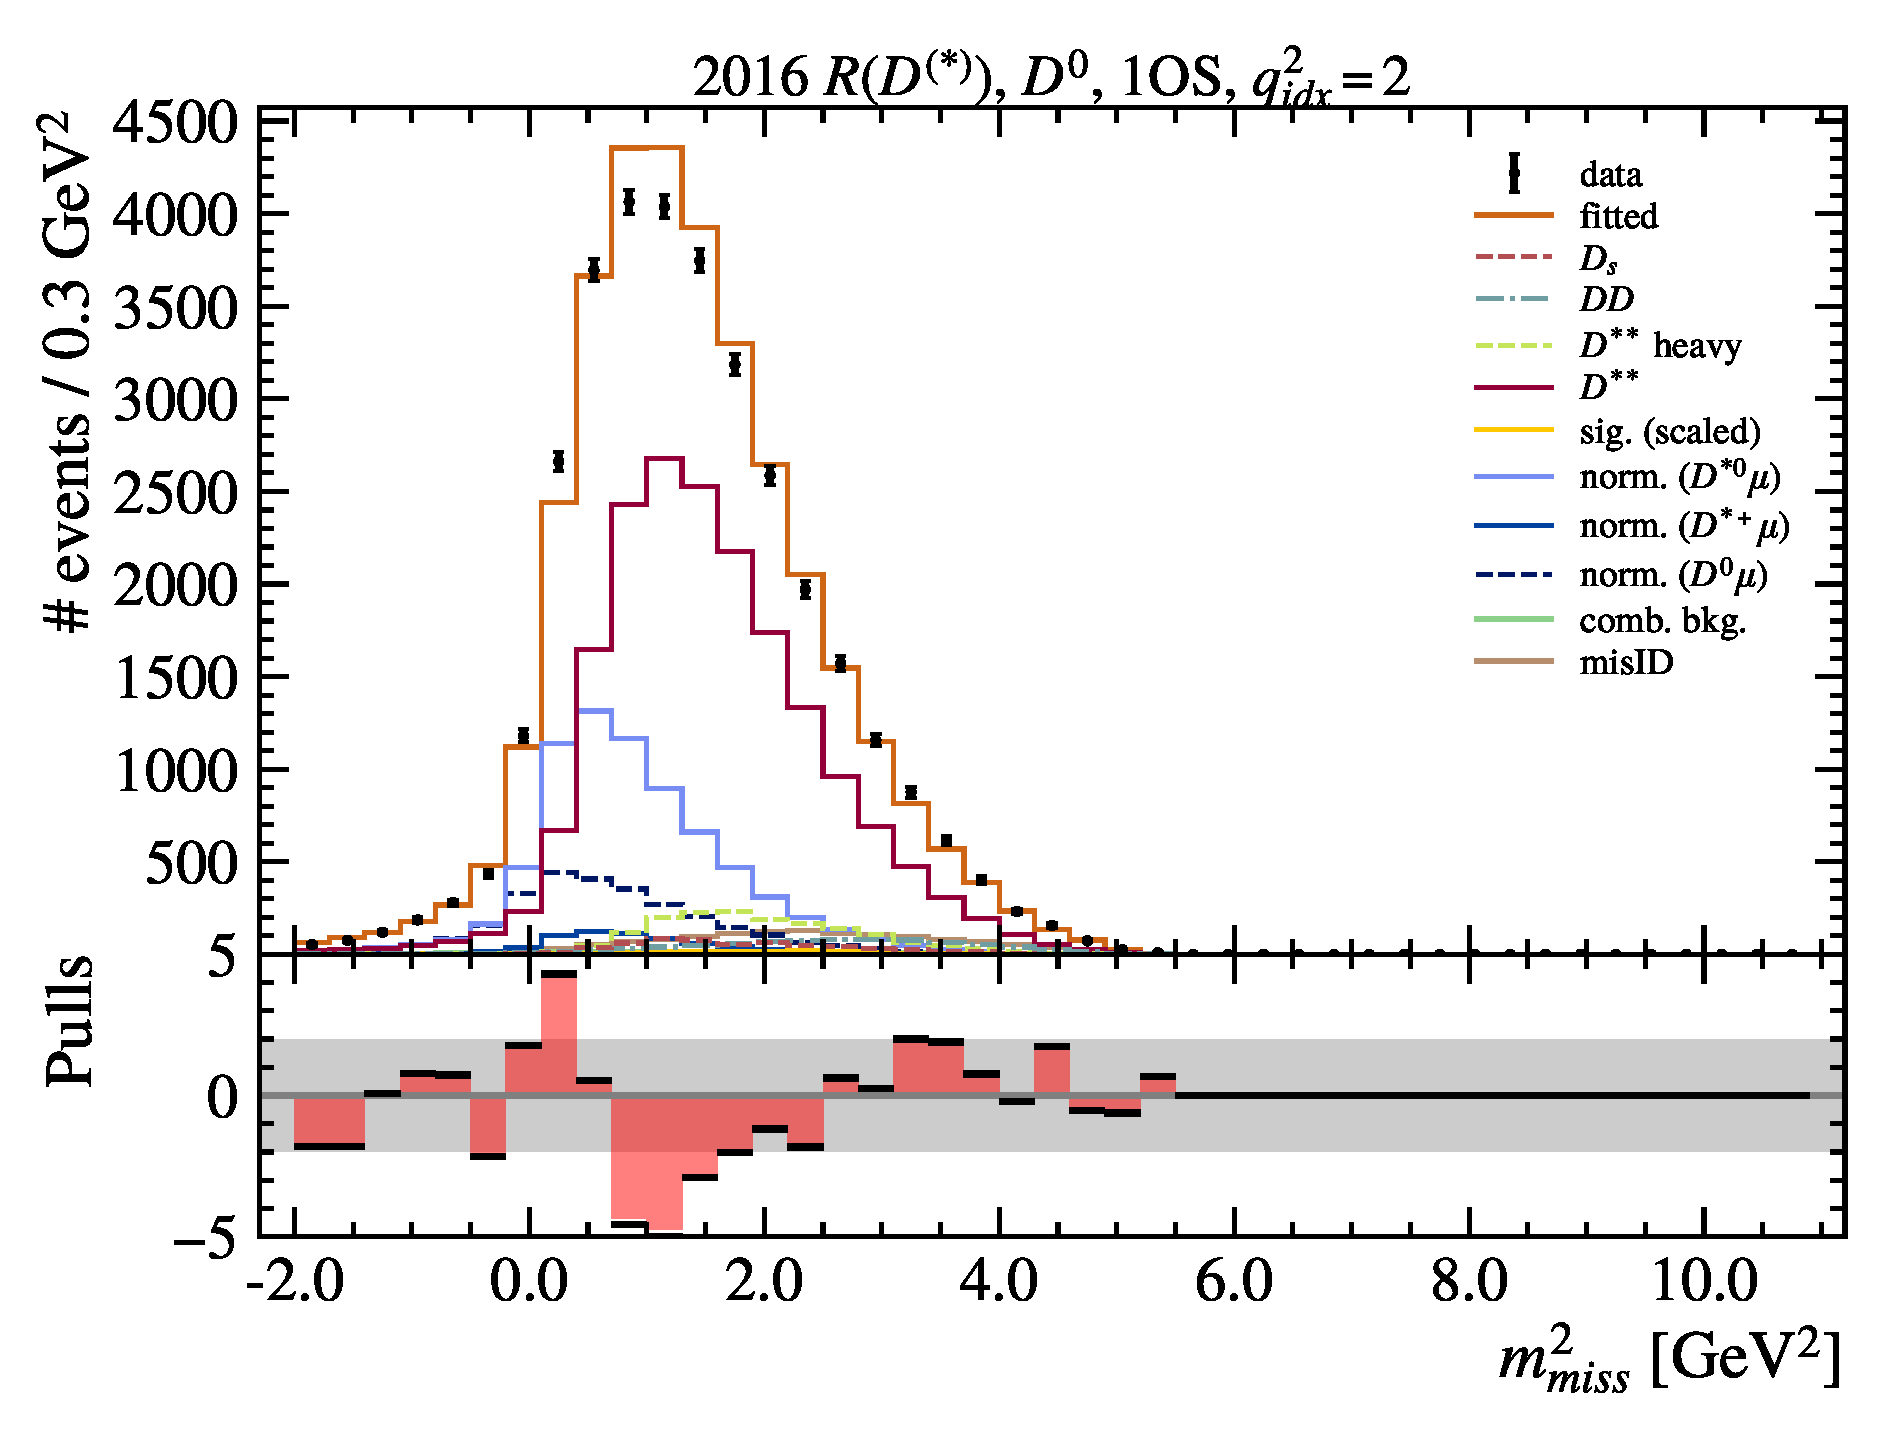
\includegraphics[width=0.24\textwidth]{./figs-fit-to-data/ctrl-fit/lines_q2_slices/fit_result-lines_q2_idx2-D0-1os-mmiss2.pdf}
    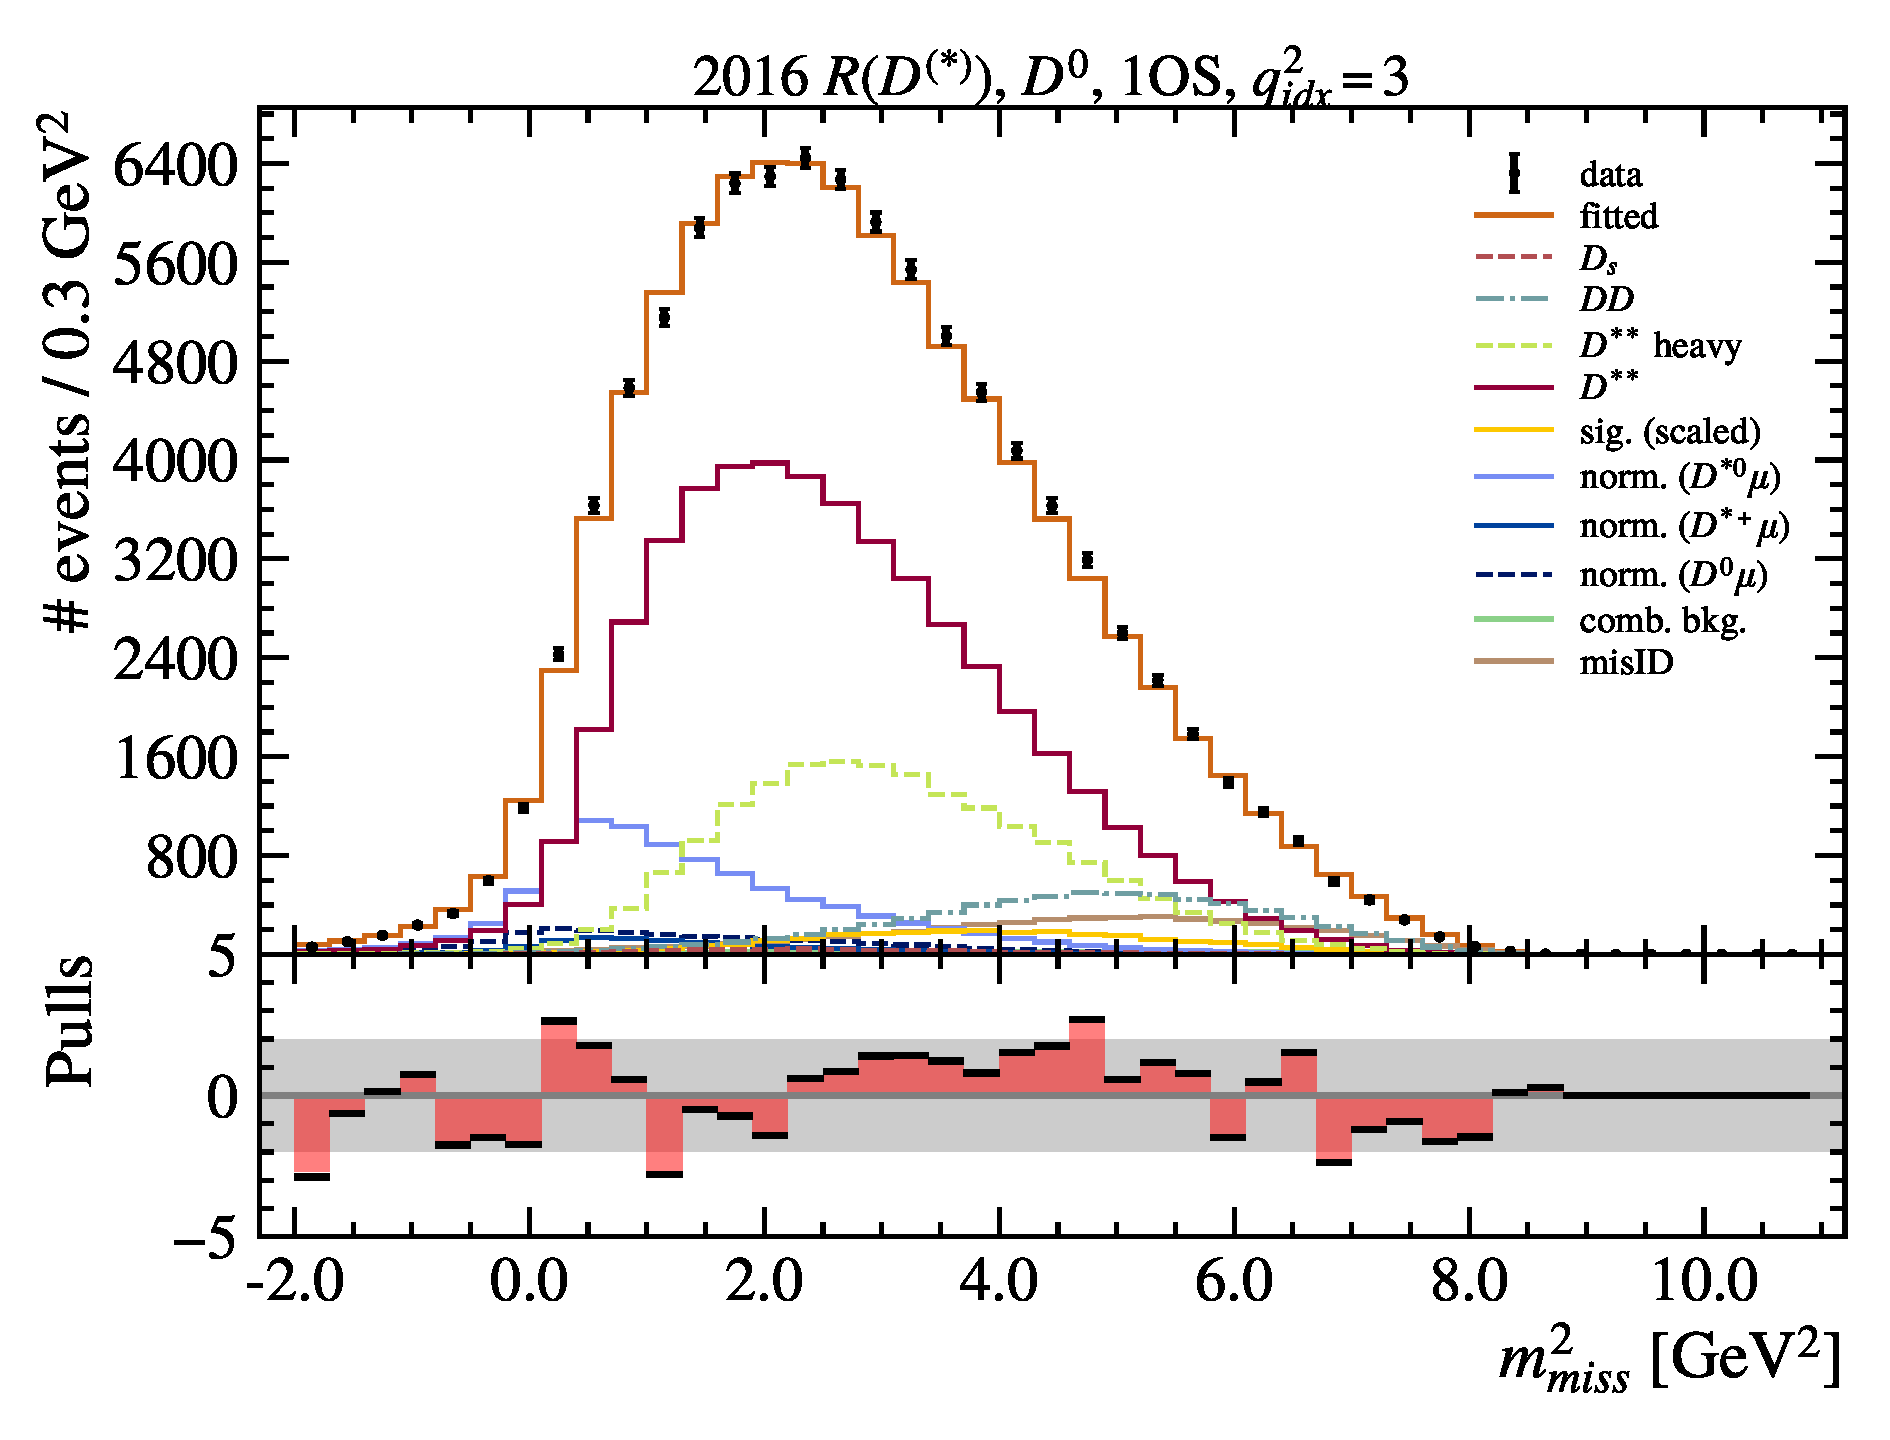
\includegraphics[width=0.24\textwidth]{./figs-fit-to-data/ctrl-fit/lines_q2_slices/fit_result-lines_q2_idx3-D0-1os-mmiss2.pdf}
    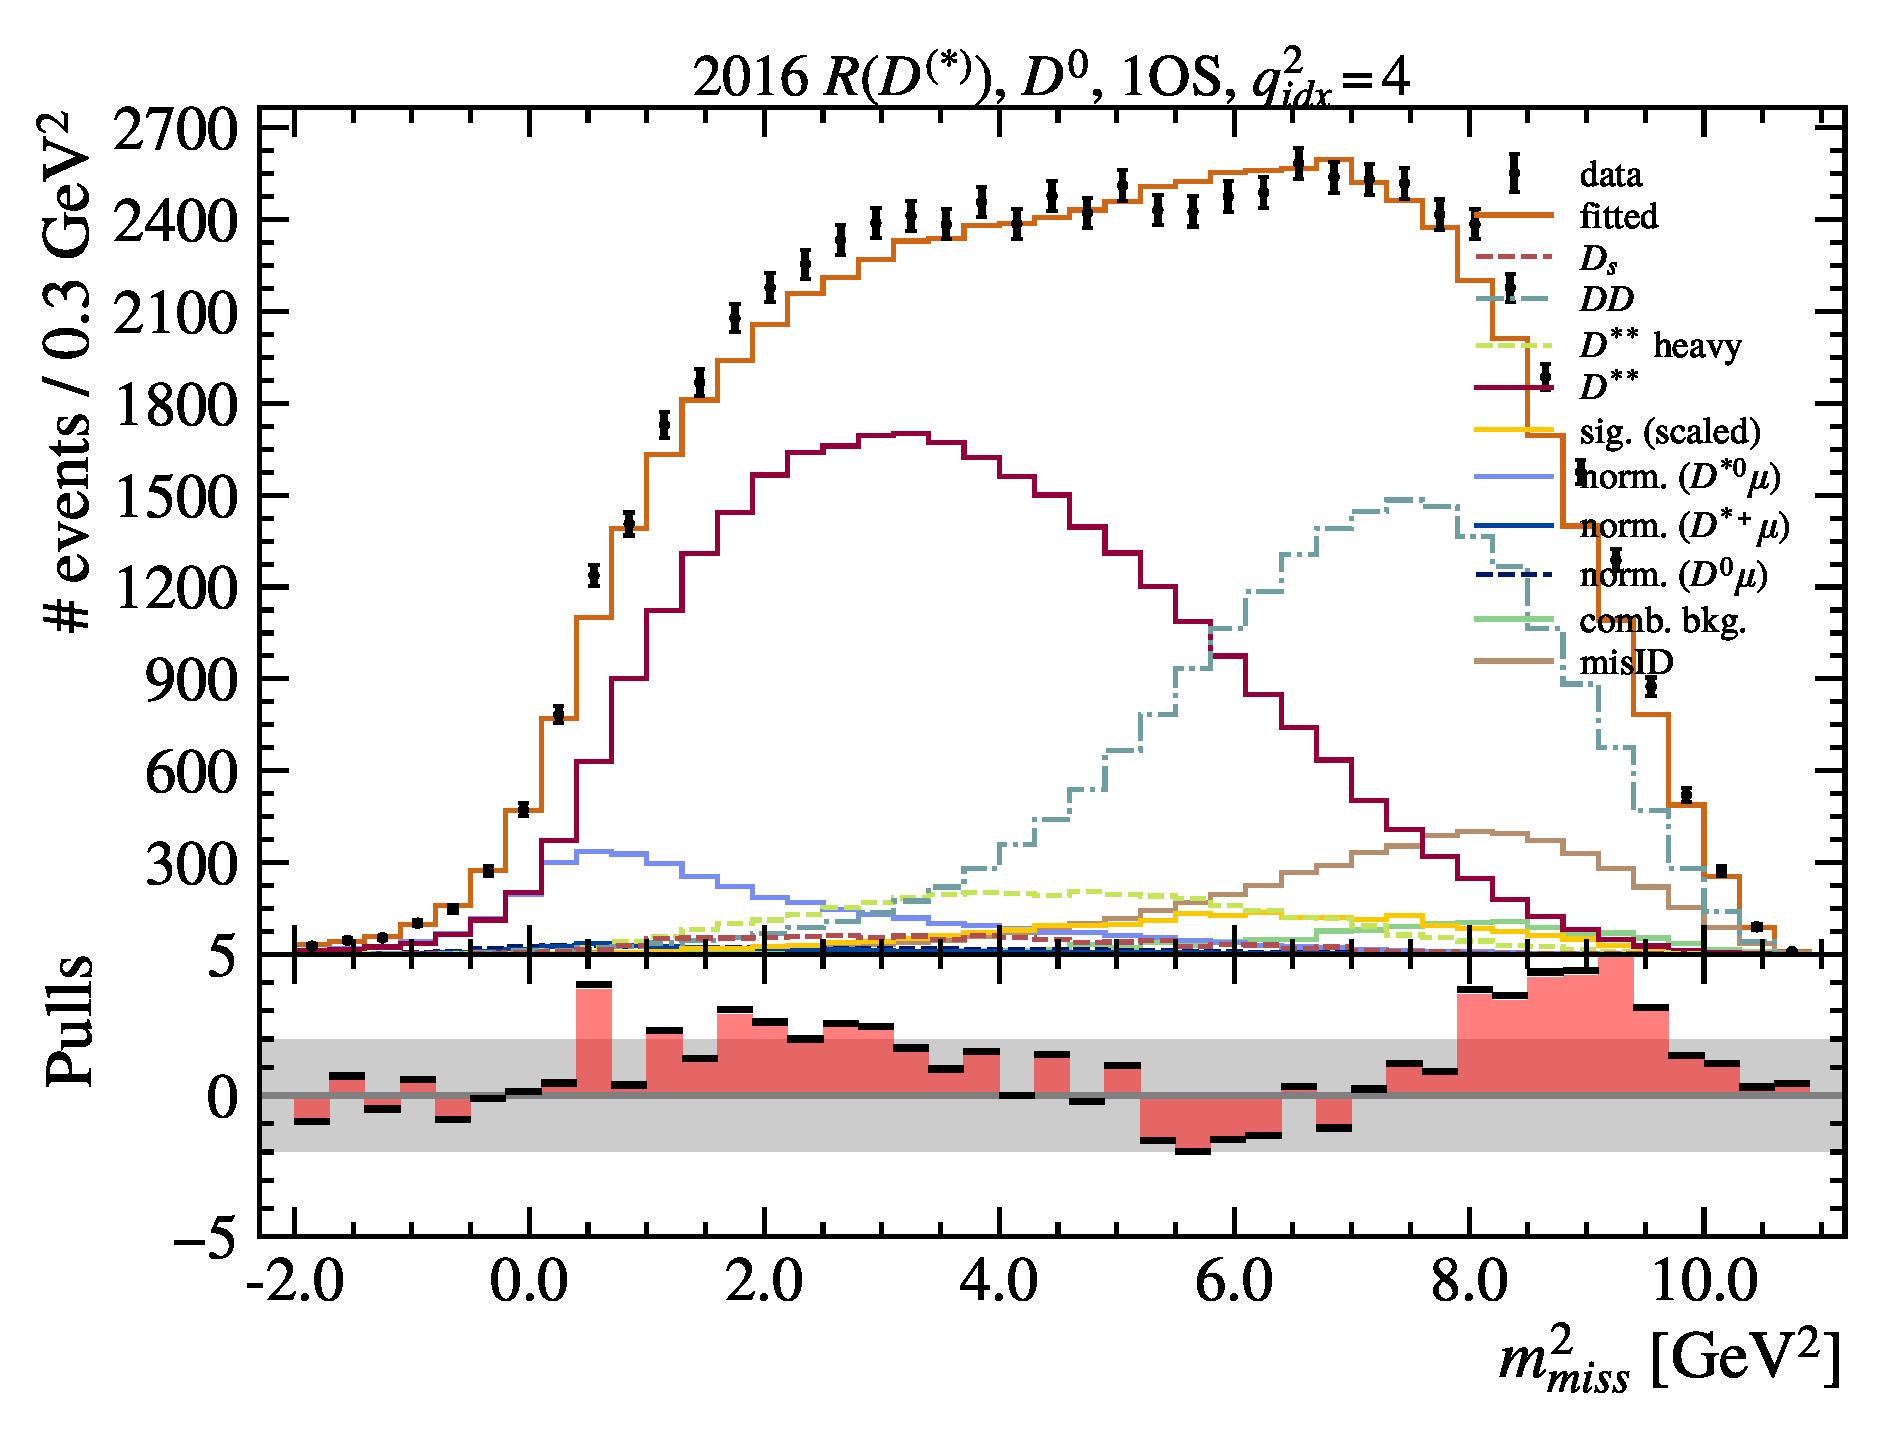
\includegraphics[width=0.24\textwidth]{./figs-fit-to-data/ctrl-fit/lines_q2_slices/fit_result-lines_q2_idx4-D0-1os-mmiss2.pdf}

    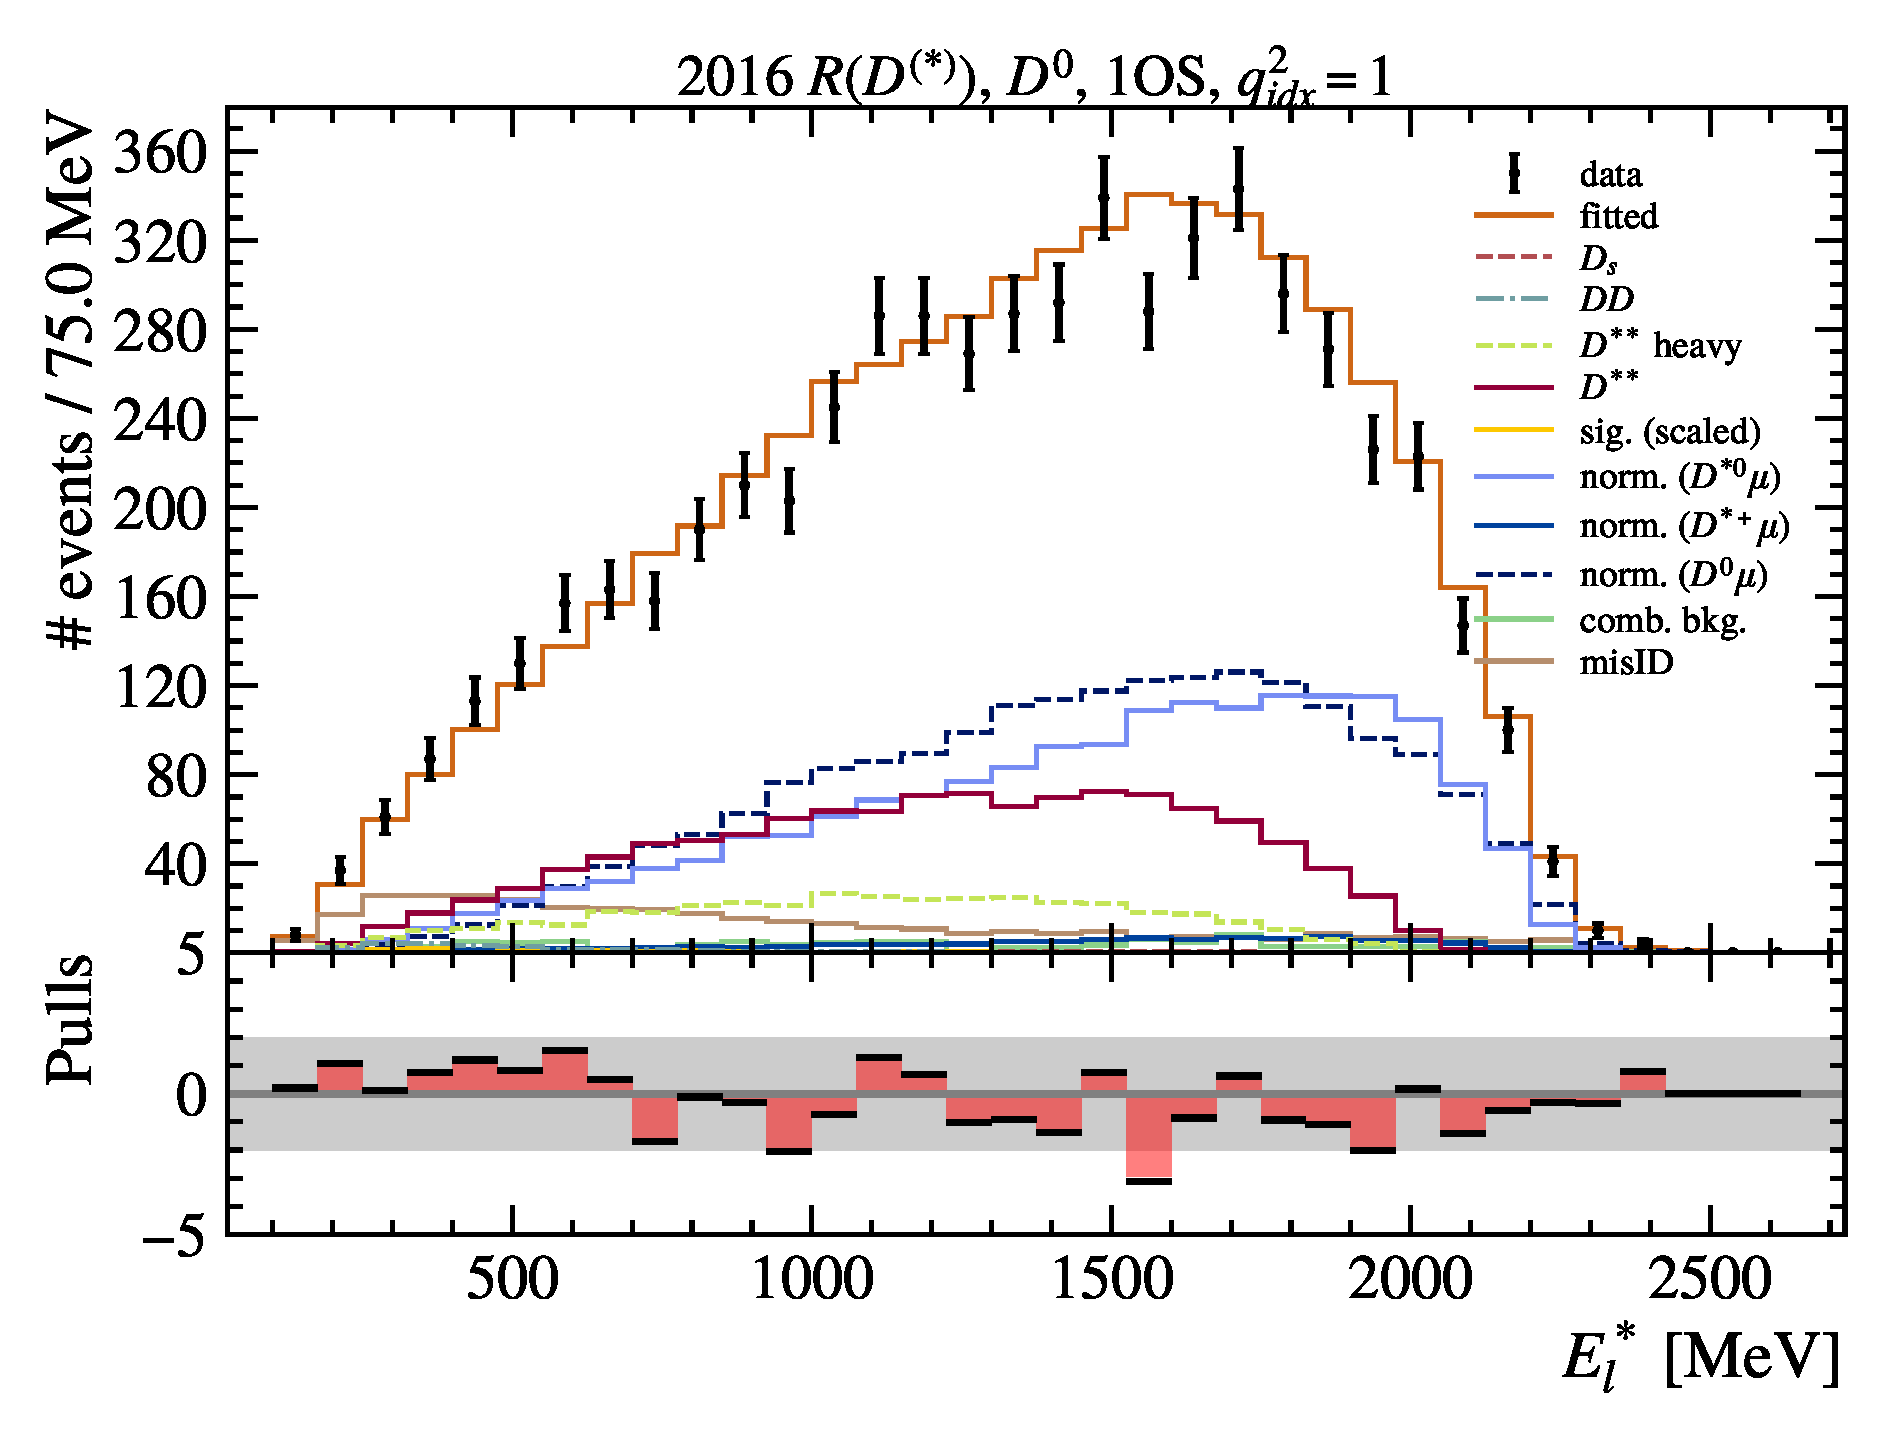
\includegraphics[width=0.24\textwidth]{./figs-fit-to-data/ctrl-fit/lines_q2_slices/fit_result-lines_q2_idx1-D0-1os-el.pdf}
    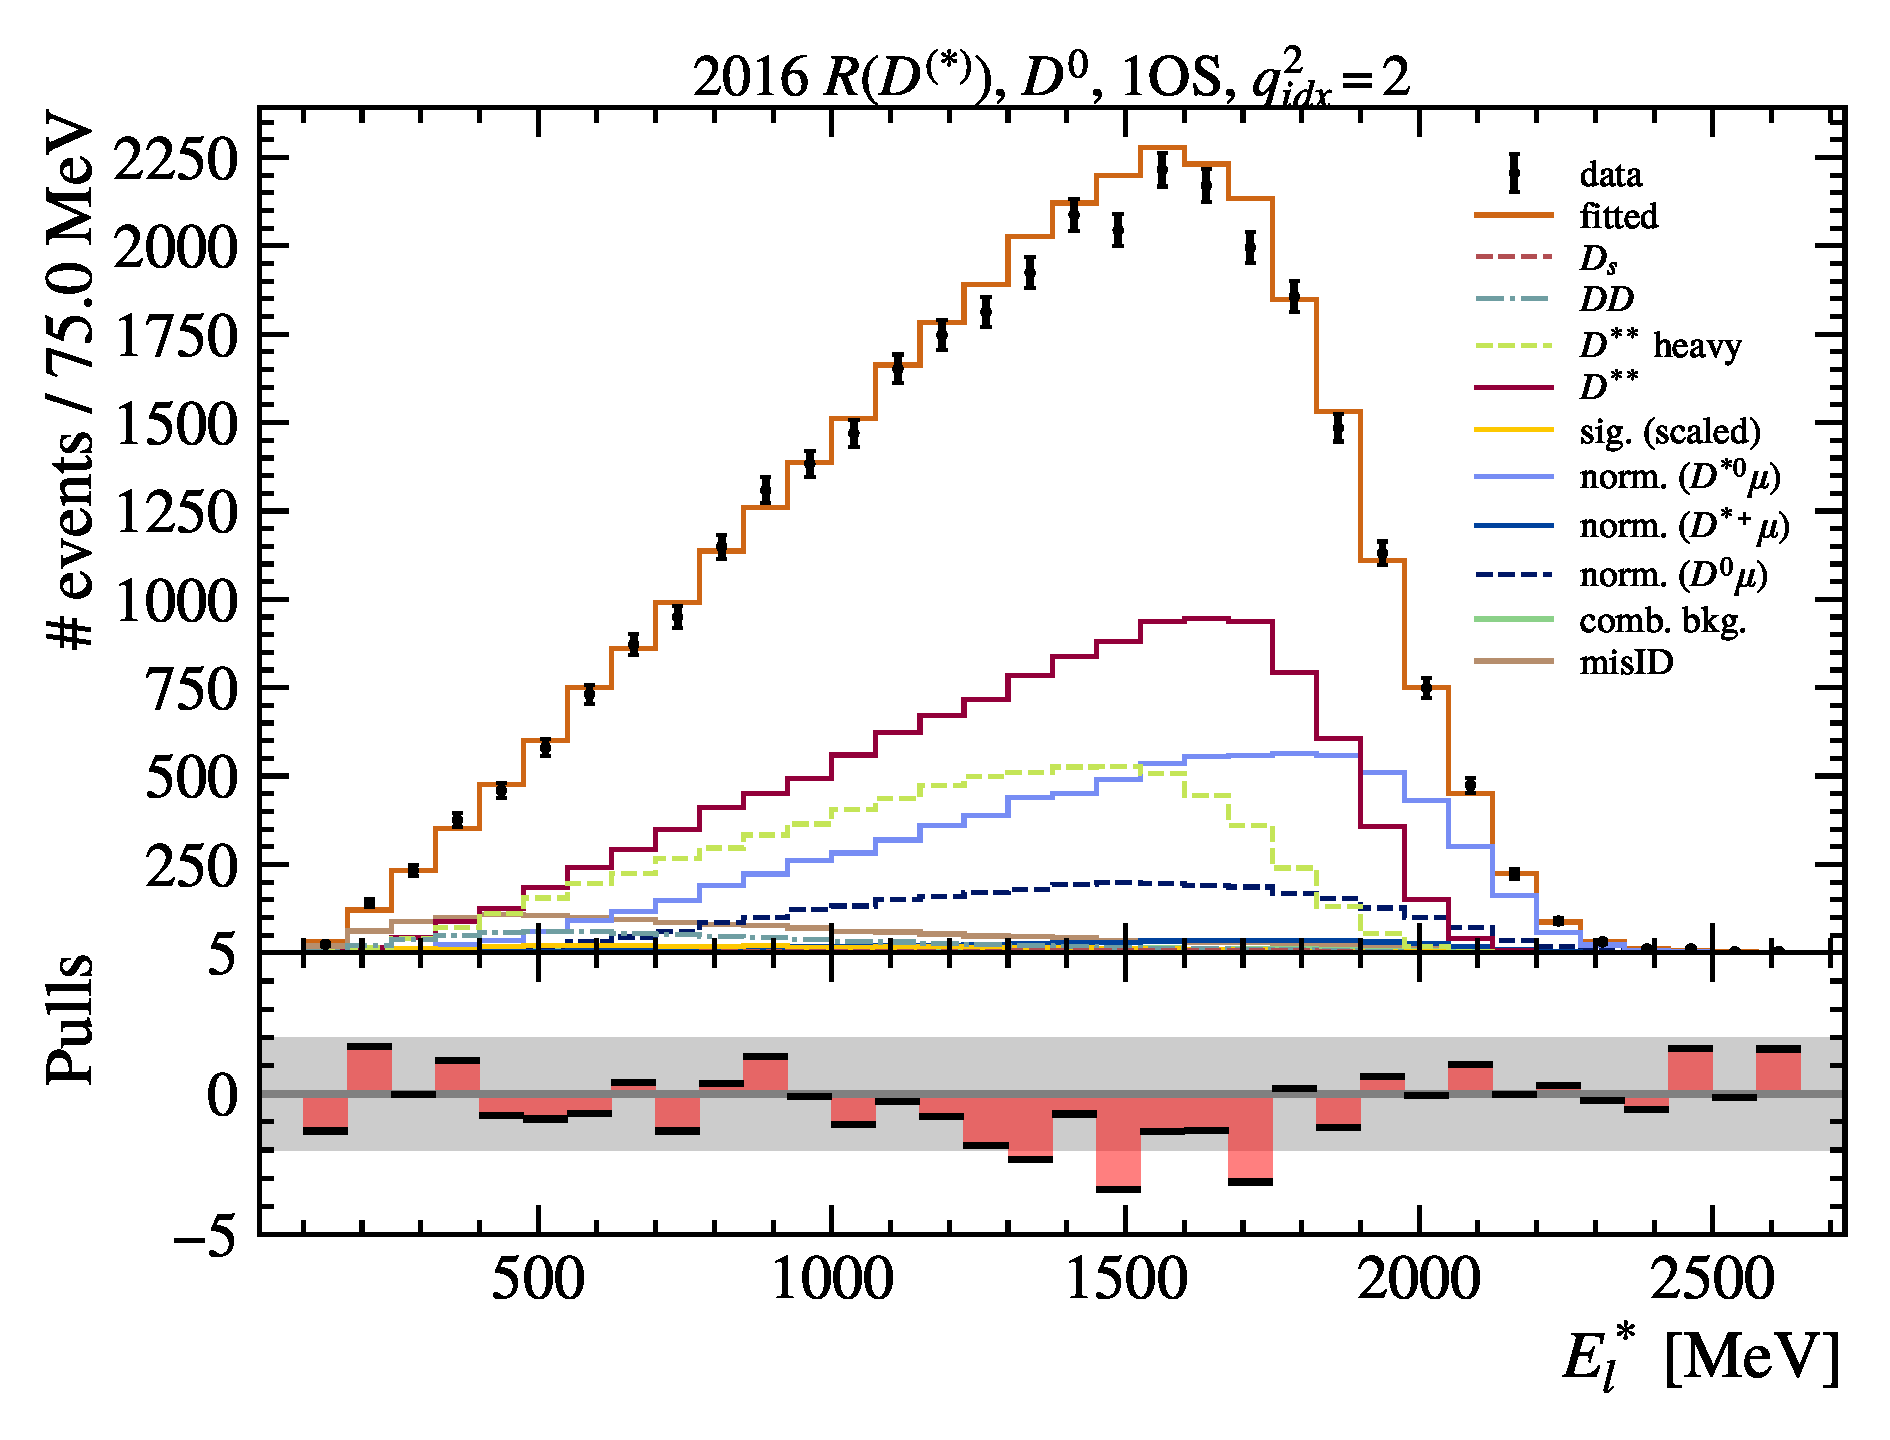
\includegraphics[width=0.24\textwidth]{./figs-fit-to-data/ctrl-fit/lines_q2_slices/fit_result-lines_q2_idx2-D0-1os-el.pdf}
    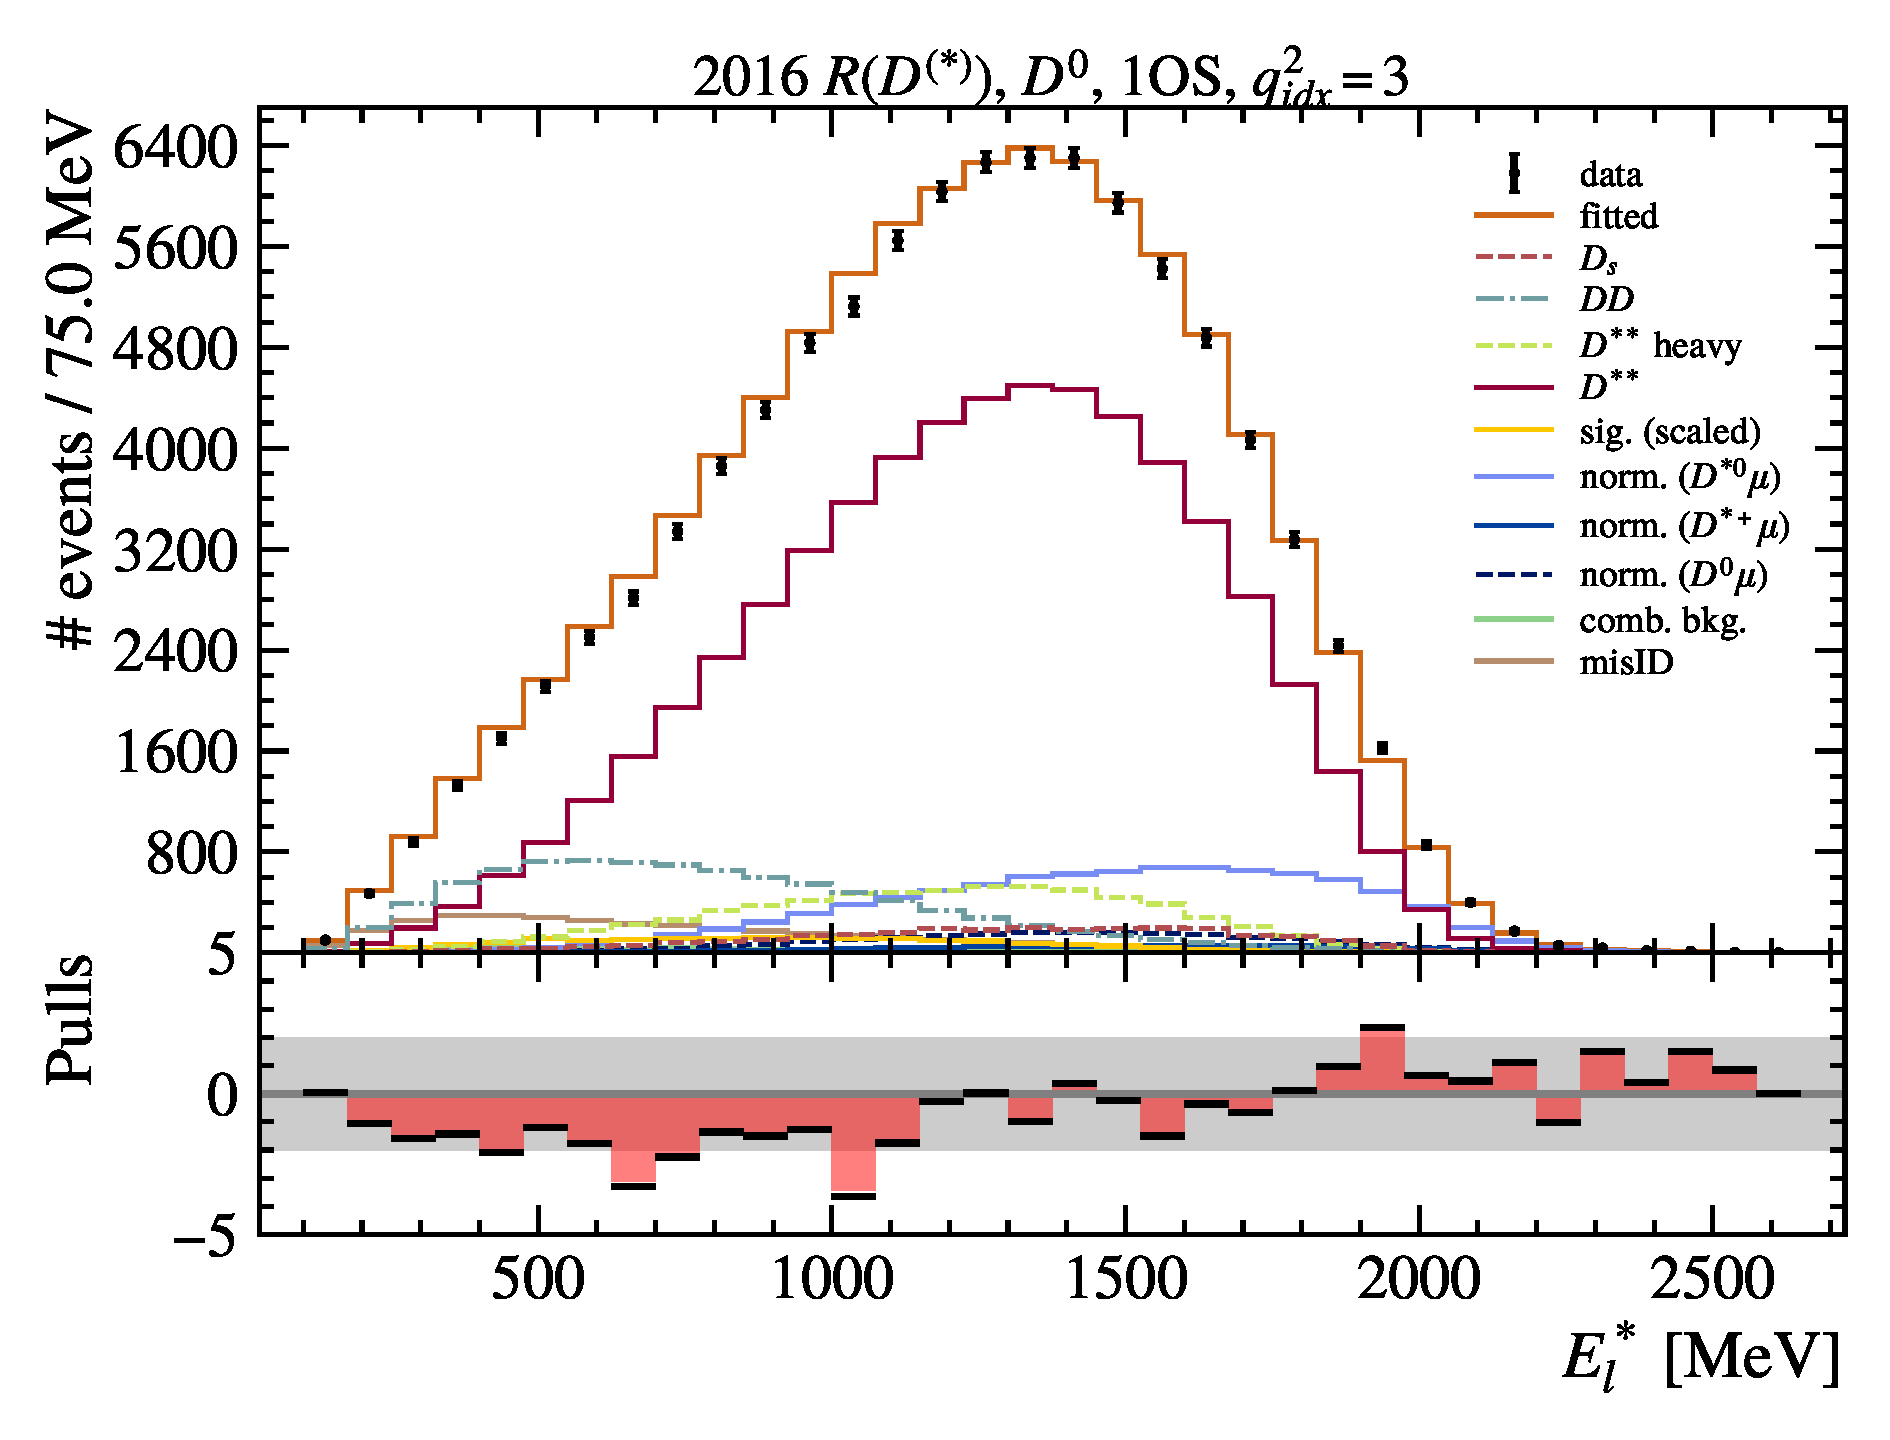
\includegraphics[width=0.24\textwidth]{./figs-fit-to-data/ctrl-fit/lines_q2_slices/fit_result-lines_q2_idx3-D0-1os-el.pdf}
    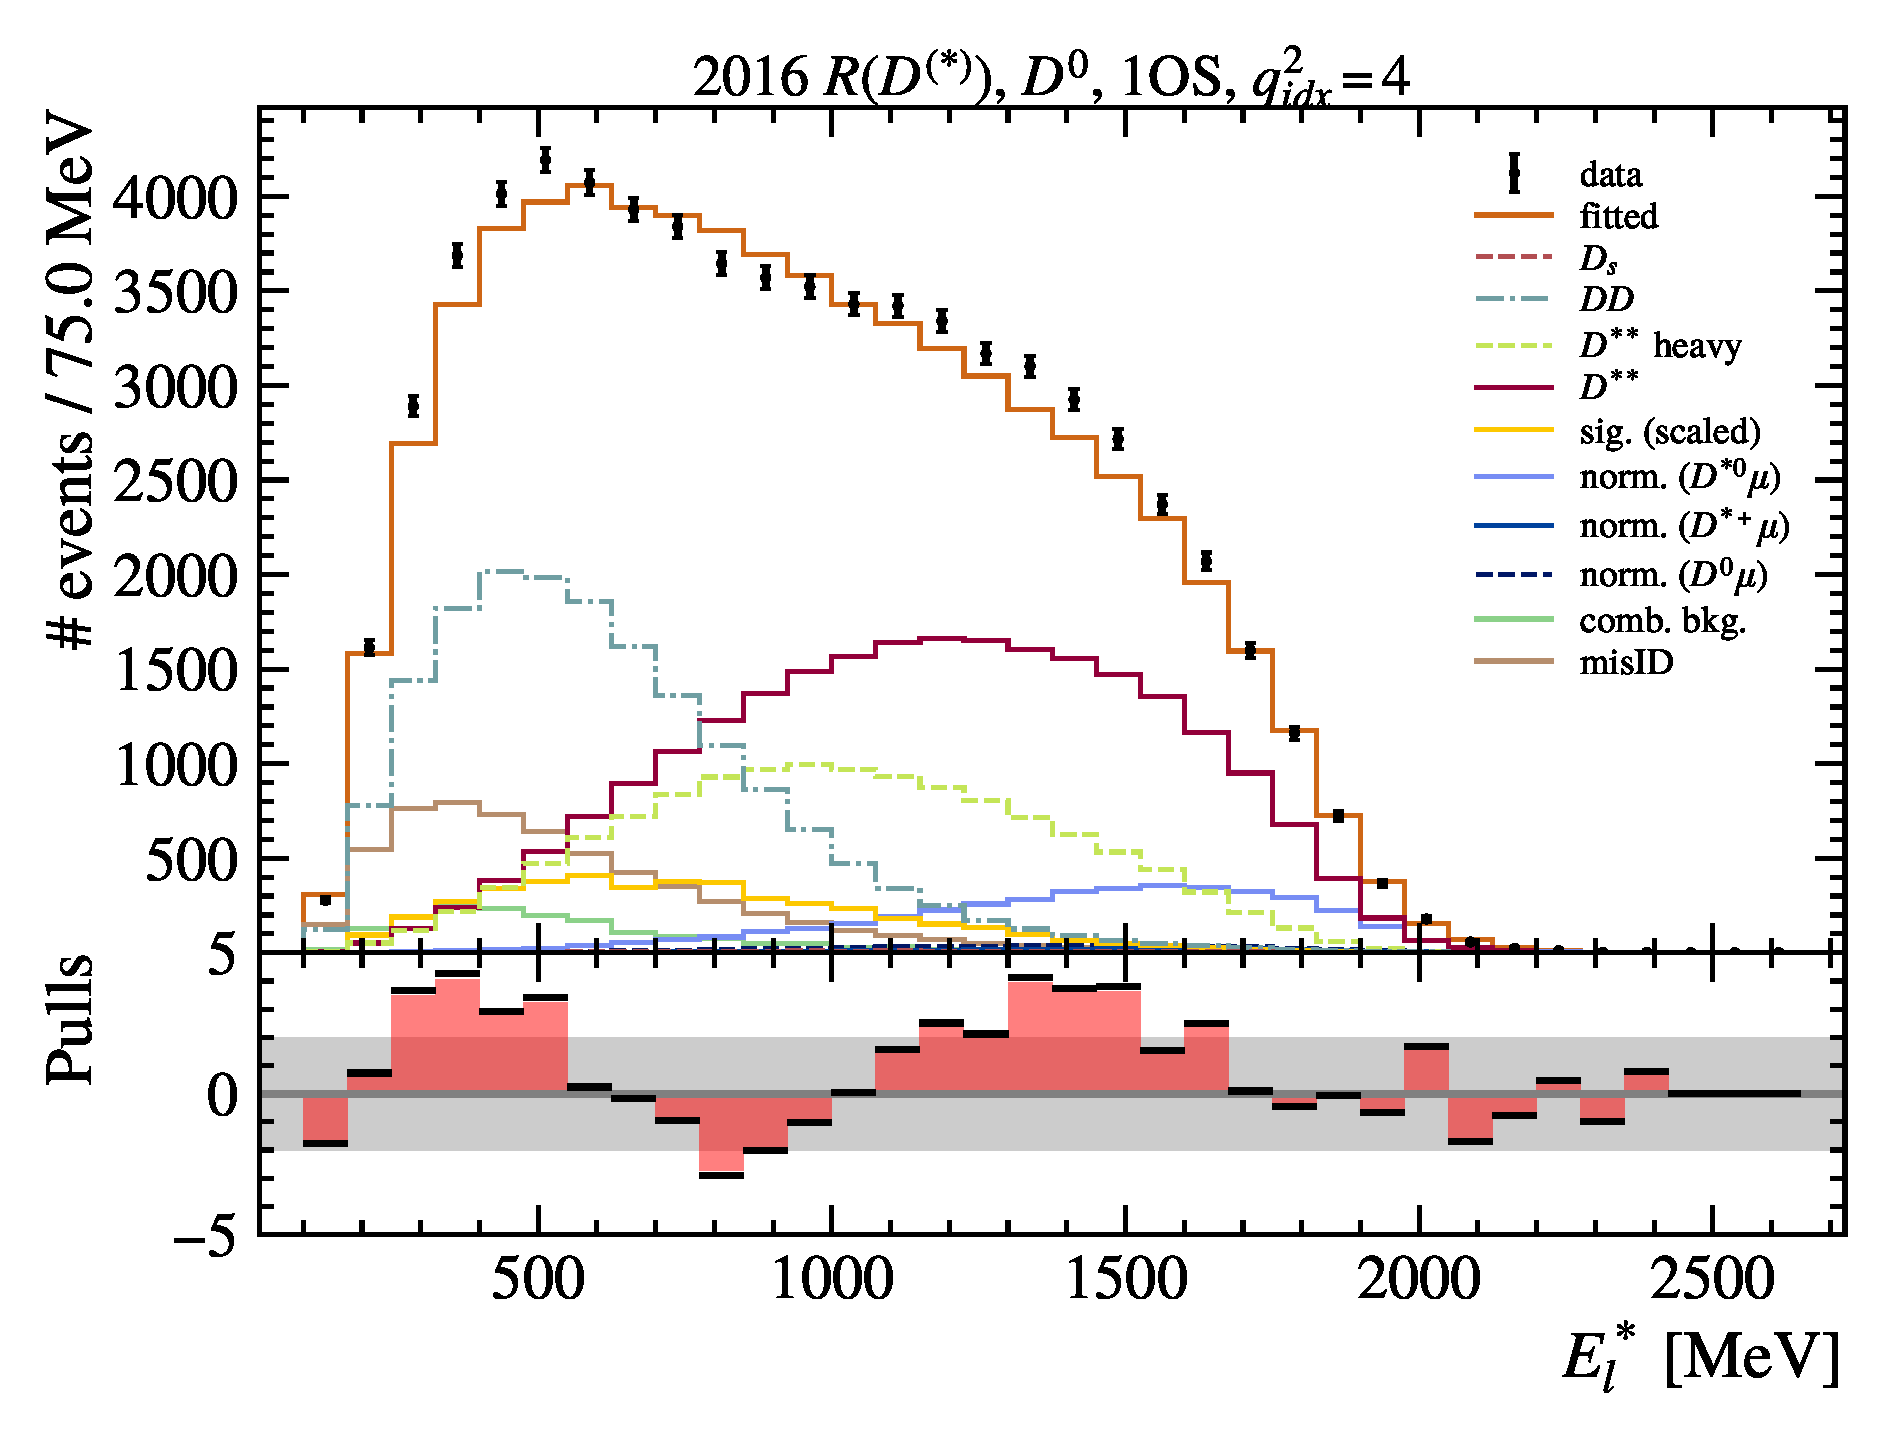
\includegraphics[width=0.24\textwidth]{./figs-fit-to-data/ctrl-fit/lines_q2_slices/fit_result-lines_q2_idx4-D0-1os-el.pdf}

    \caption{Control fit for 1OS sample, \Dz channel.}
    \label{fig:ctrl-1os-d0}
\end{figure}

\begin{figure}[htb]
    \centering
    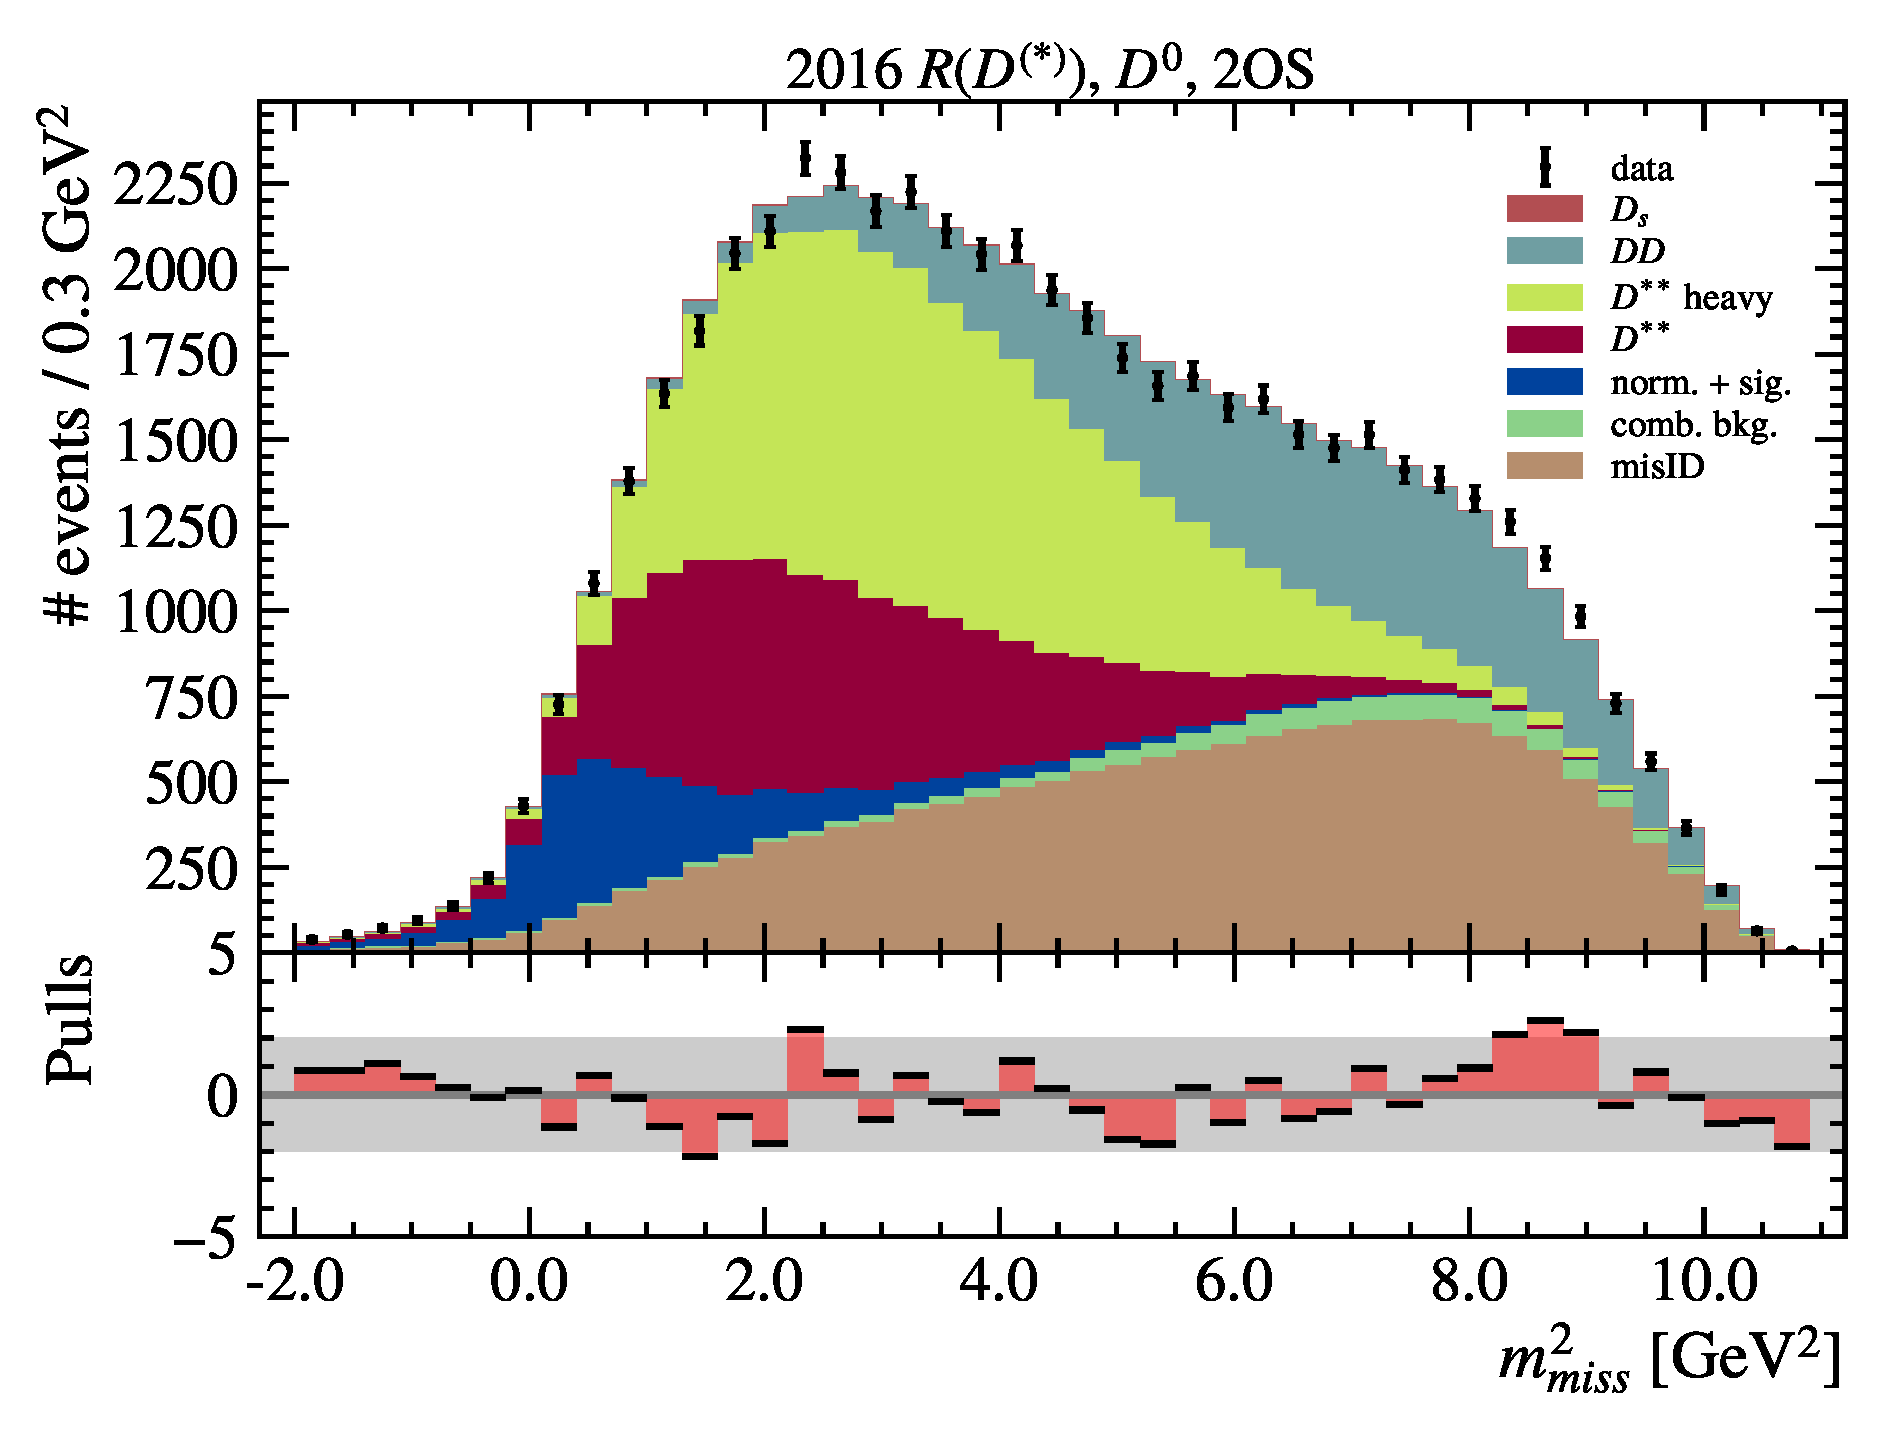
\includegraphics[width=0.32\textwidth]{./figs-fit-to-data/ctrl-fit/stacked/fit_result-stacked-D0-2os-mmiss2.pdf}
    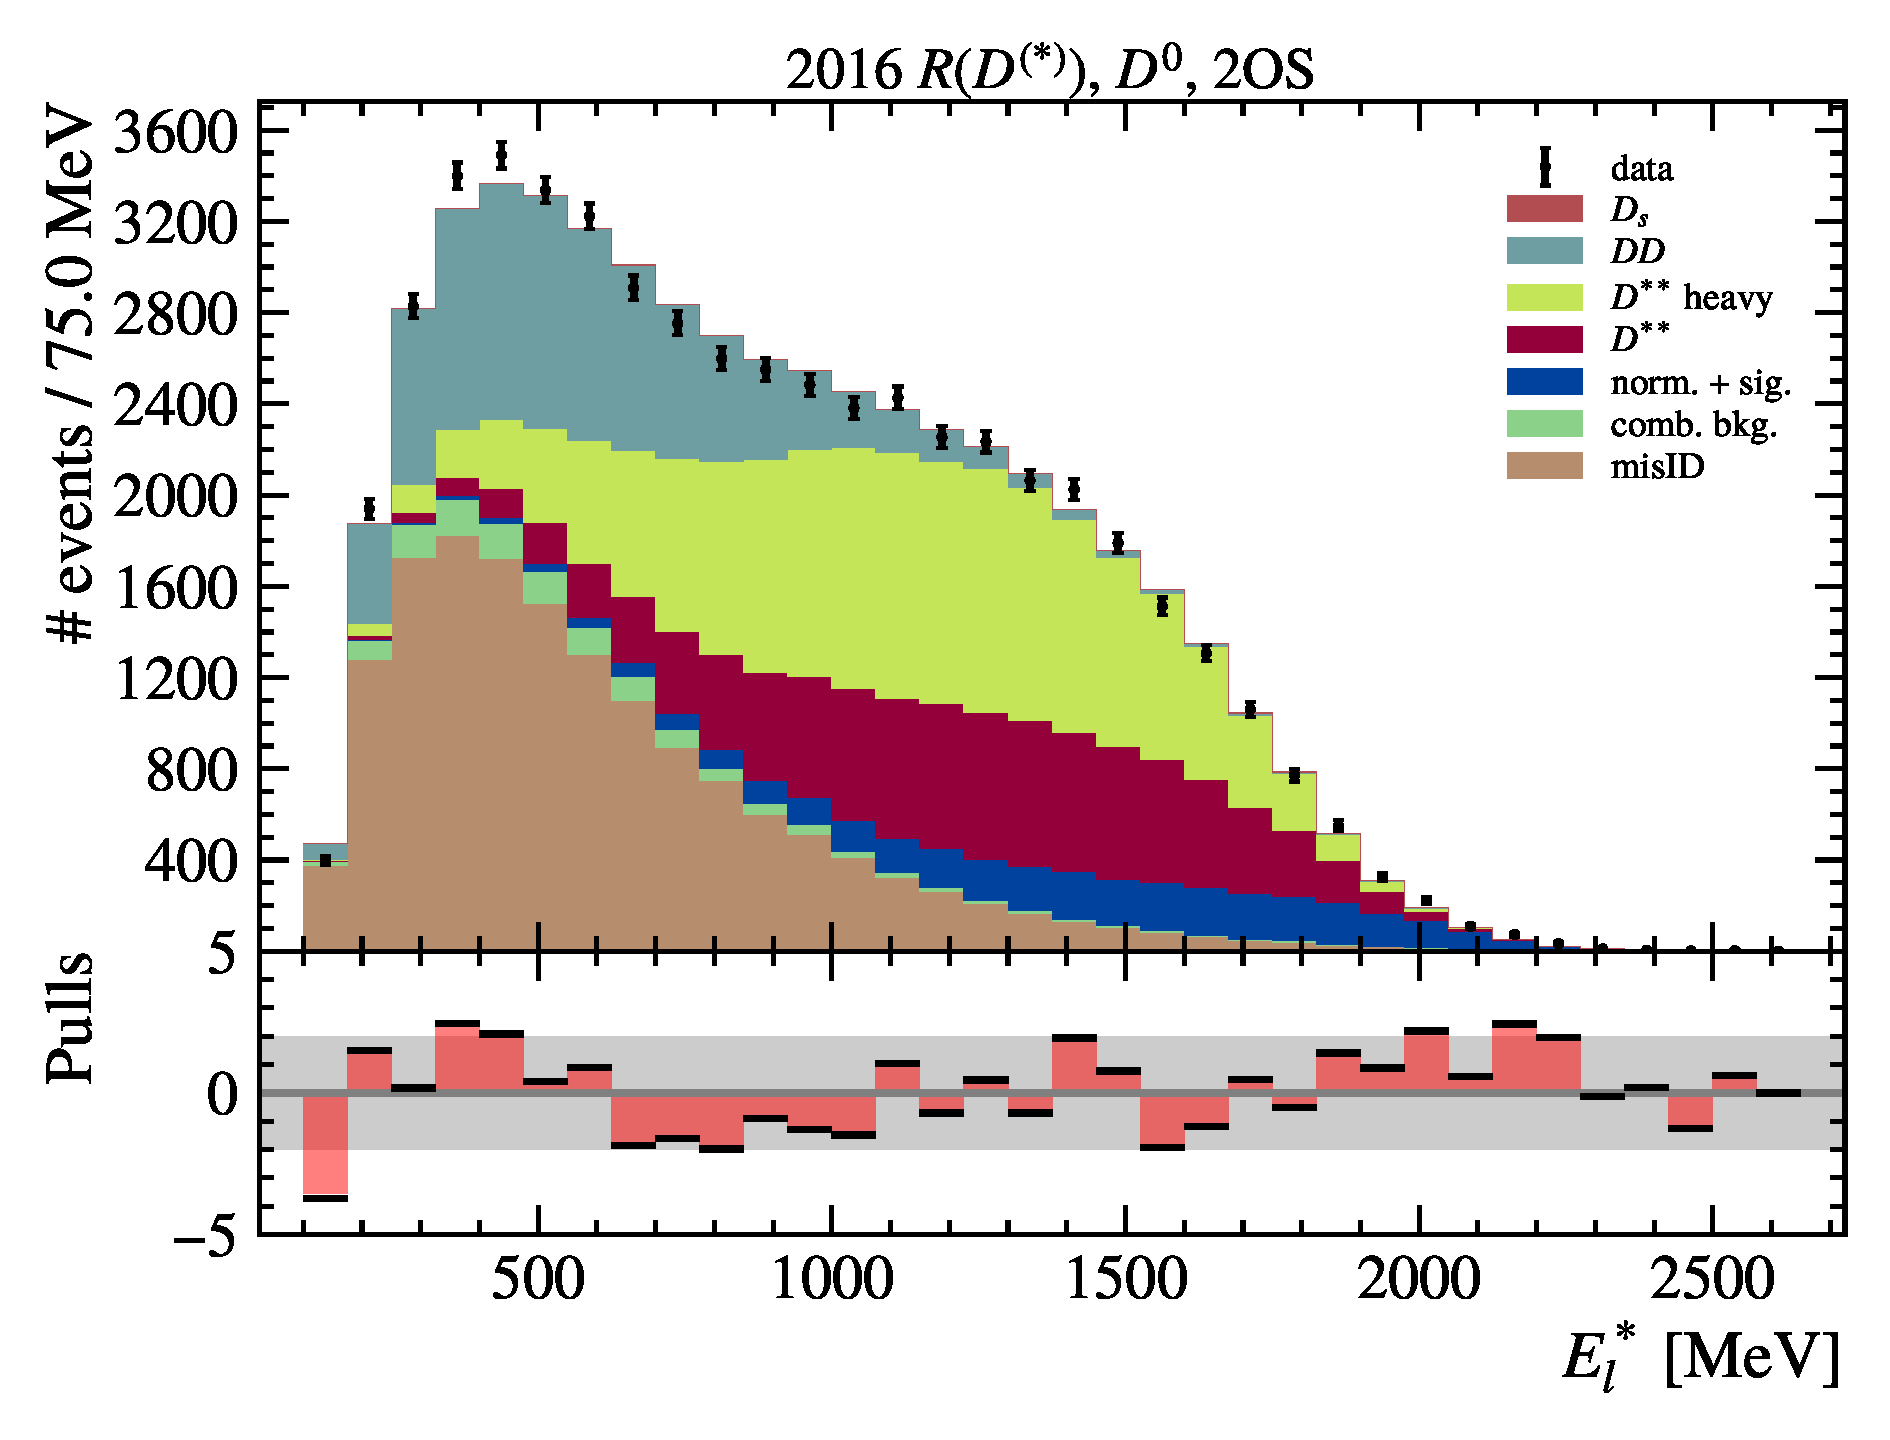
\includegraphics[width=0.32\textwidth]{./figs-fit-to-data/ctrl-fit/stacked/fit_result-stacked-D0-2os-el.pdf}
    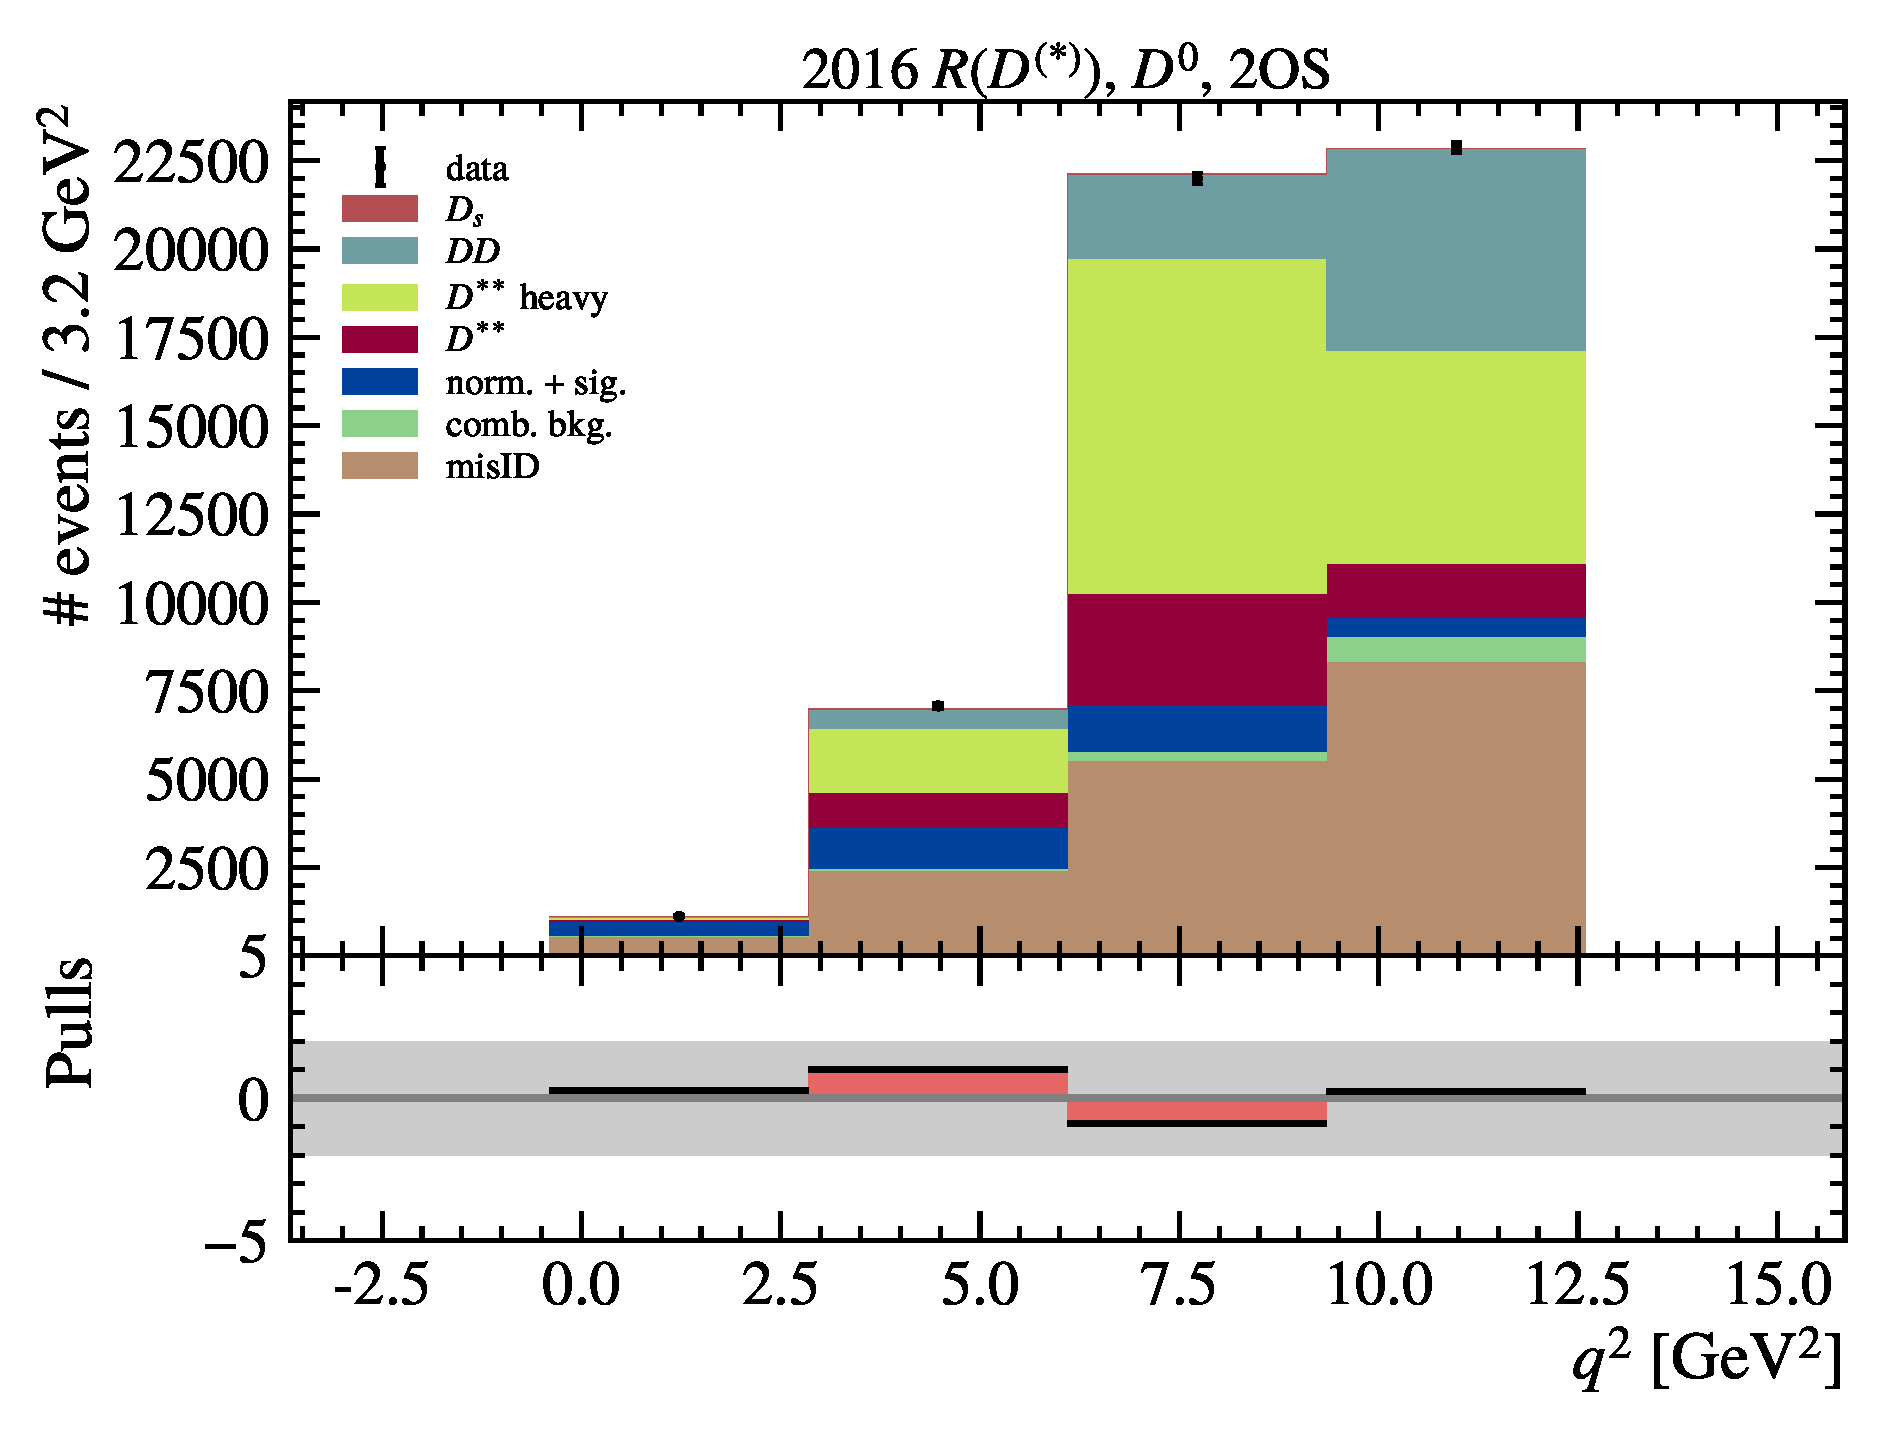
\includegraphics[width=0.32\textwidth]{./figs-fit-to-data/ctrl-fit/stacked/fit_result-stacked-D0-2os-q2.pdf}

    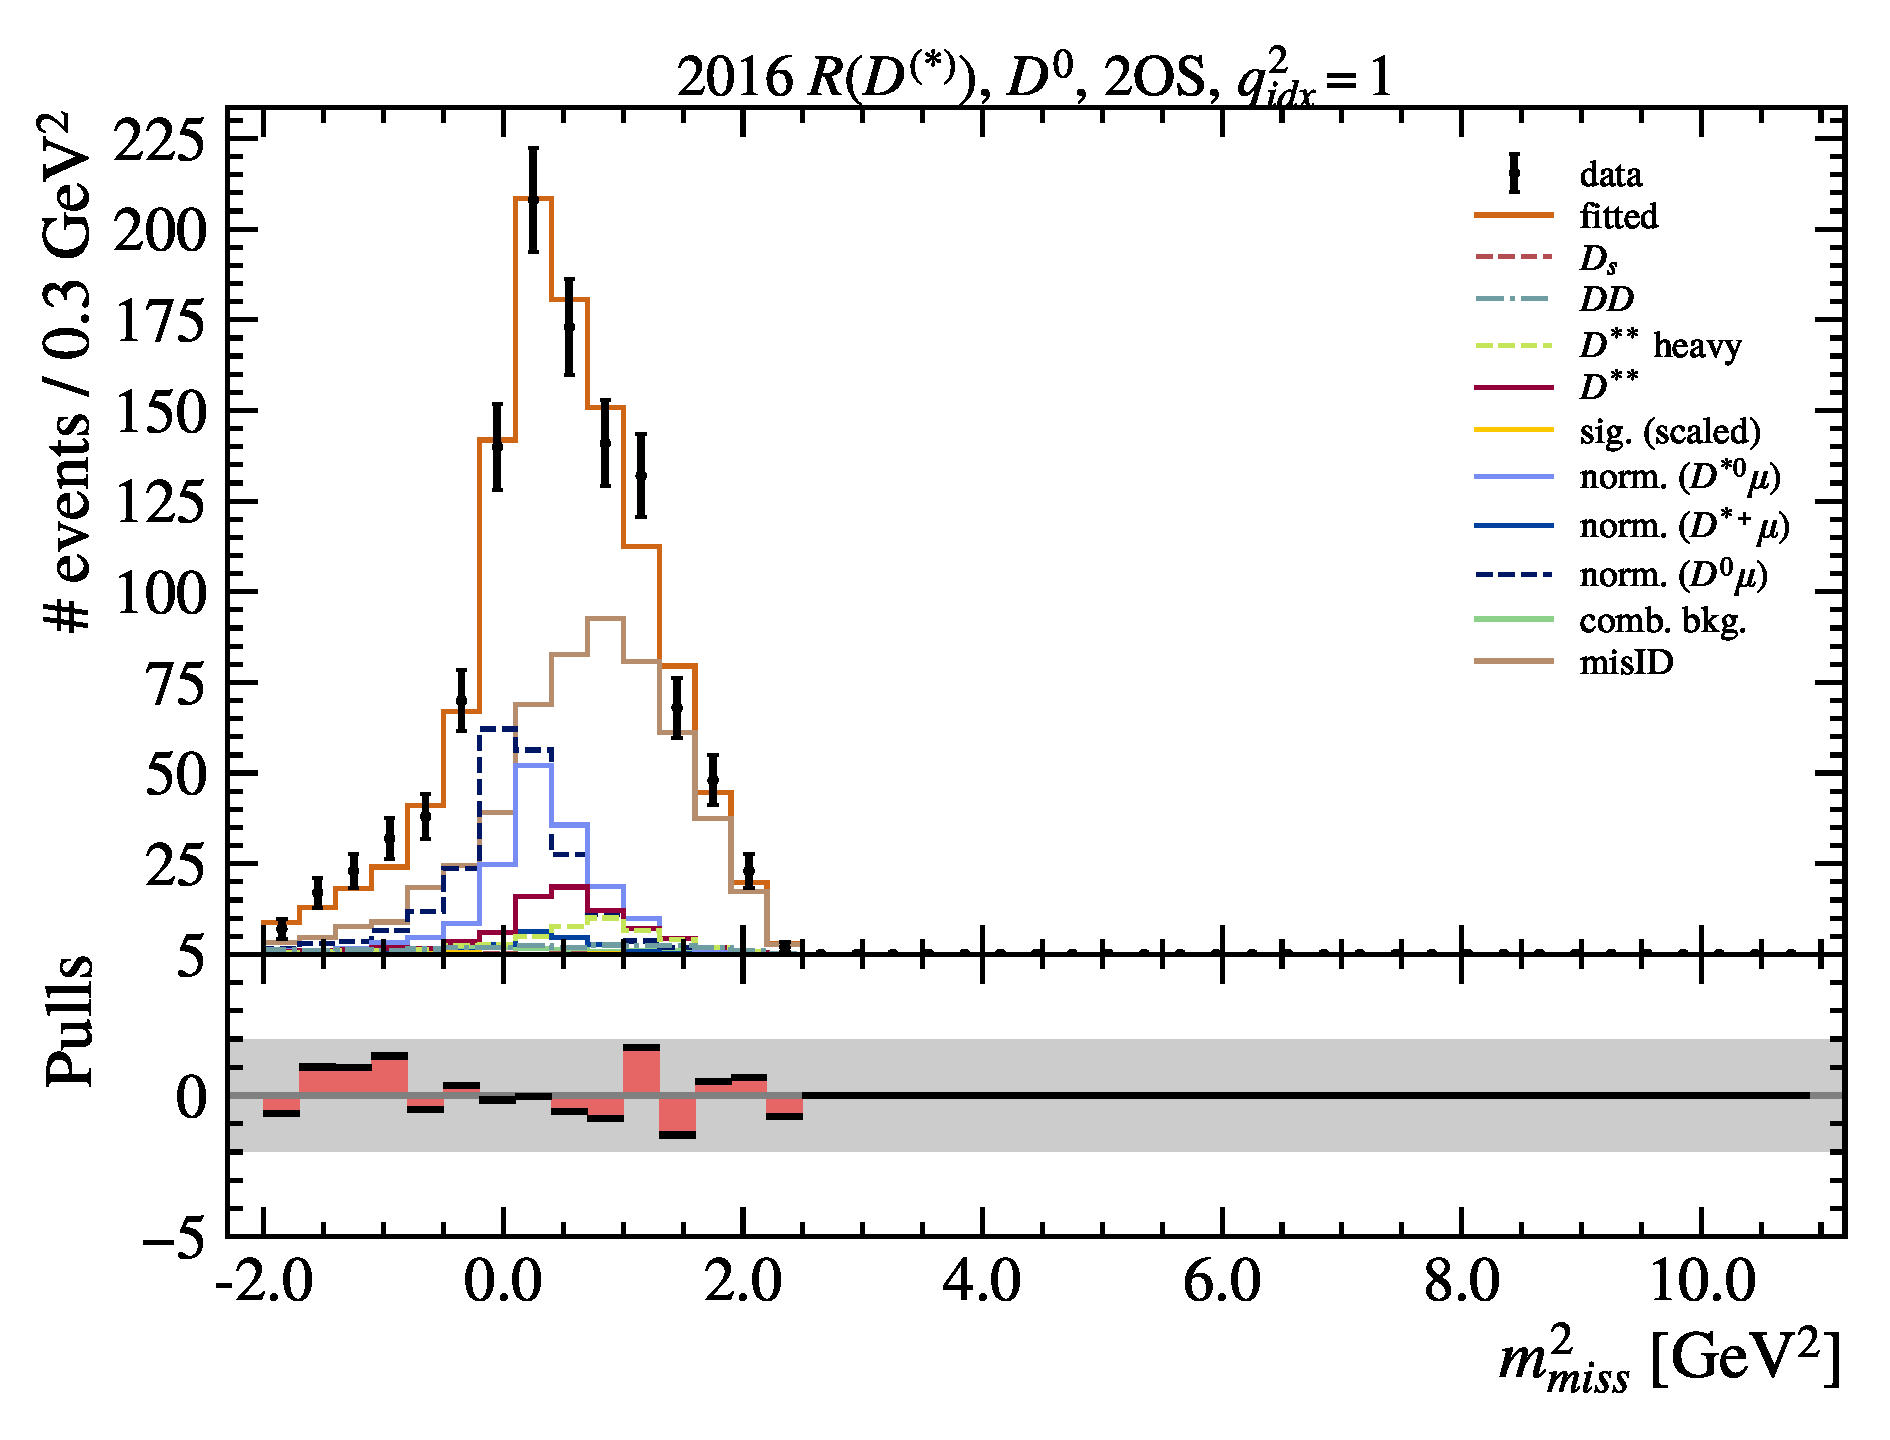
\includegraphics[width=0.24\textwidth]{./figs-fit-to-data/ctrl-fit/lines_q2_slices/fit_result-lines_q2_idx1-D0-2os-mmiss2.pdf}
    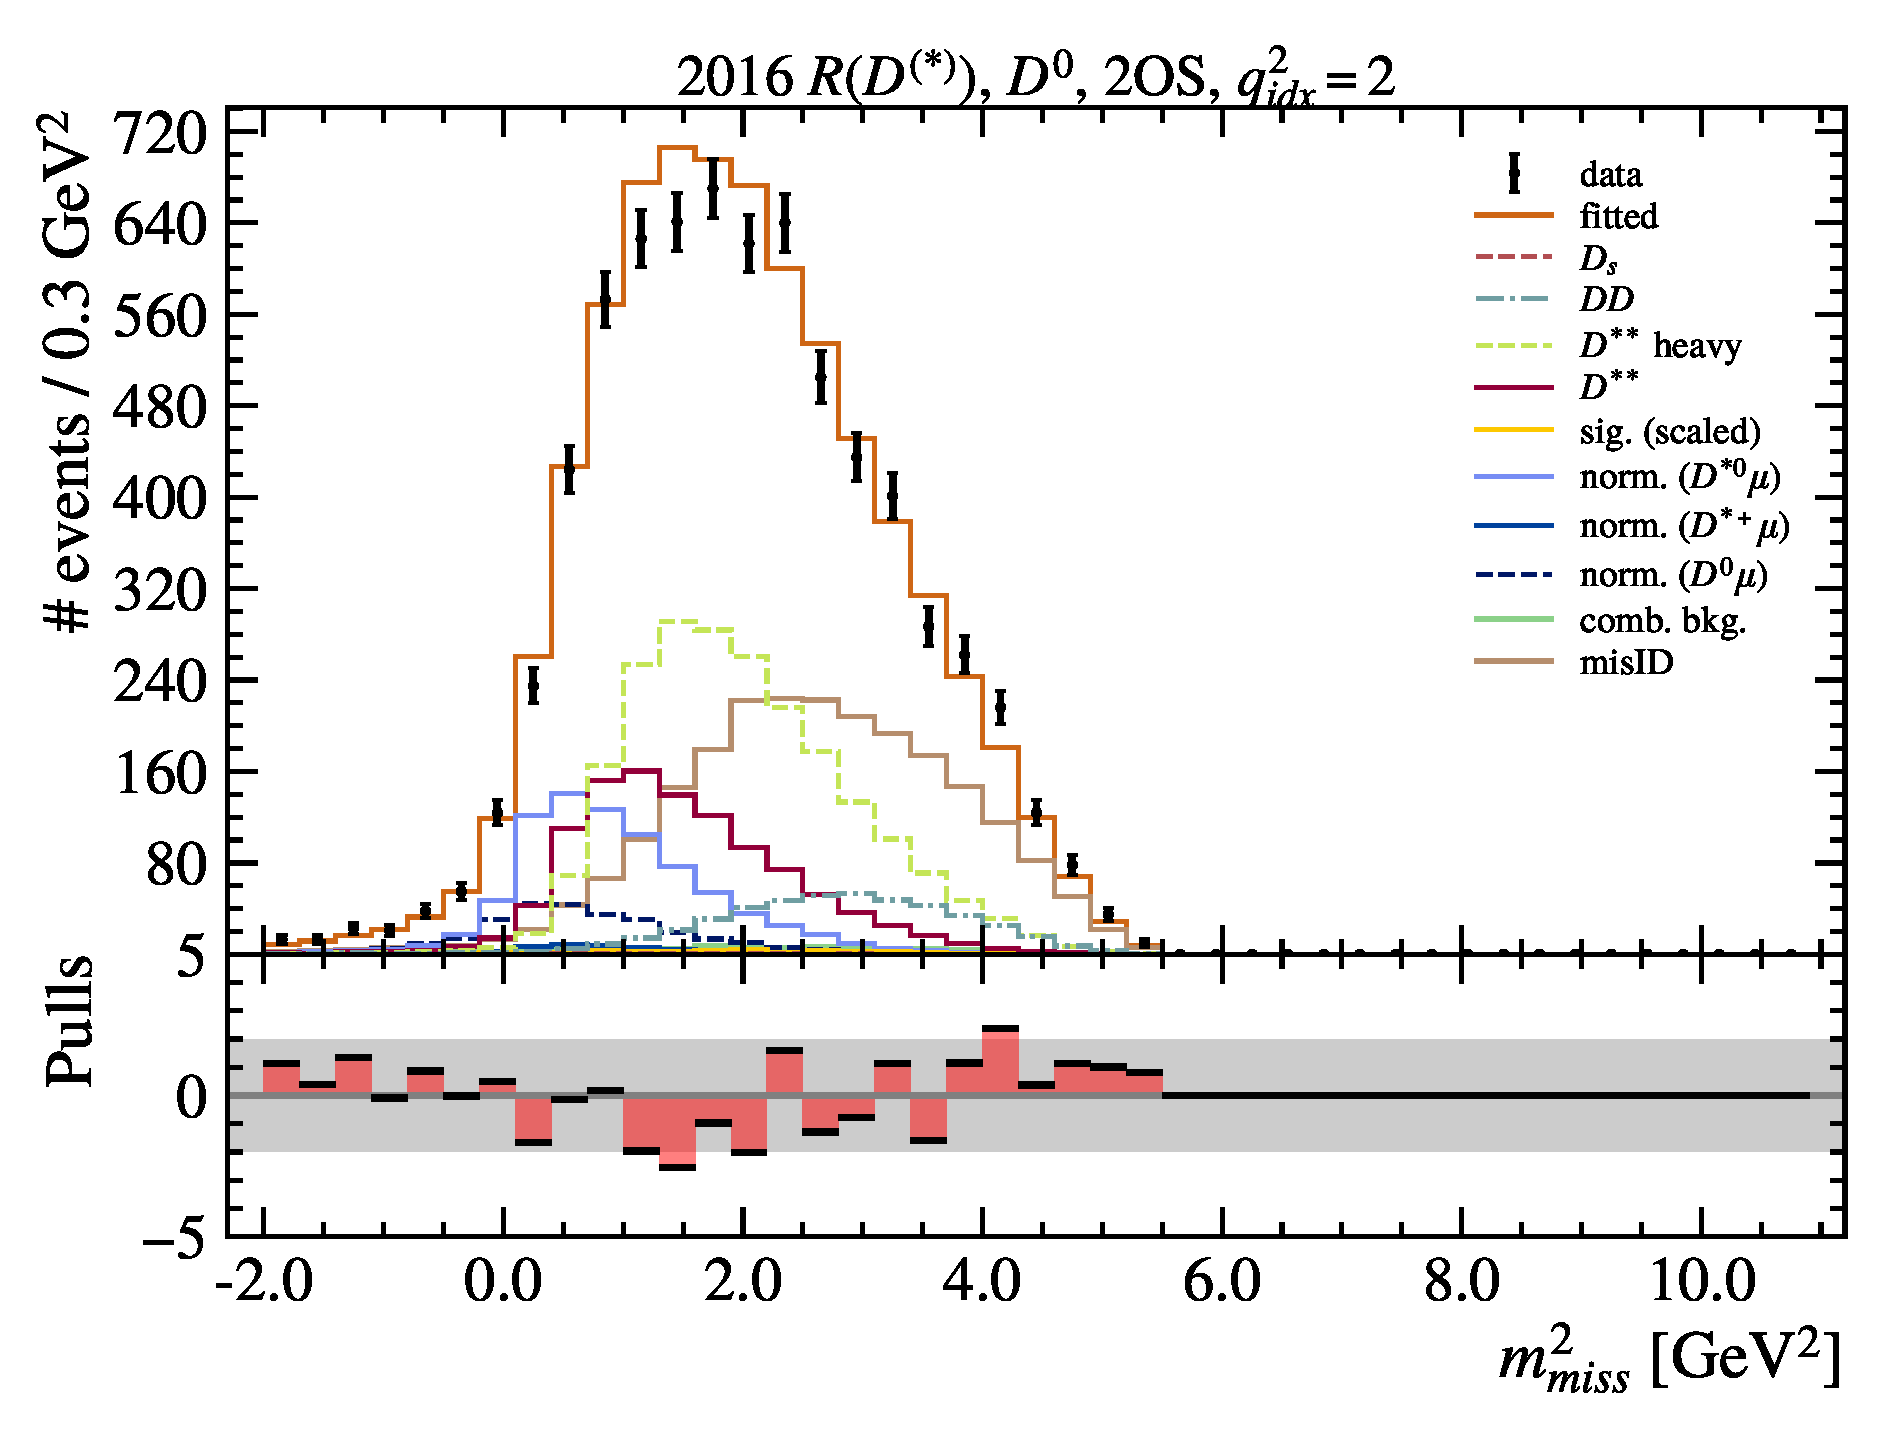
\includegraphics[width=0.24\textwidth]{./figs-fit-to-data/ctrl-fit/lines_q2_slices/fit_result-lines_q2_idx2-D0-2os-mmiss2.pdf}
    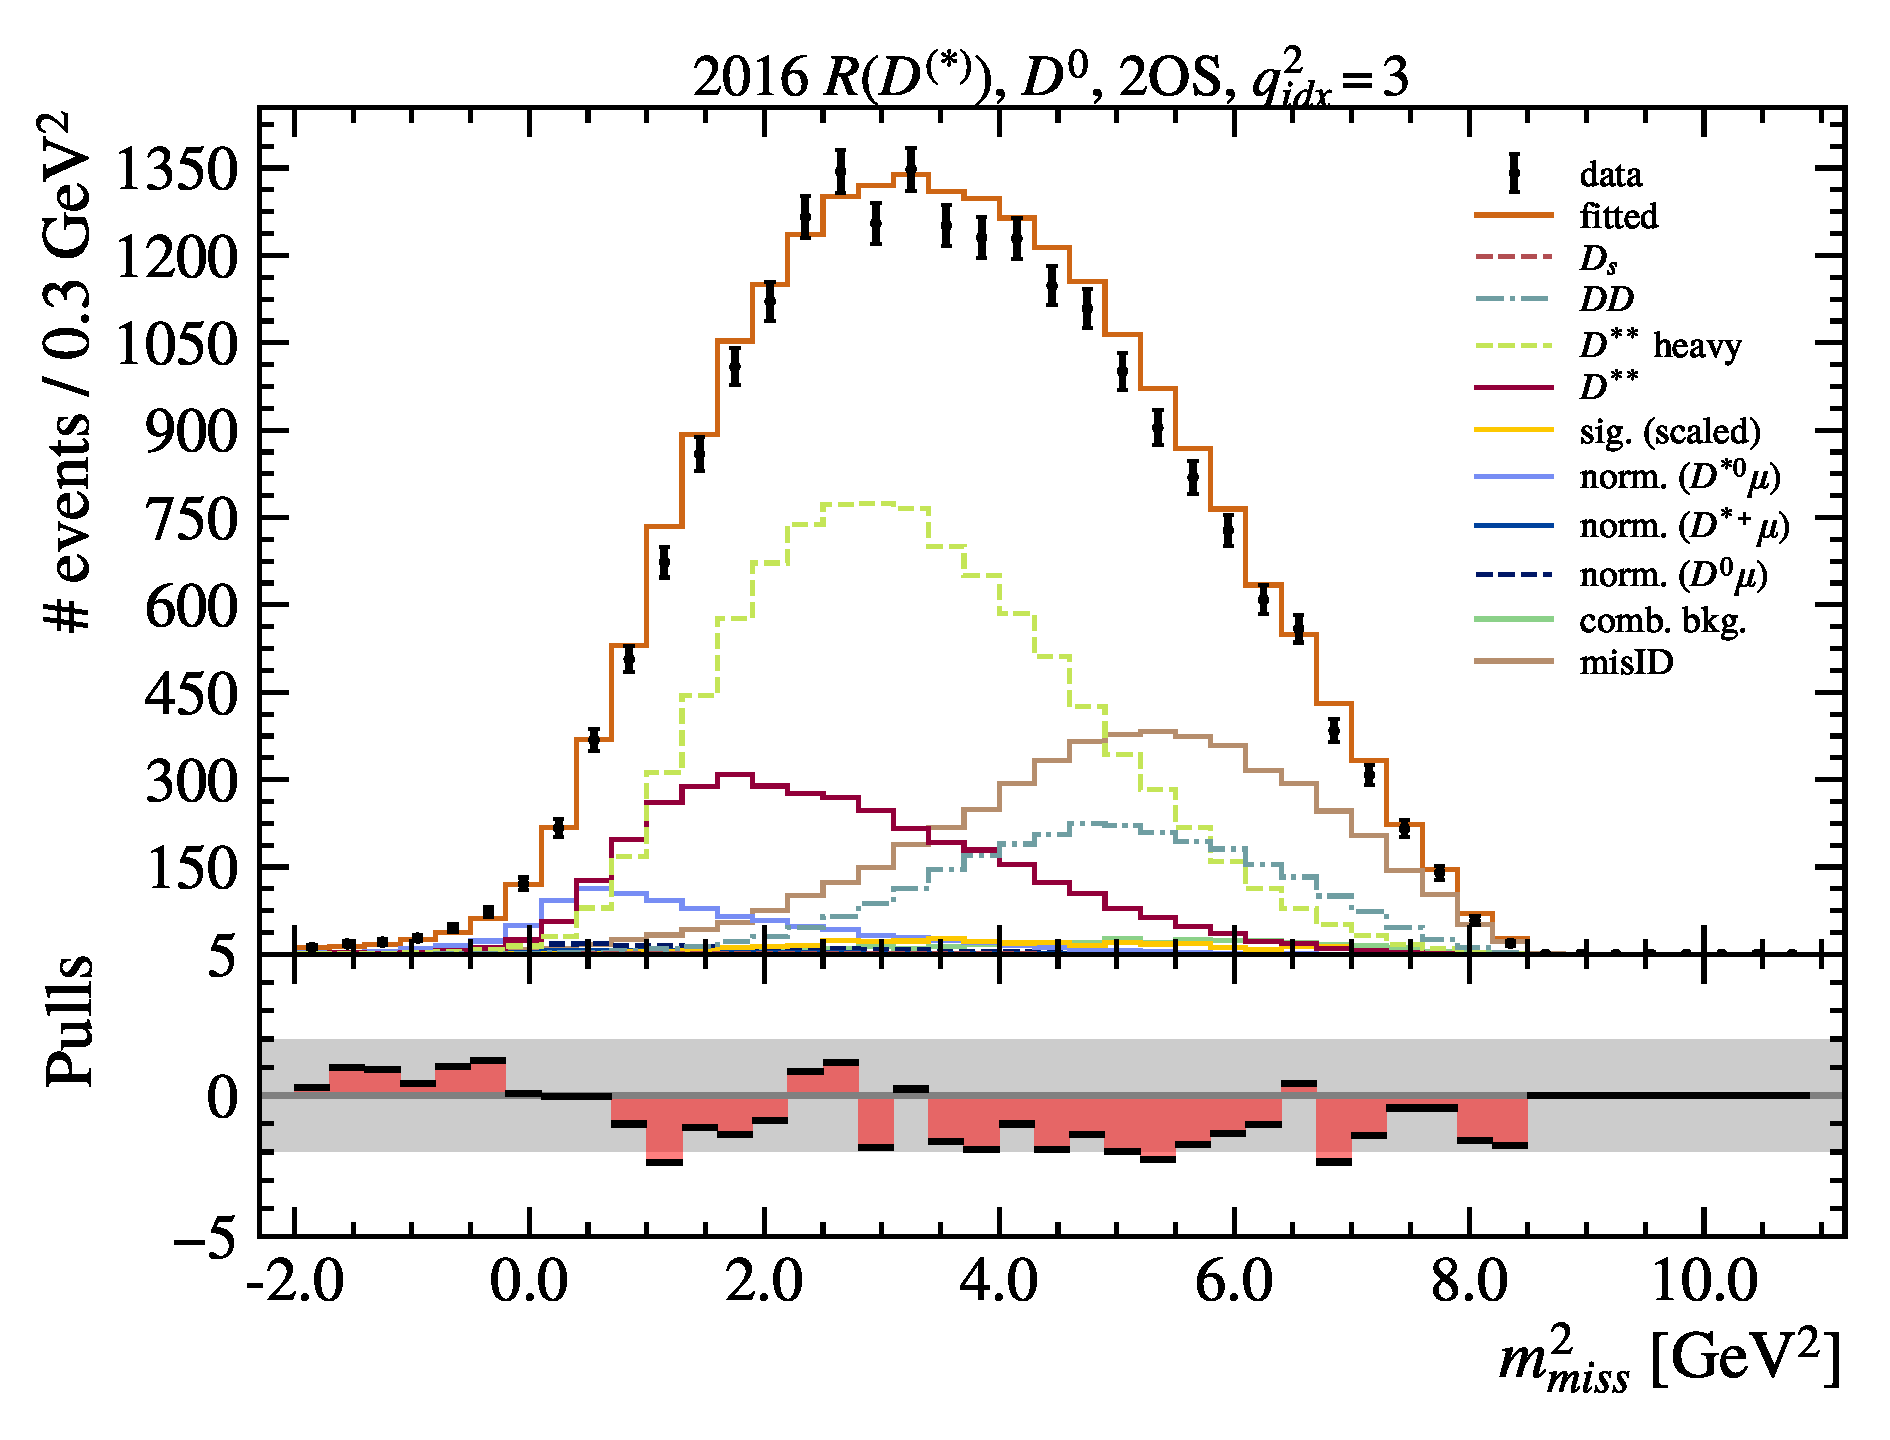
\includegraphics[width=0.24\textwidth]{./figs-fit-to-data/ctrl-fit/lines_q2_slices/fit_result-lines_q2_idx3-D0-2os-mmiss2.pdf}
    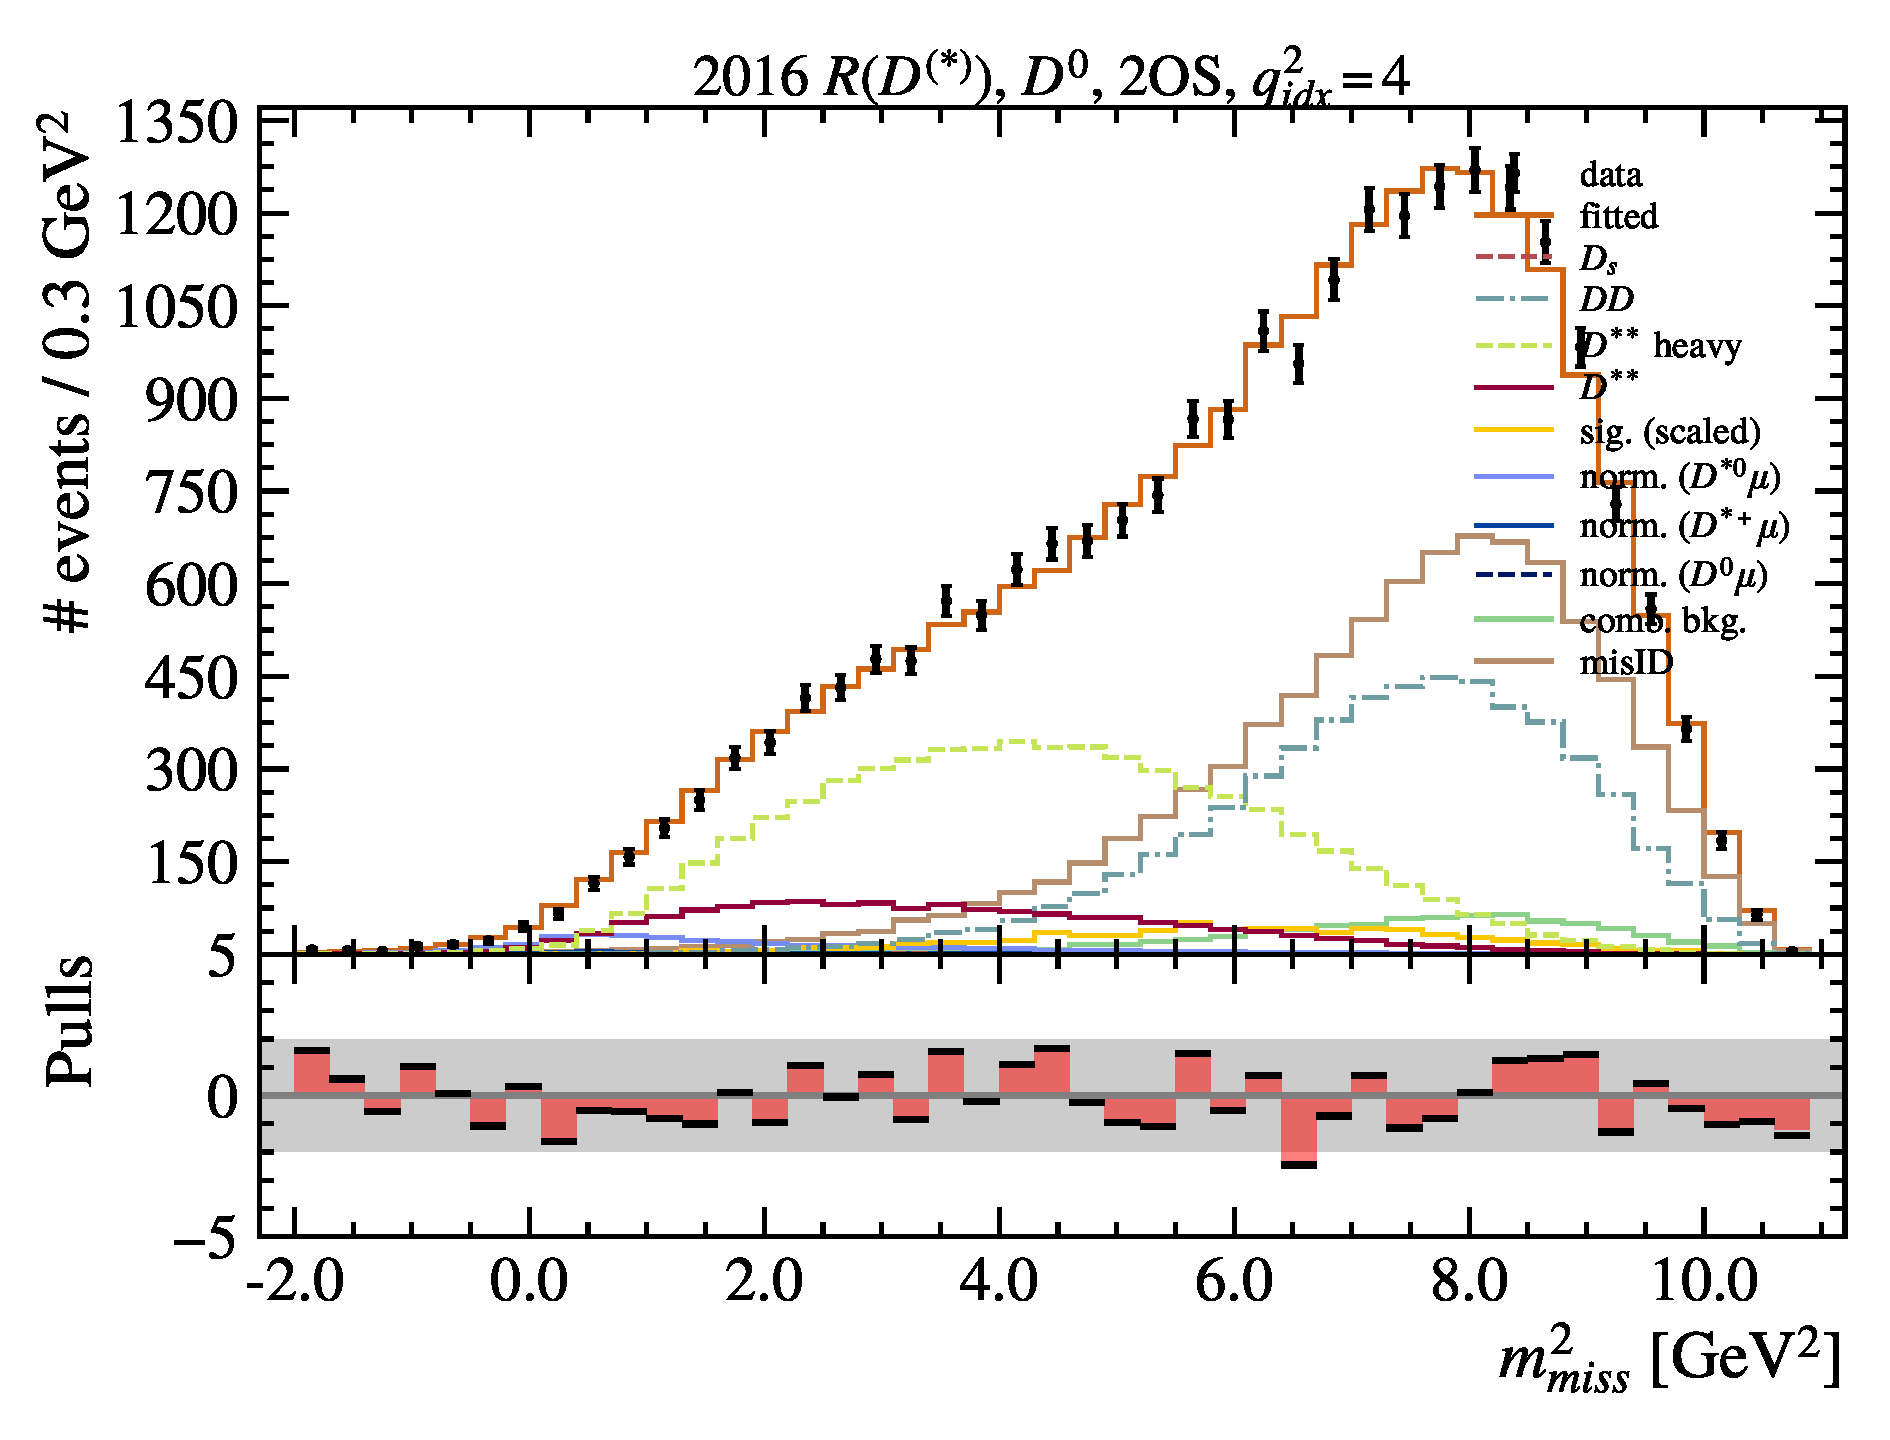
\includegraphics[width=0.24\textwidth]{./figs-fit-to-data/ctrl-fit/lines_q2_slices/fit_result-lines_q2_idx4-D0-2os-mmiss2.pdf}

    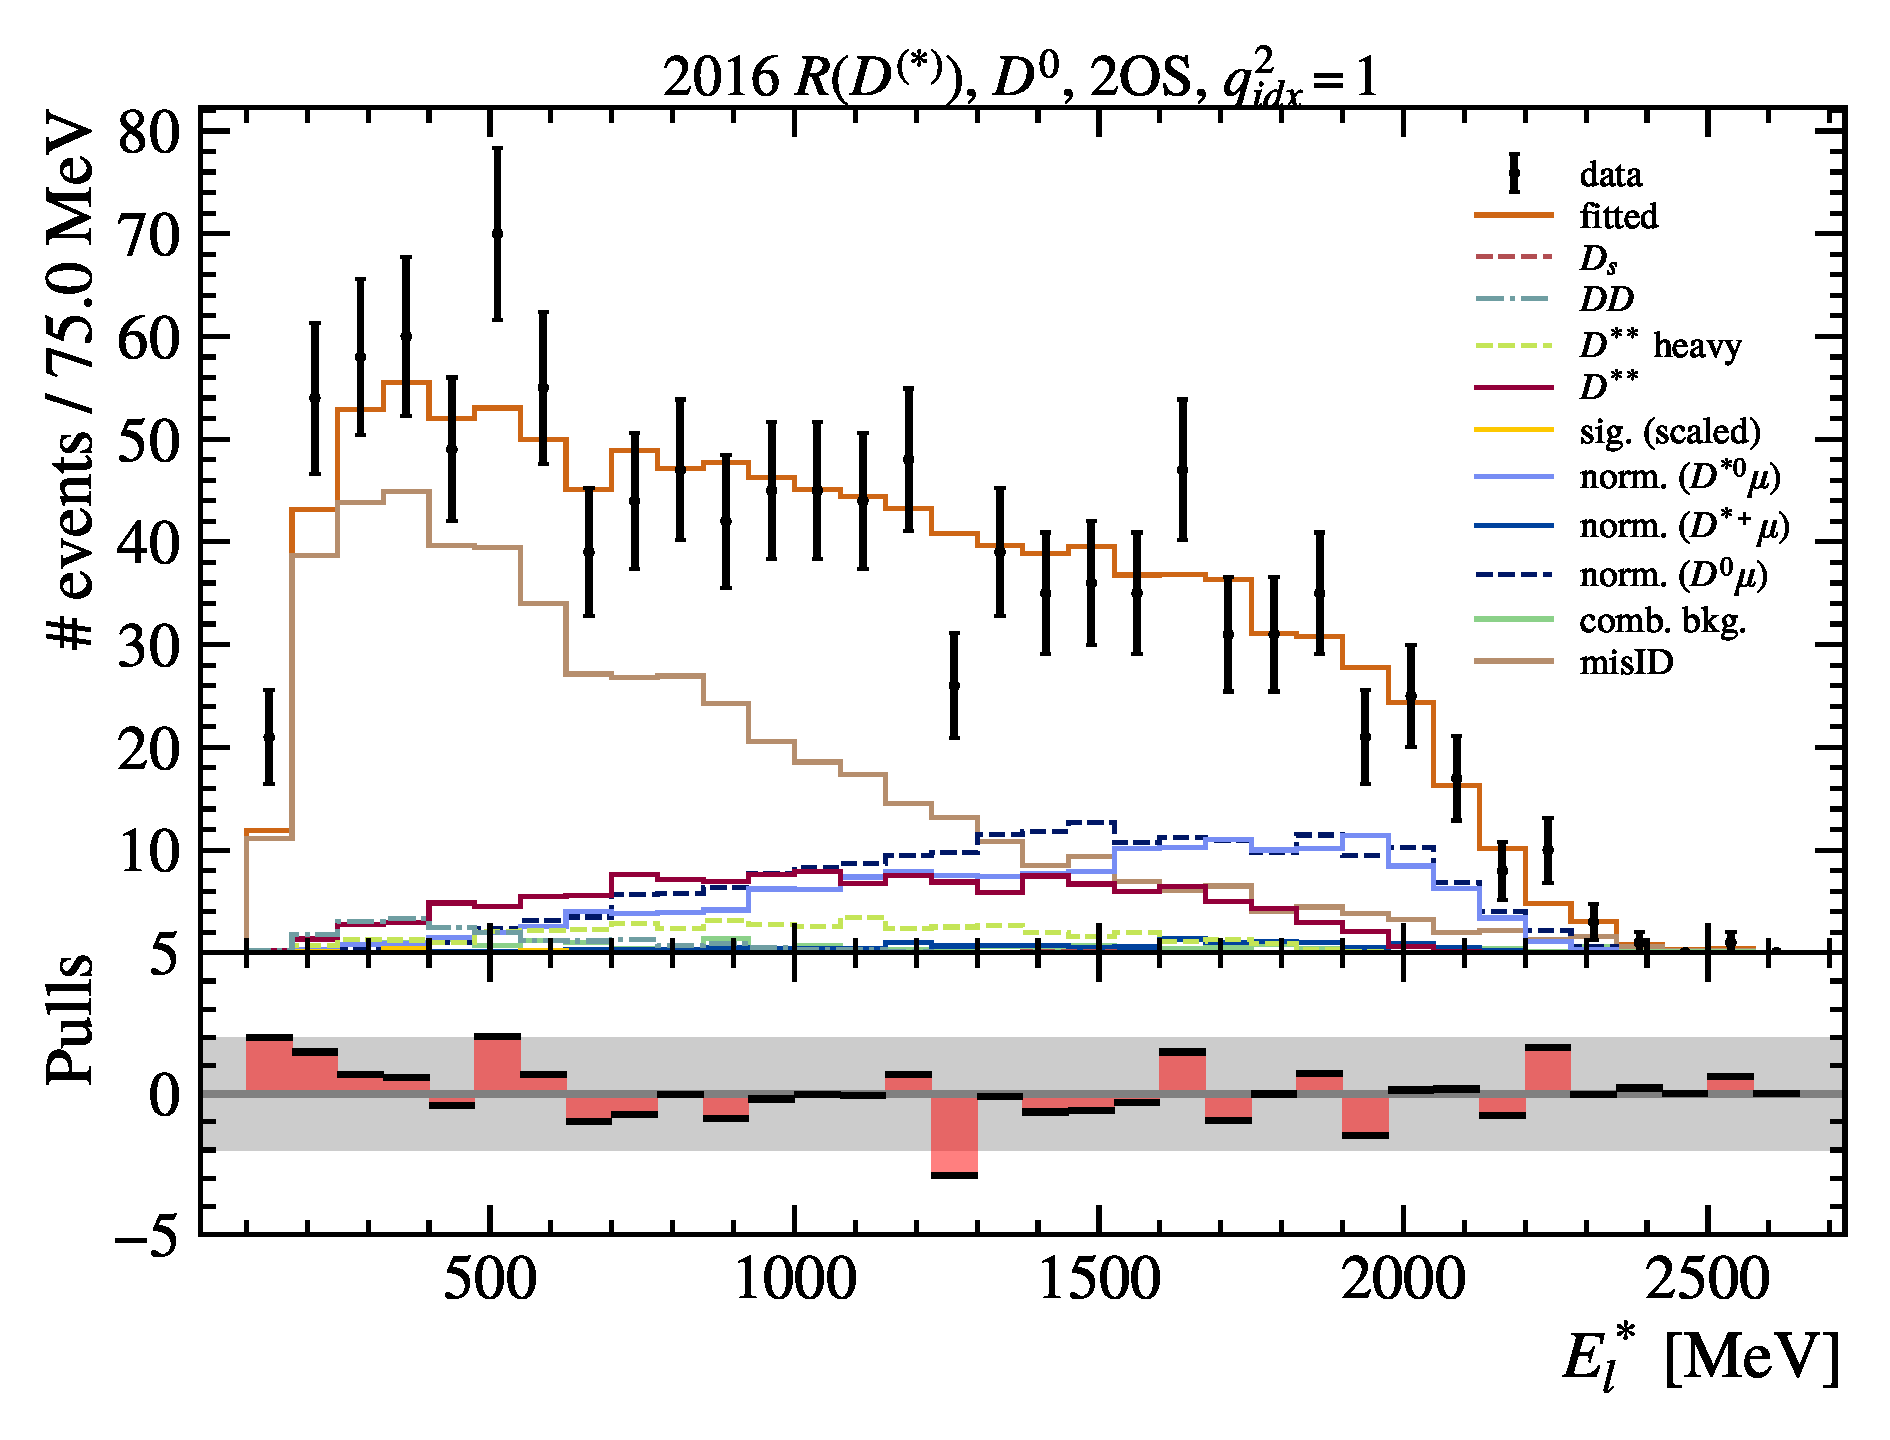
\includegraphics[width=0.24\textwidth]{./figs-fit-to-data/ctrl-fit/lines_q2_slices/fit_result-lines_q2_idx1-D0-2os-el.pdf}
    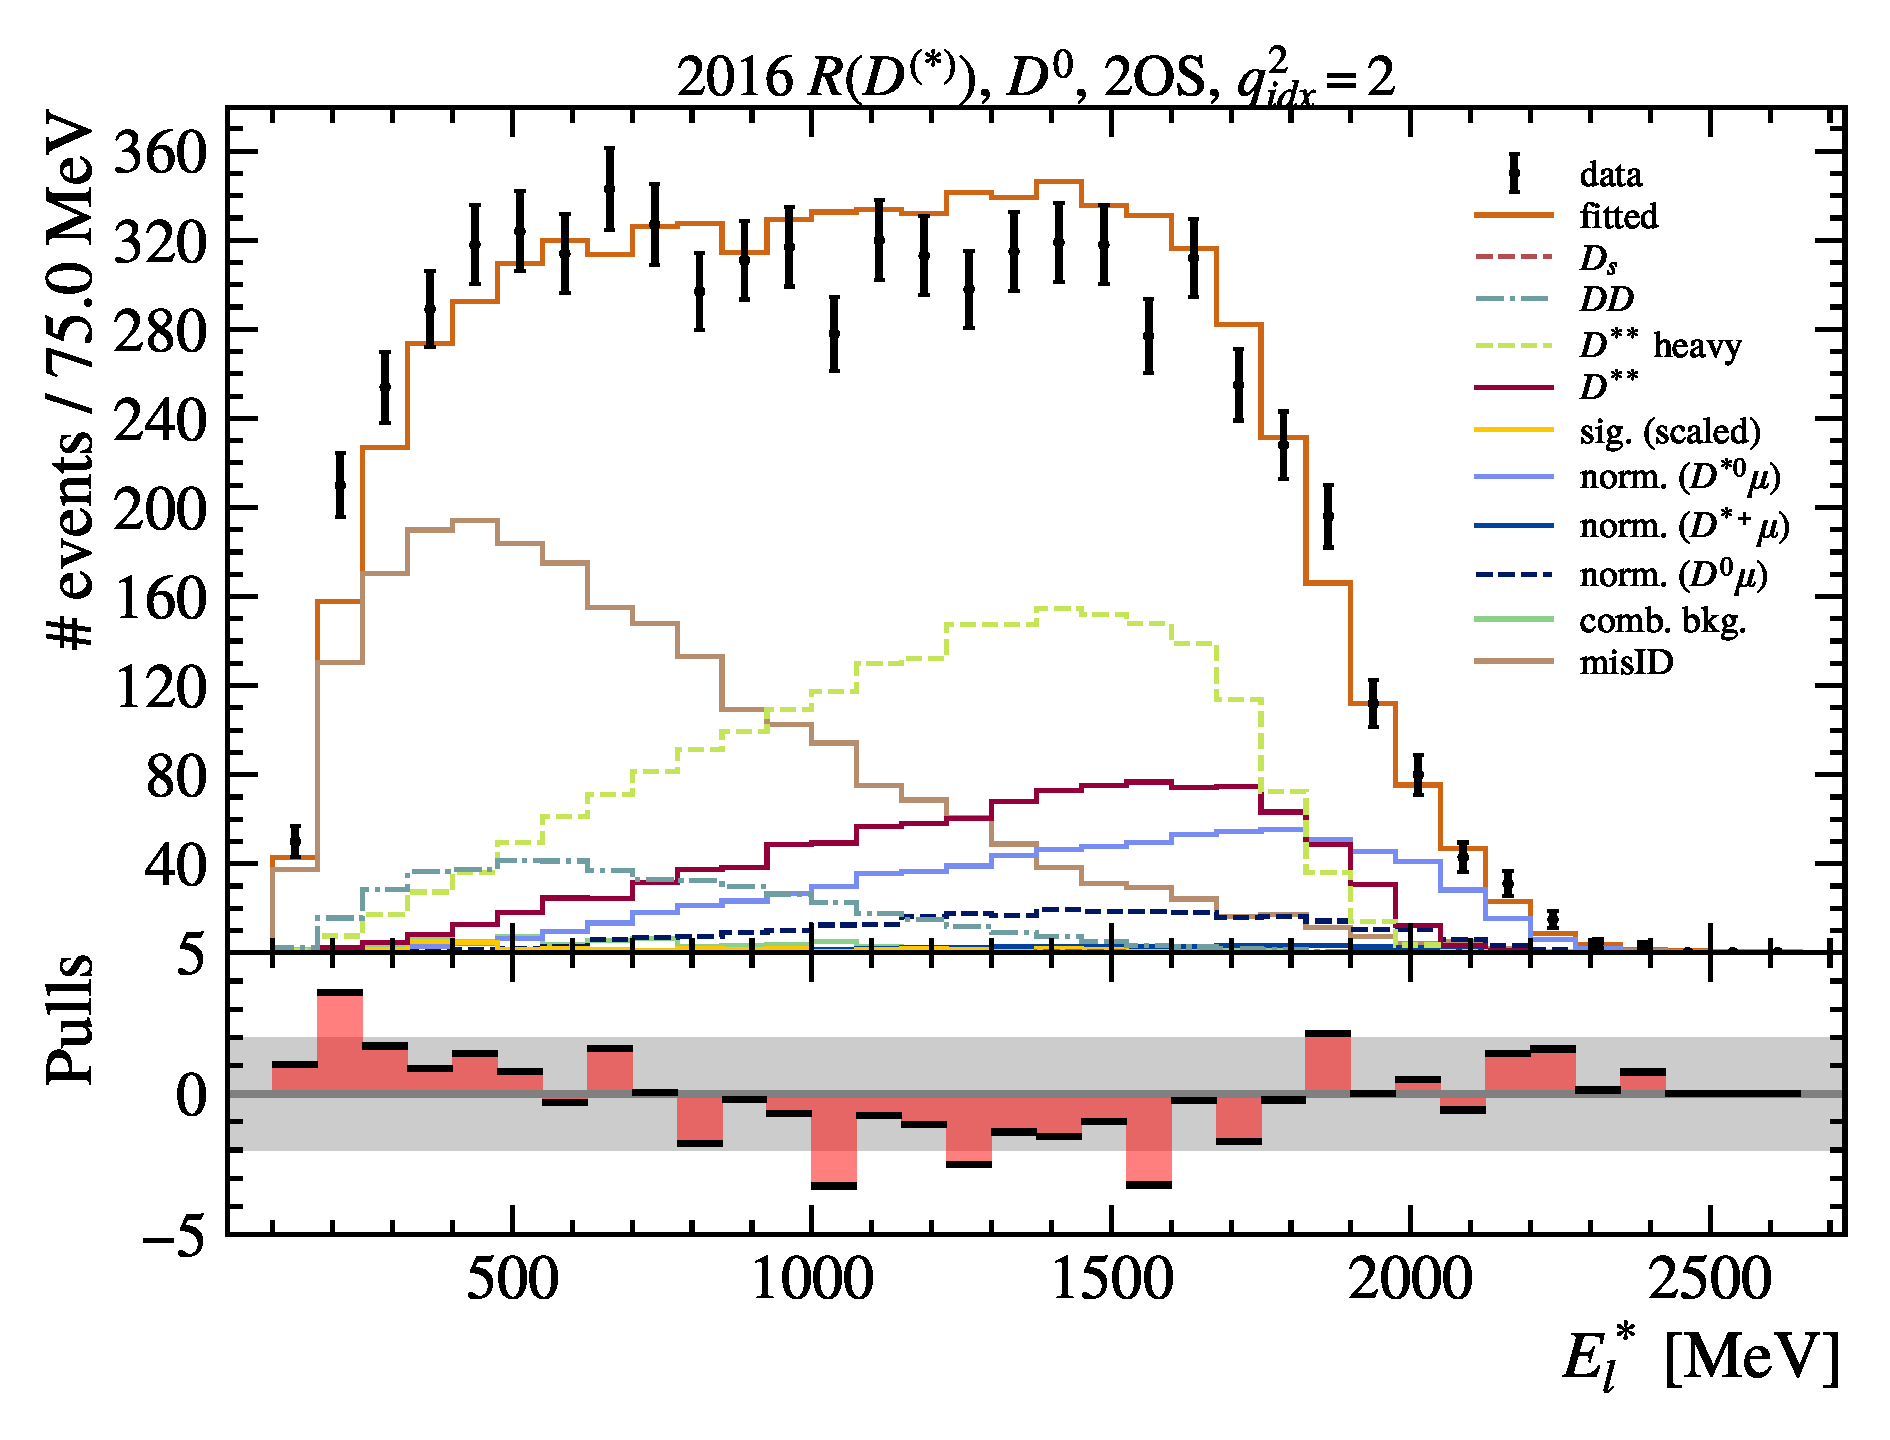
\includegraphics[width=0.24\textwidth]{./figs-fit-to-data/ctrl-fit/lines_q2_slices/fit_result-lines_q2_idx2-D0-2os-el.pdf}
    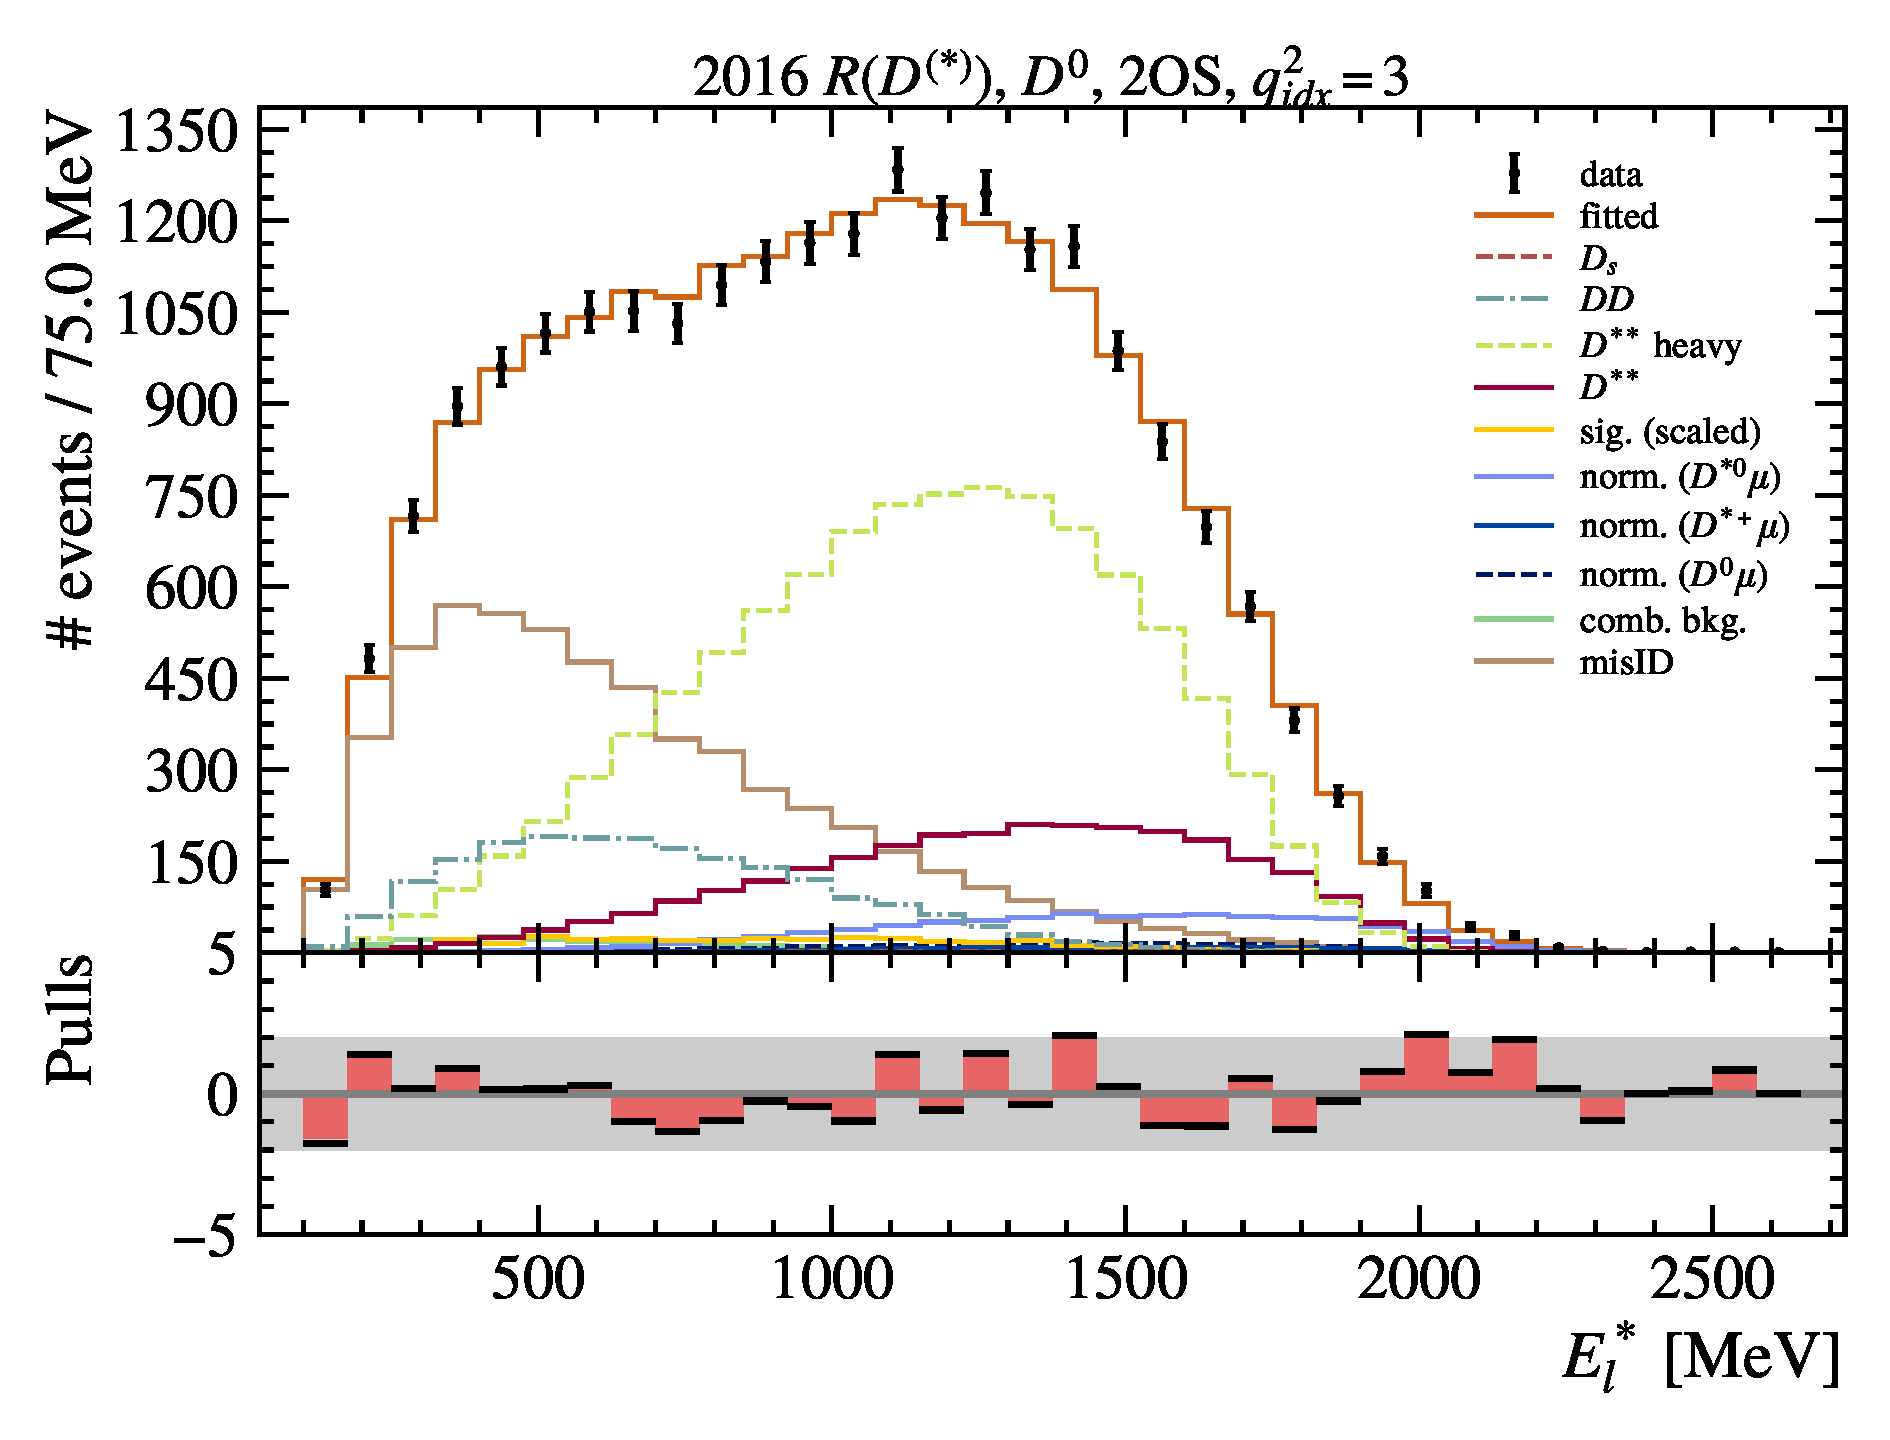
\includegraphics[width=0.24\textwidth]{./figs-fit-to-data/ctrl-fit/lines_q2_slices/fit_result-lines_q2_idx3-D0-2os-el.pdf}
    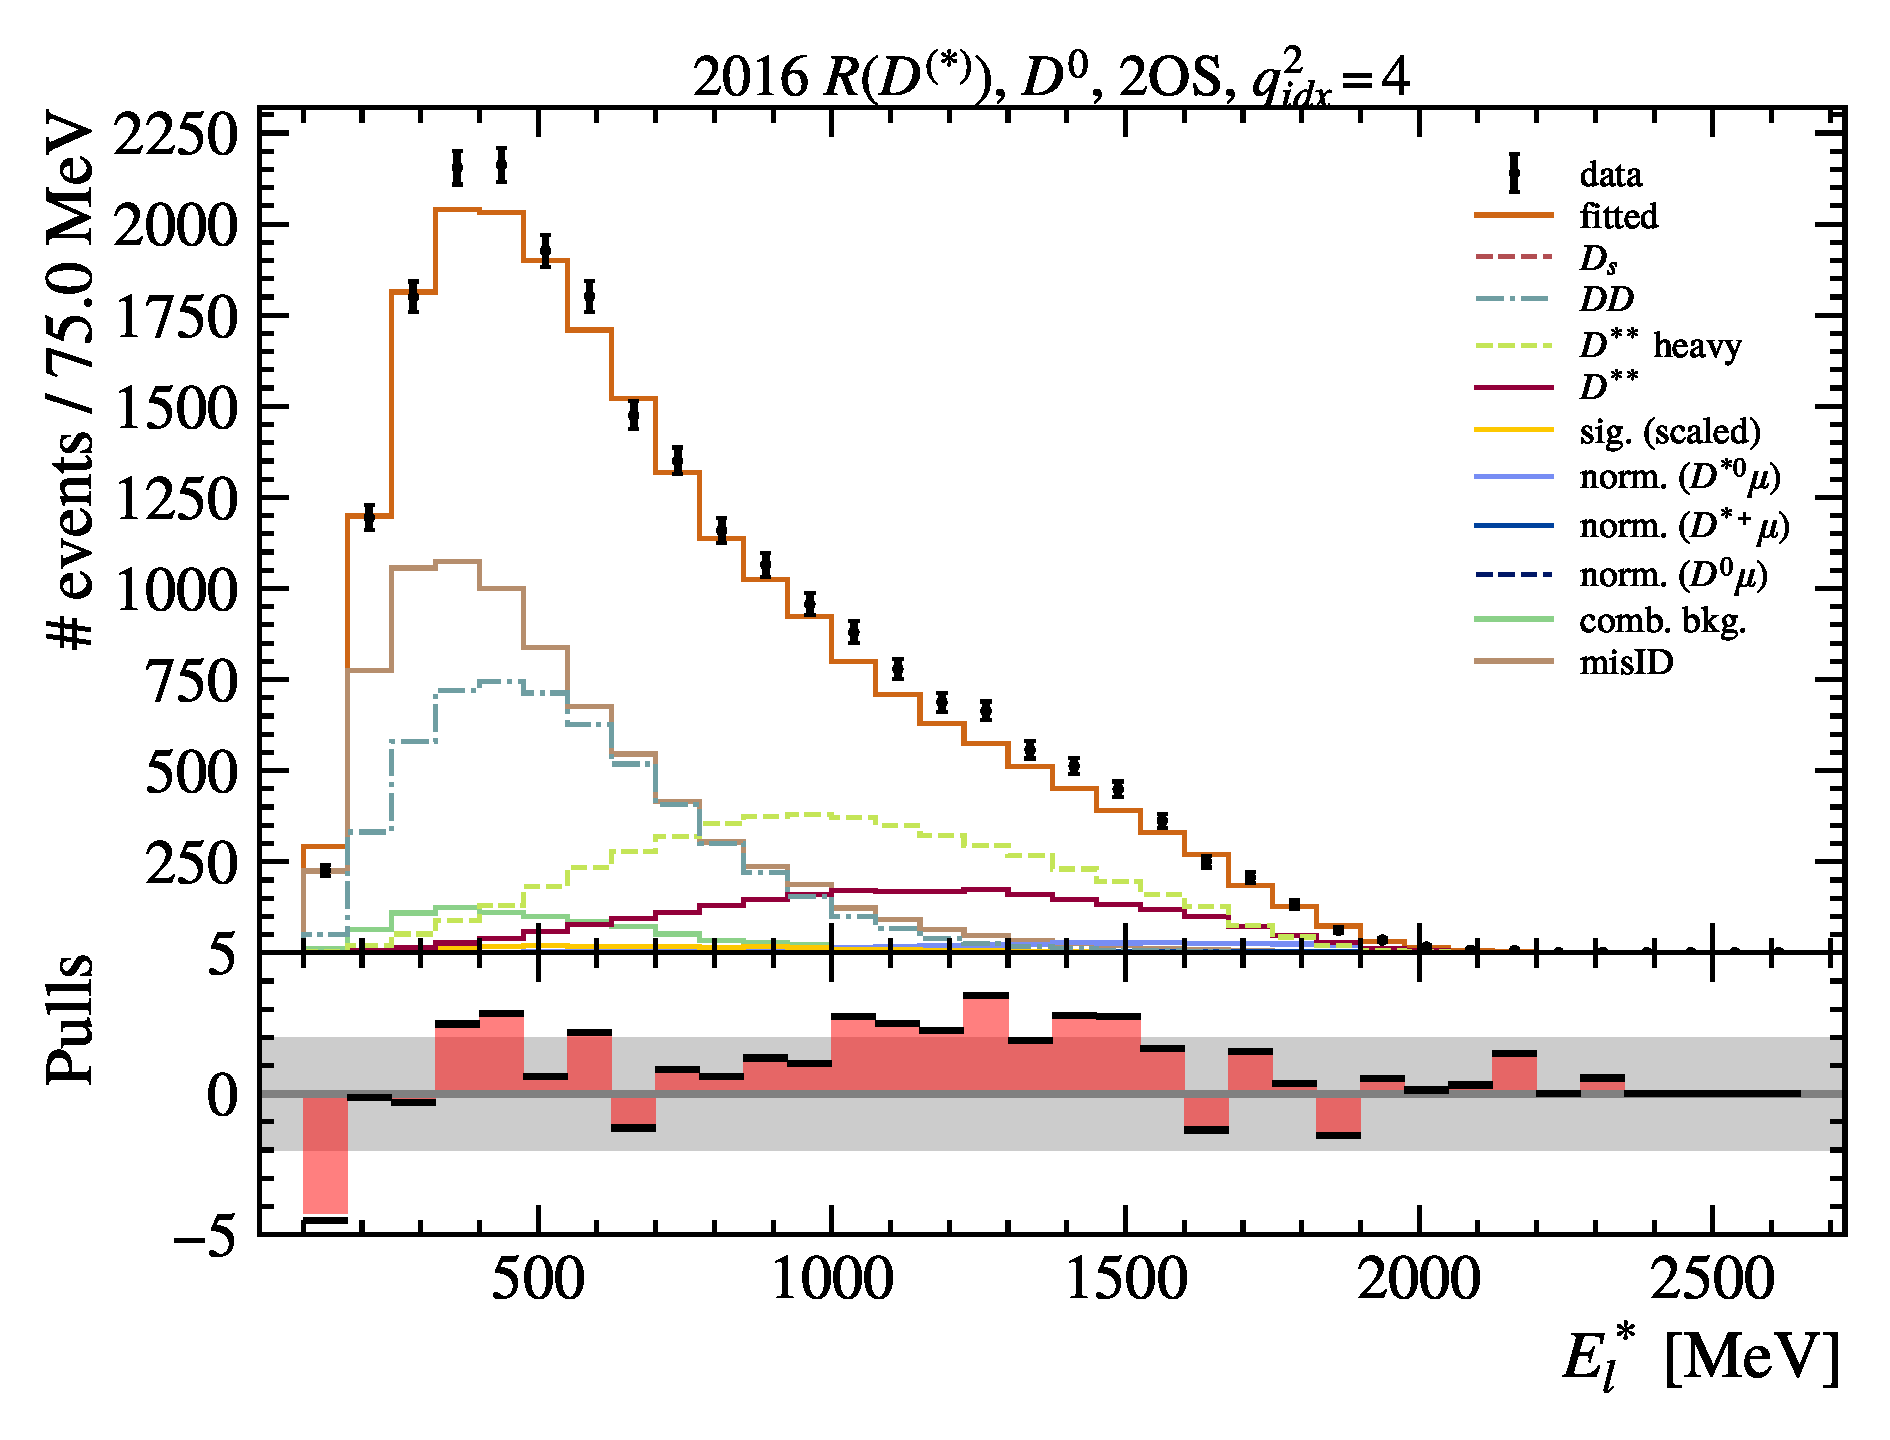
\includegraphics[width=0.24\textwidth]{./figs-fit-to-data/ctrl-fit/lines_q2_slices/fit_result-lines_q2_idx4-D0-2os-el.pdf}

    \caption{Control fit for 2OS sample, \Dz channel.}
    \label{fig:ctrl-2os-d0}
\end{figure}

\begin{figure}[htb]
    \centering
    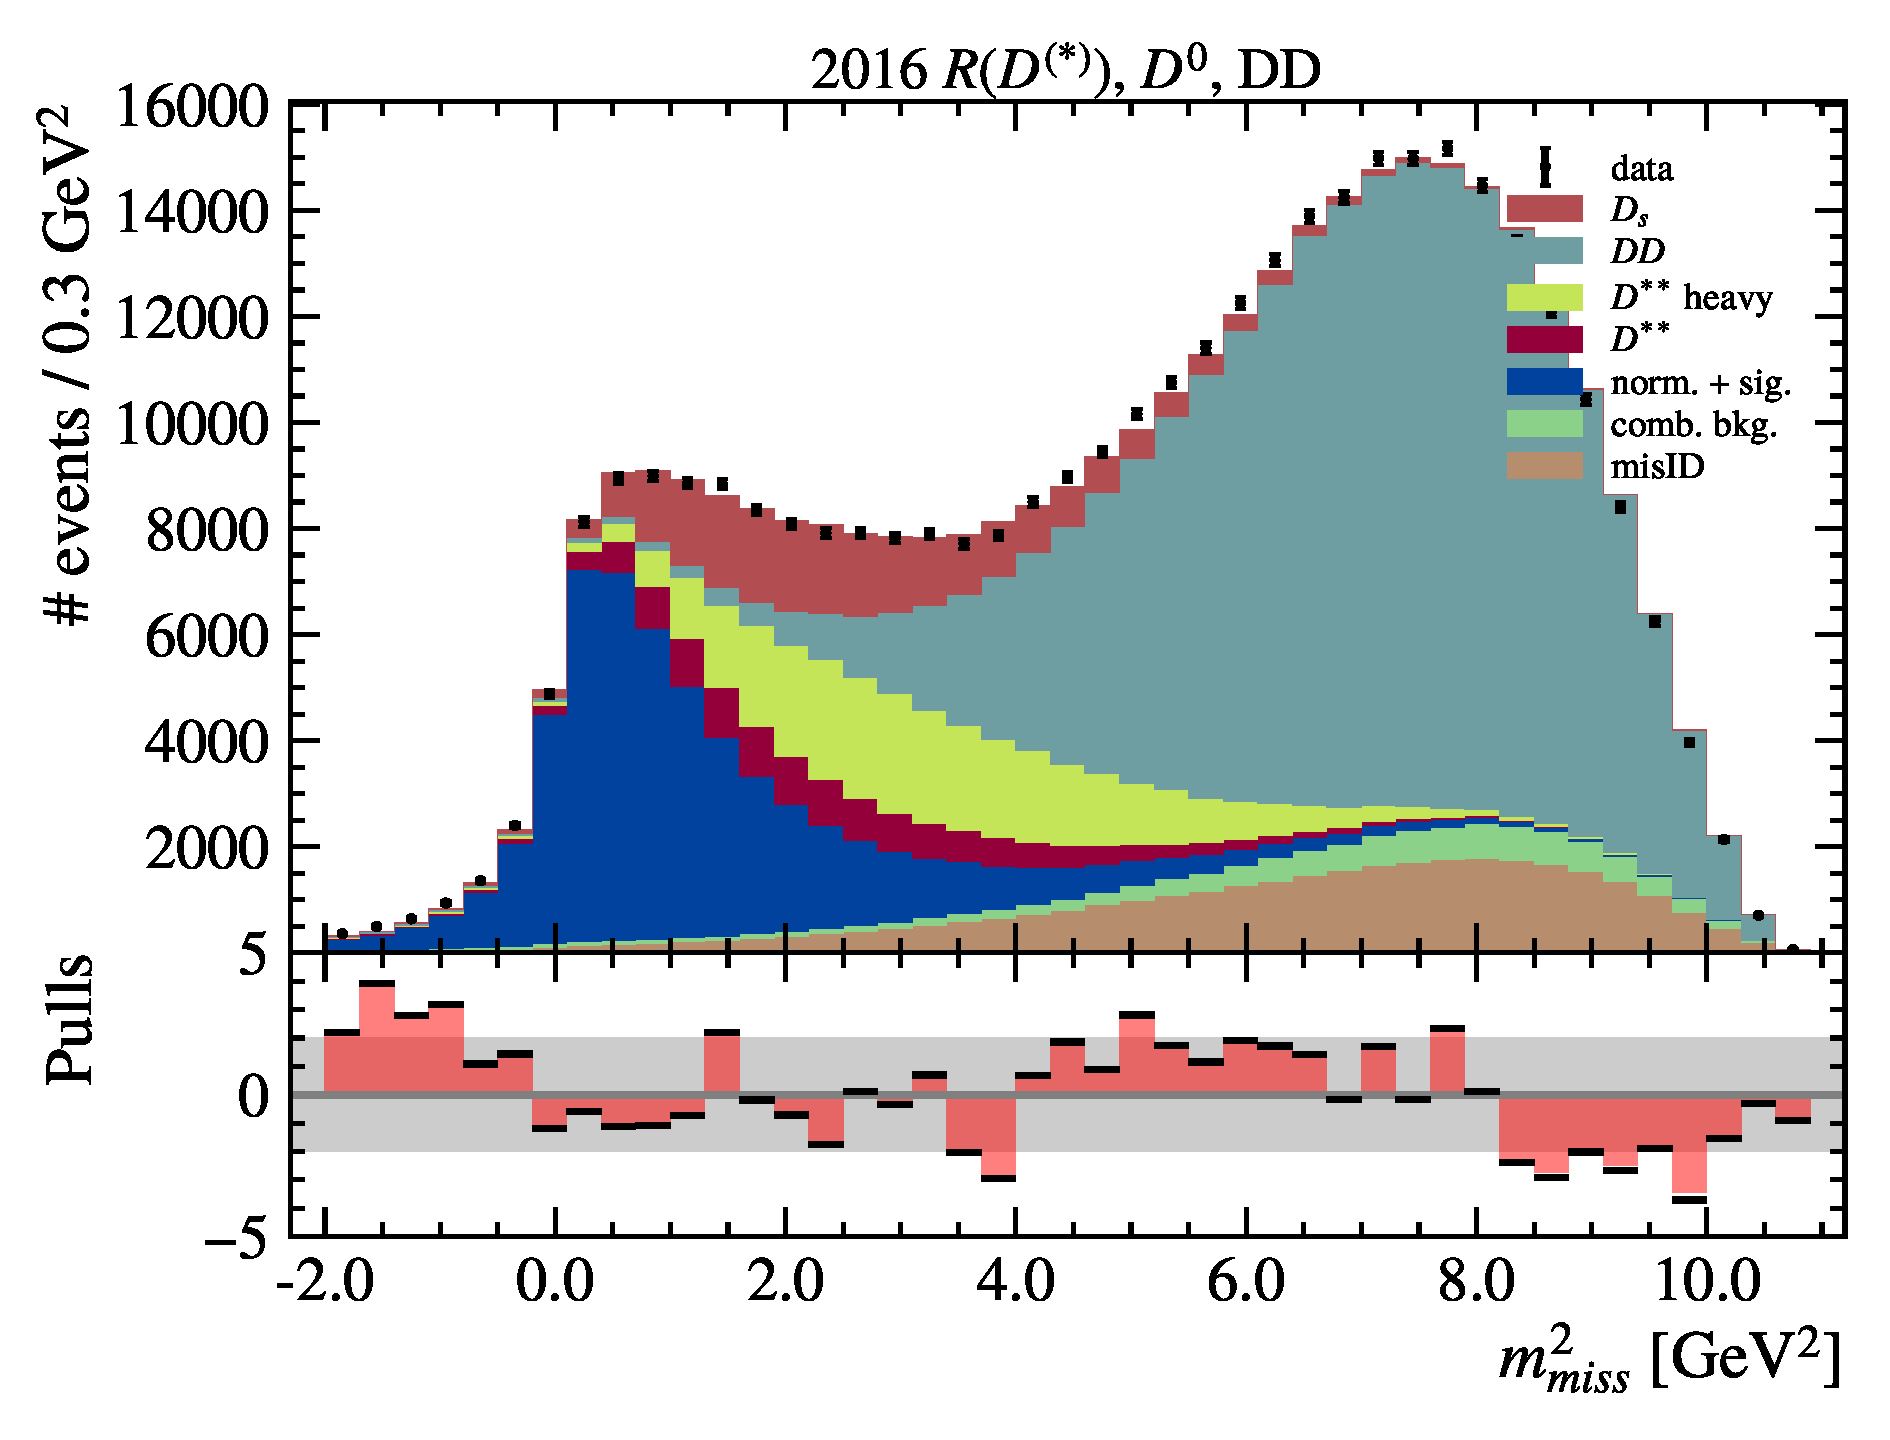
\includegraphics[width=0.32\textwidth]{./figs-fit-to-data/ctrl-fit/stacked/fit_result-stacked-D0-dd-mmiss2.pdf}
    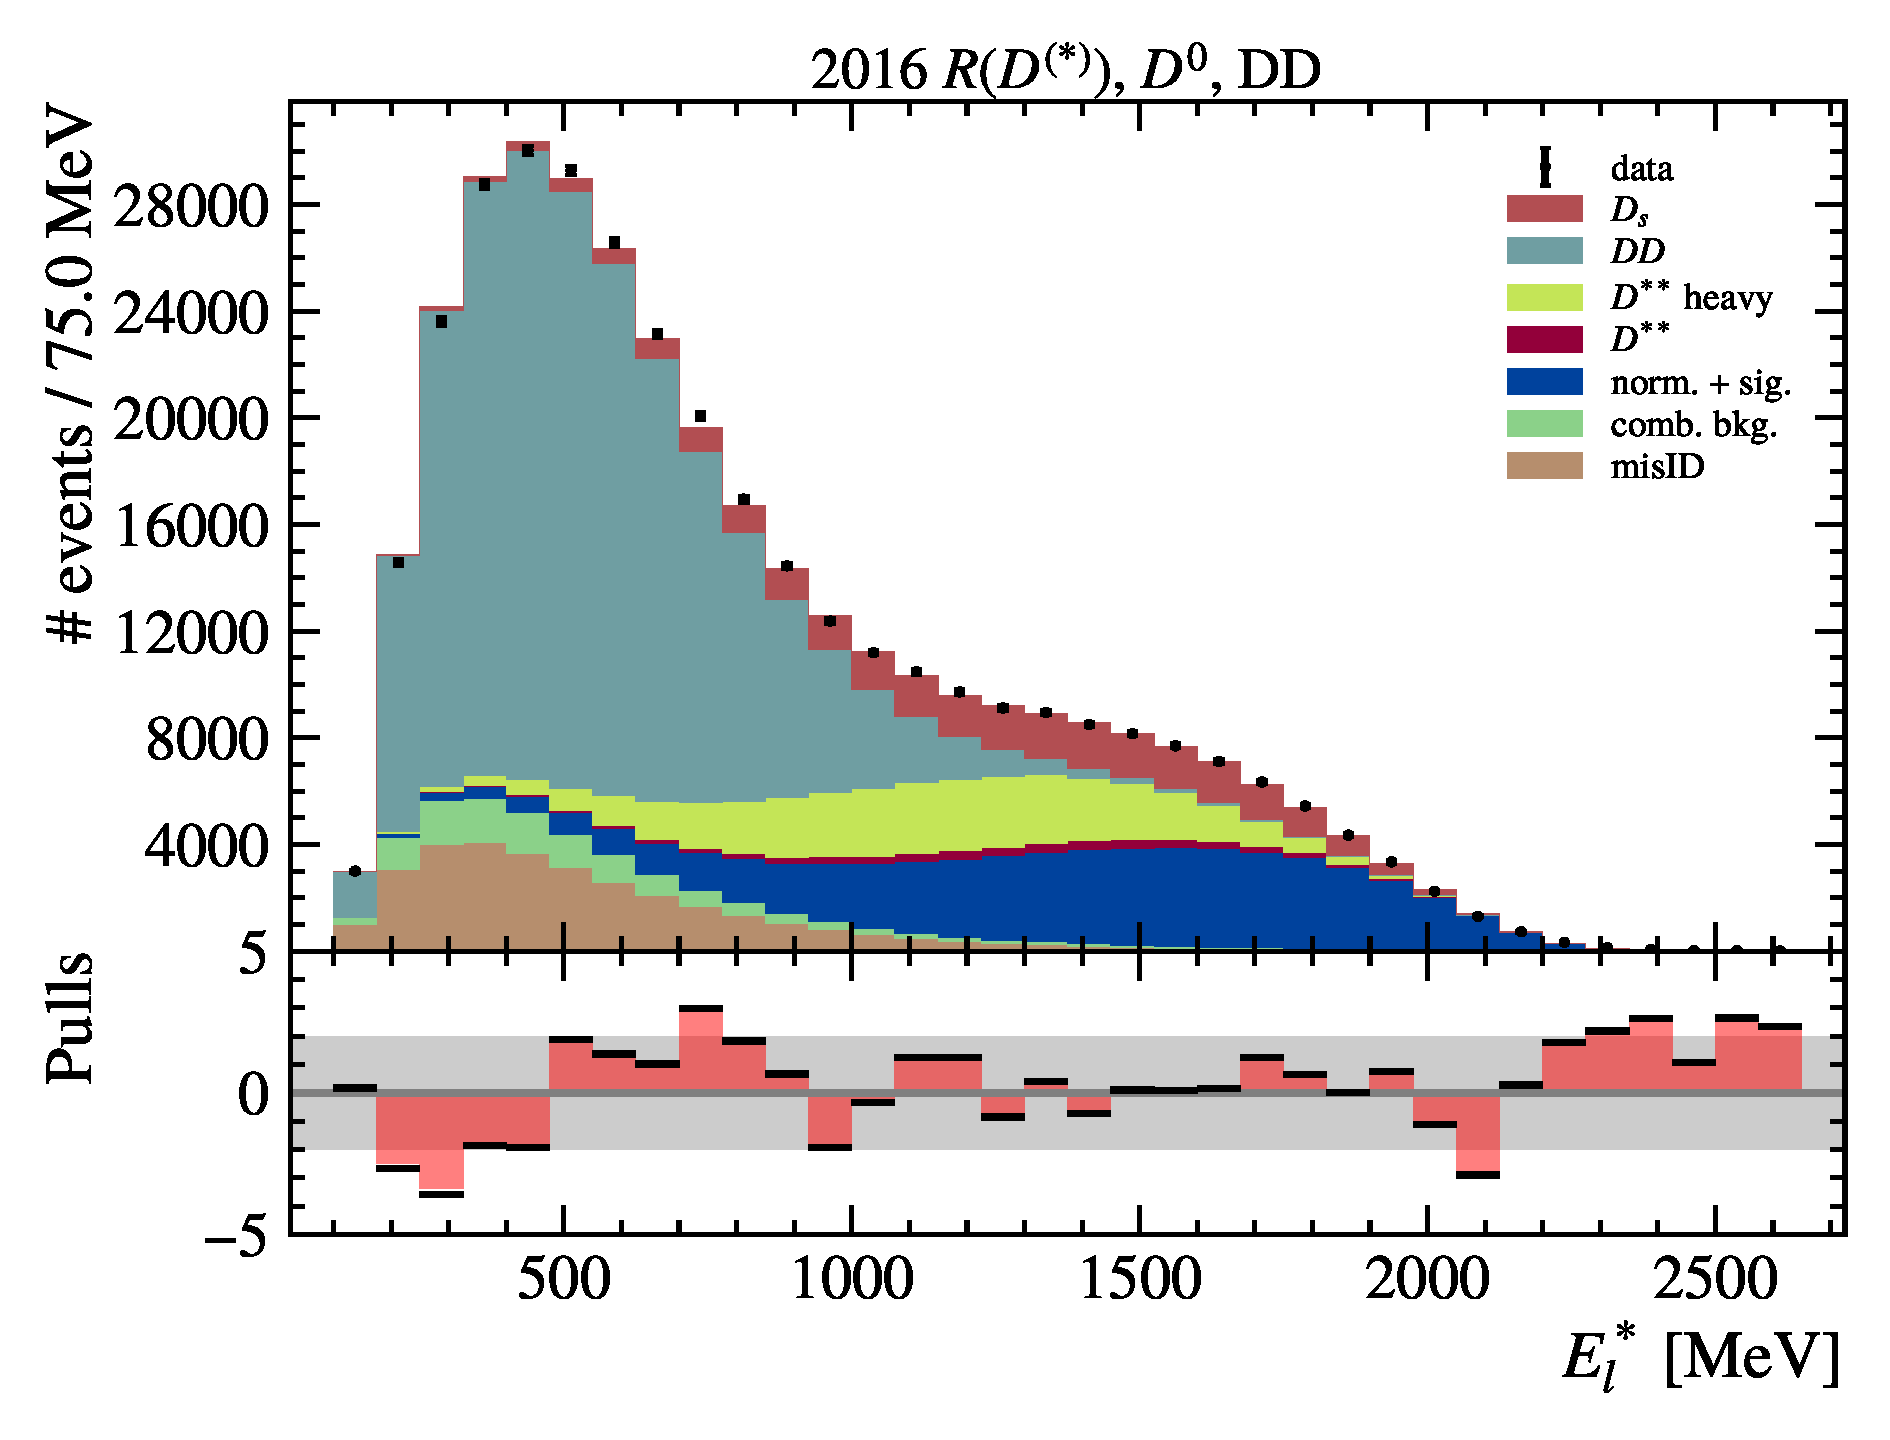
\includegraphics[width=0.32\textwidth]{./figs-fit-to-data/ctrl-fit/stacked/fit_result-stacked-D0-dd-el.pdf}
    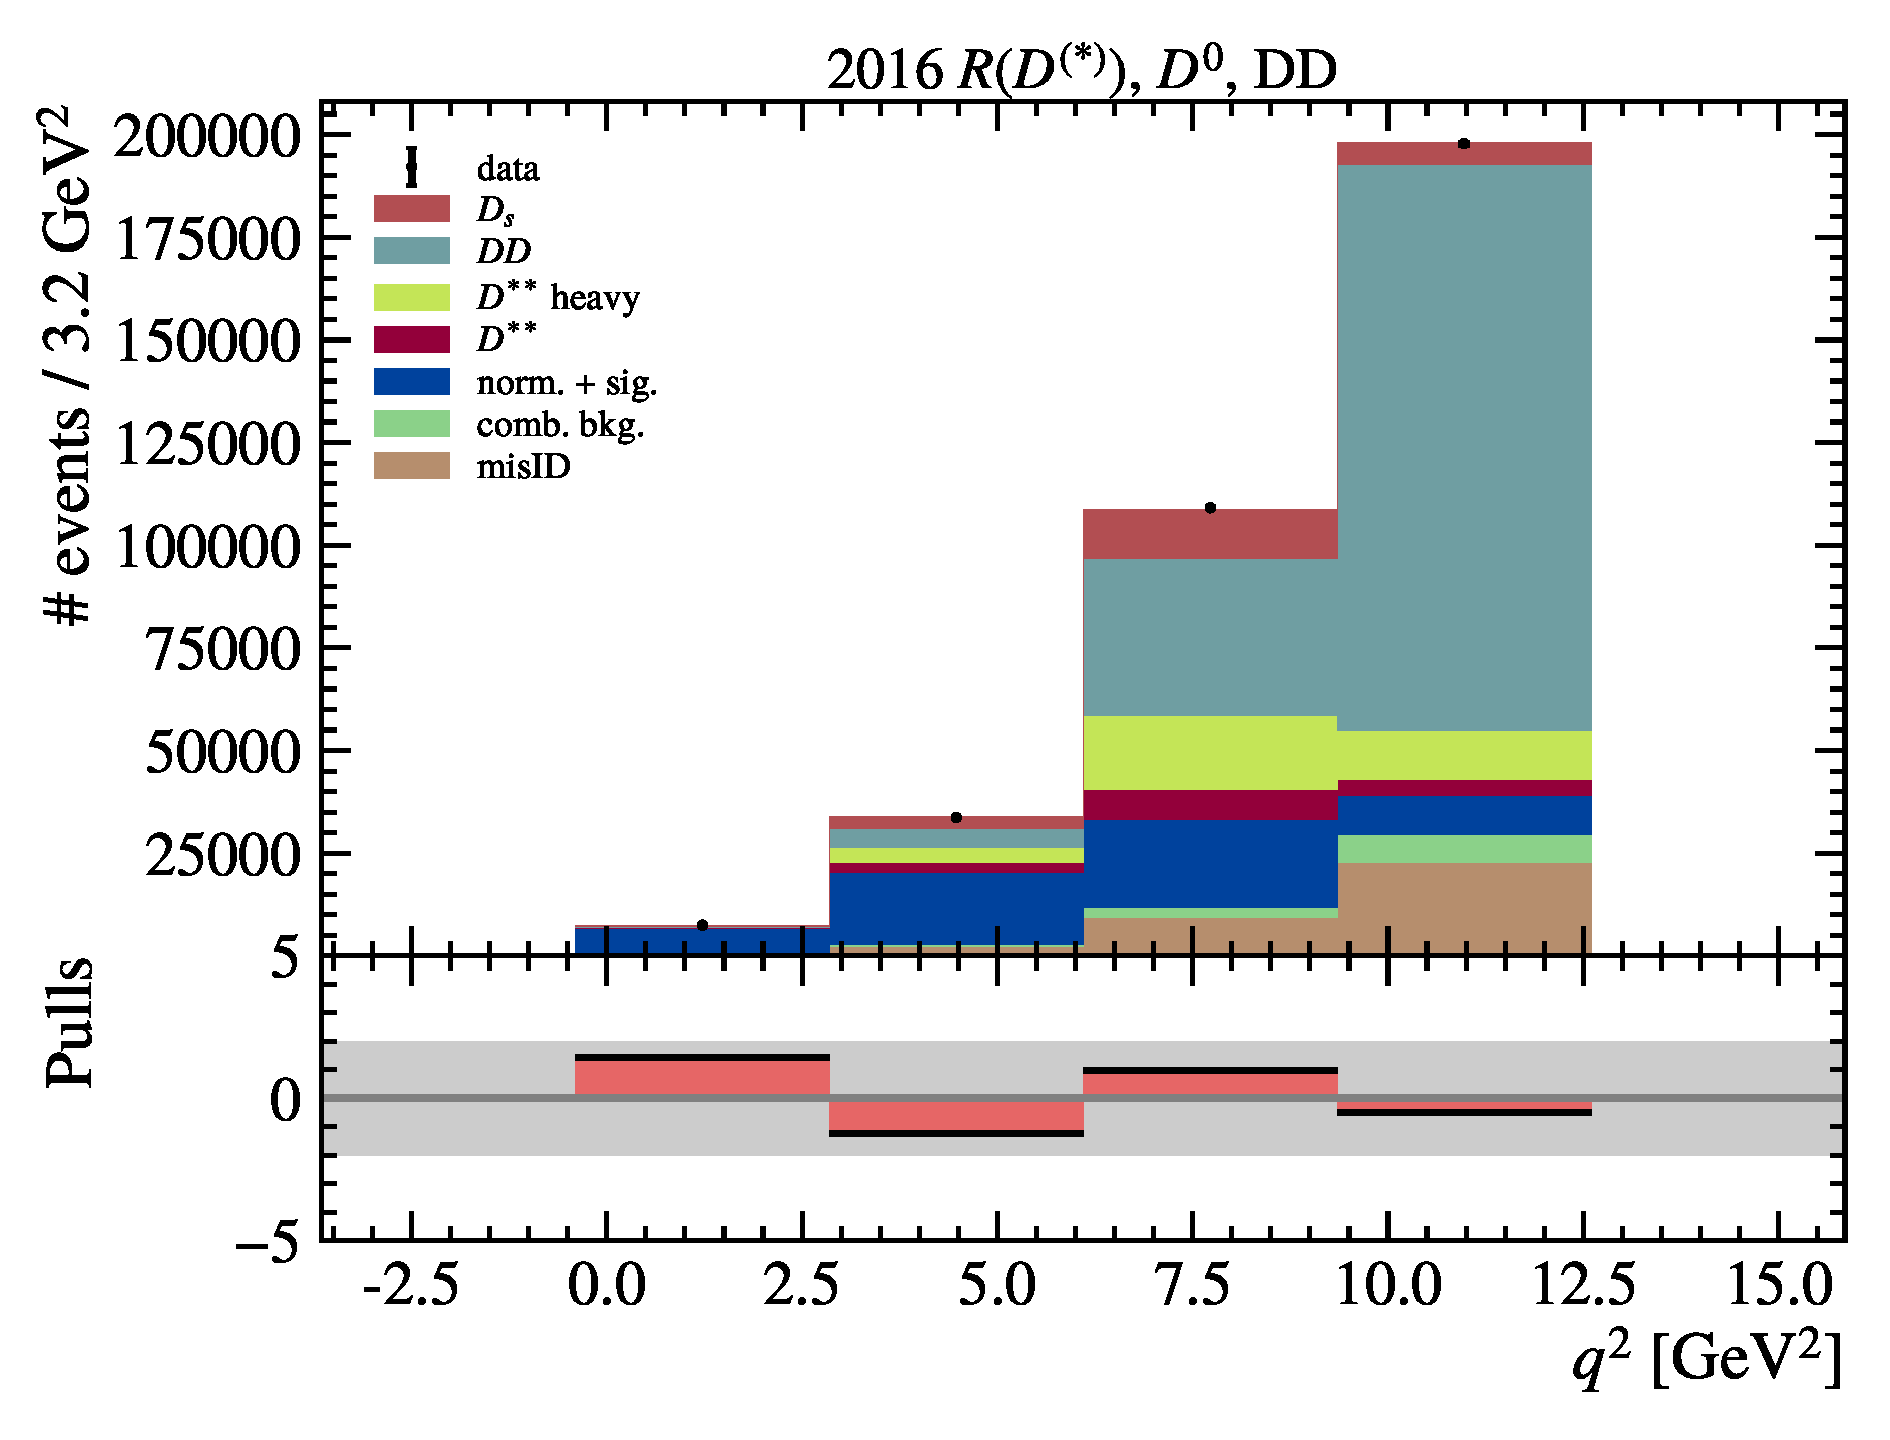
\includegraphics[width=0.32\textwidth]{./figs-fit-to-data/ctrl-fit/stacked/fit_result-stacked-D0-dd-q2.pdf}

    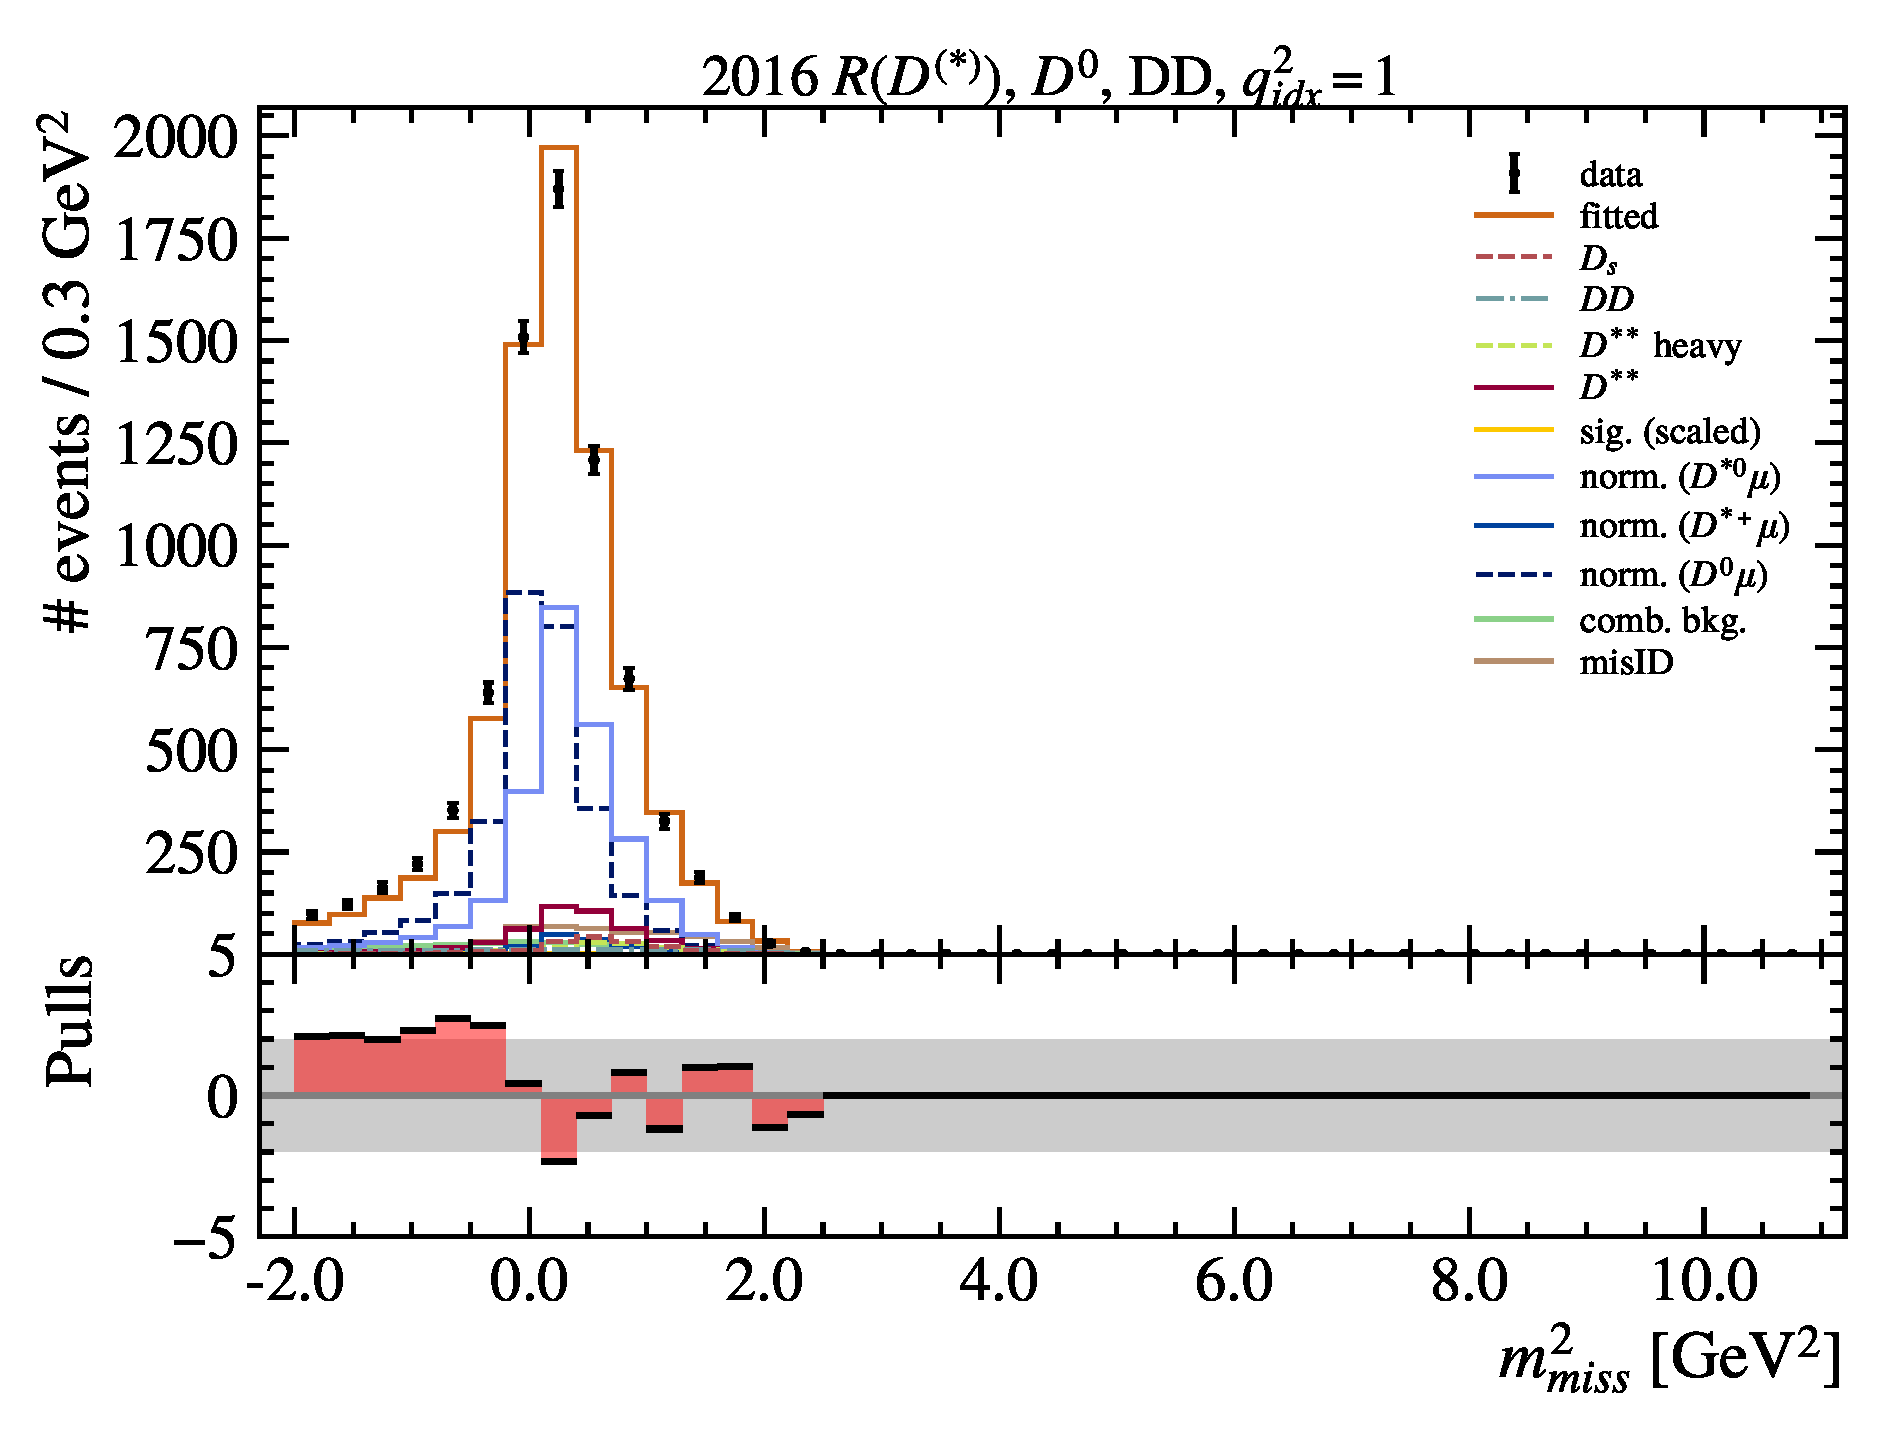
\includegraphics[width=0.24\textwidth]{./figs-fit-to-data/ctrl-fit/lines_q2_slices/fit_result-lines_q2_idx1-D0-dd-mmiss2.pdf}
    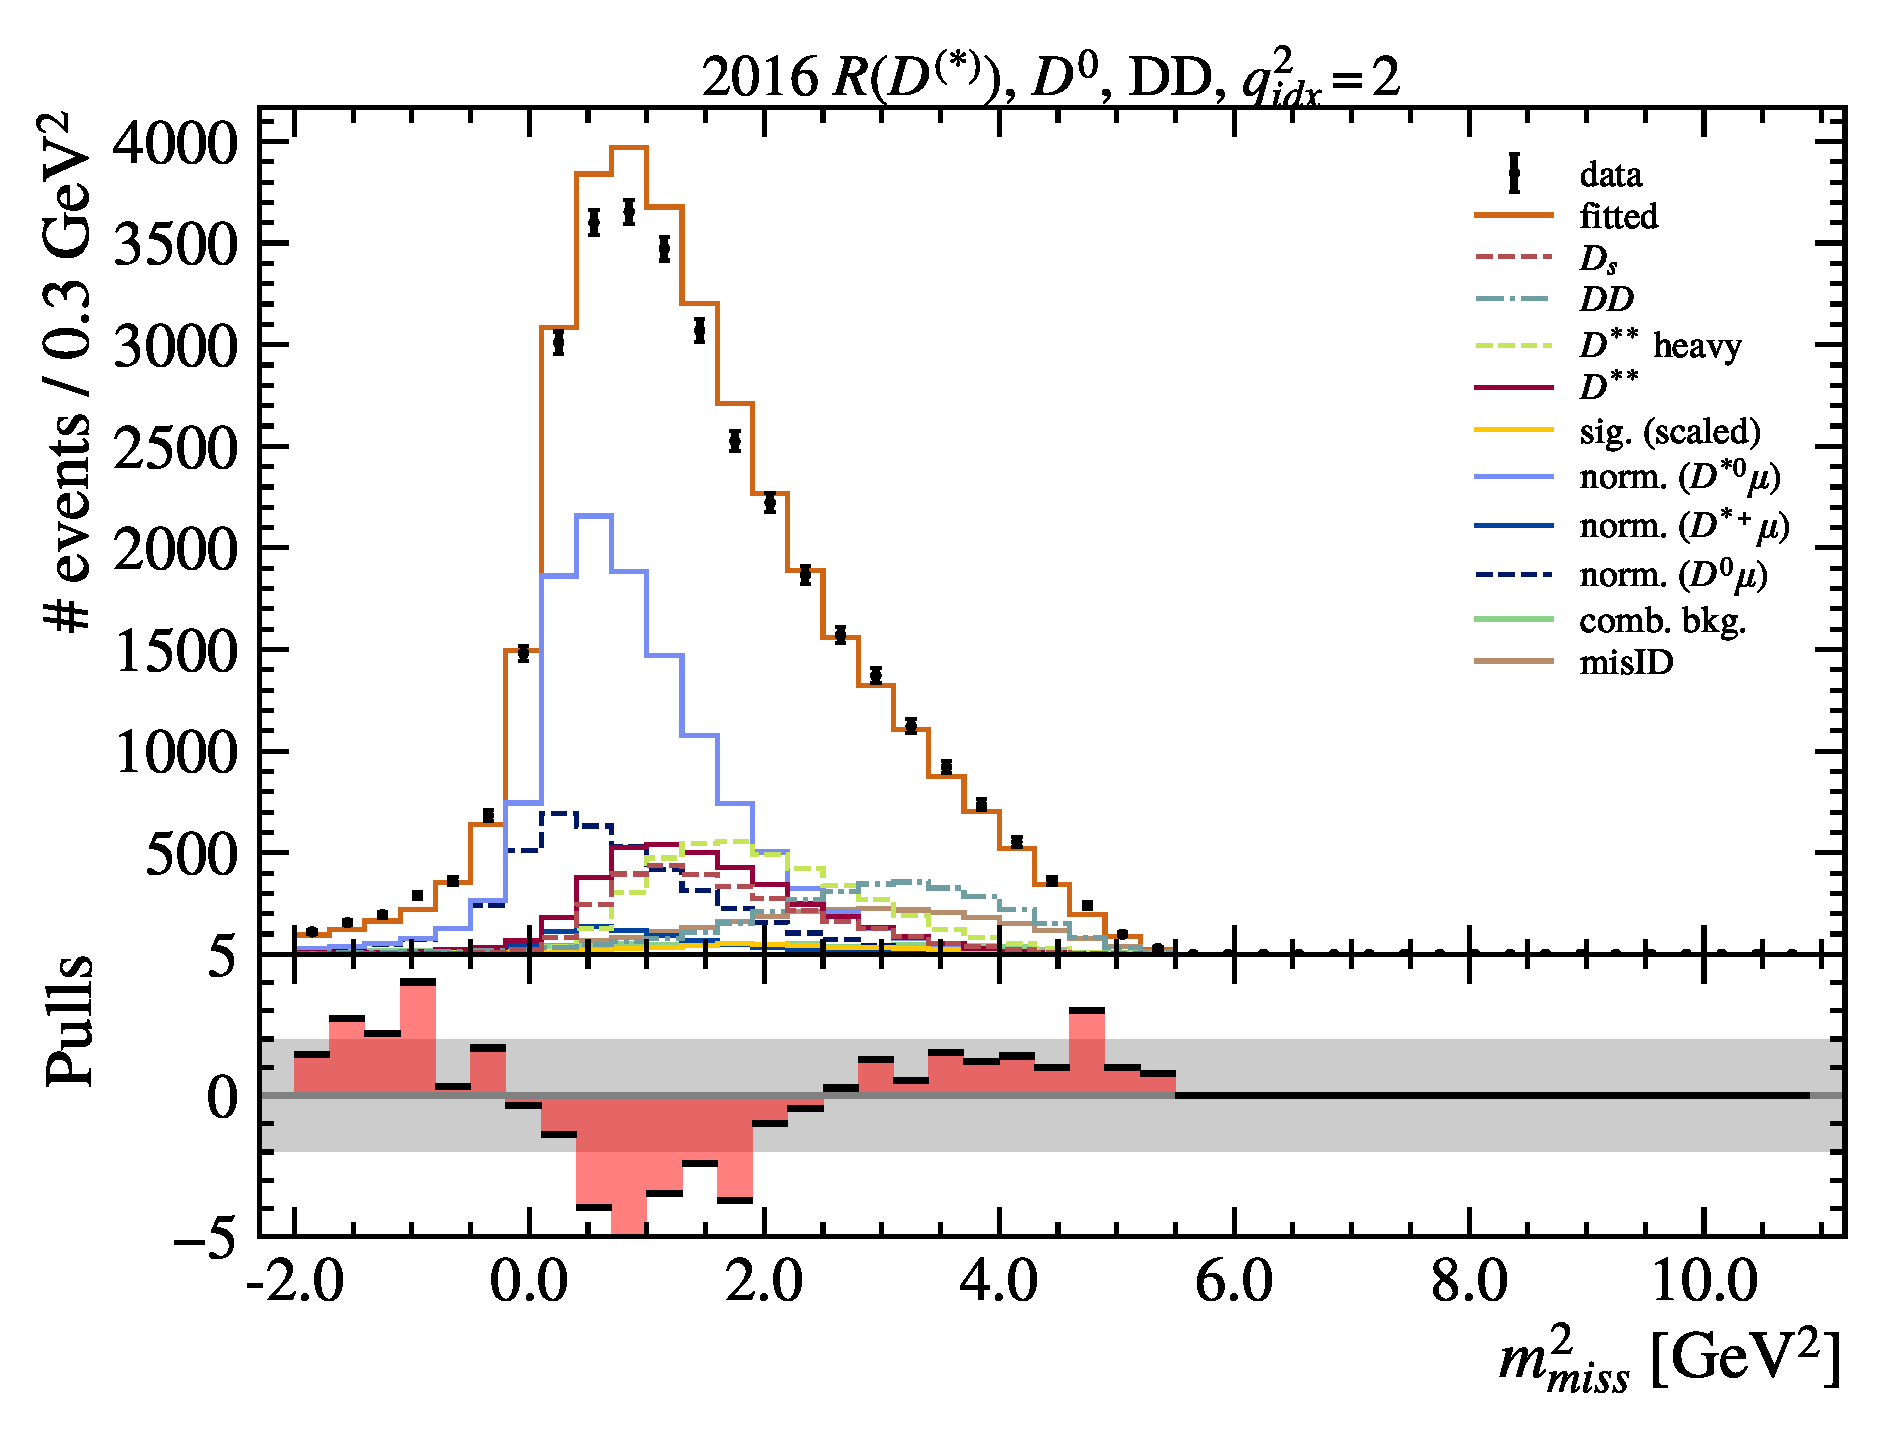
\includegraphics[width=0.24\textwidth]{./figs-fit-to-data/ctrl-fit/lines_q2_slices/fit_result-lines_q2_idx2-D0-dd-mmiss2.pdf}
    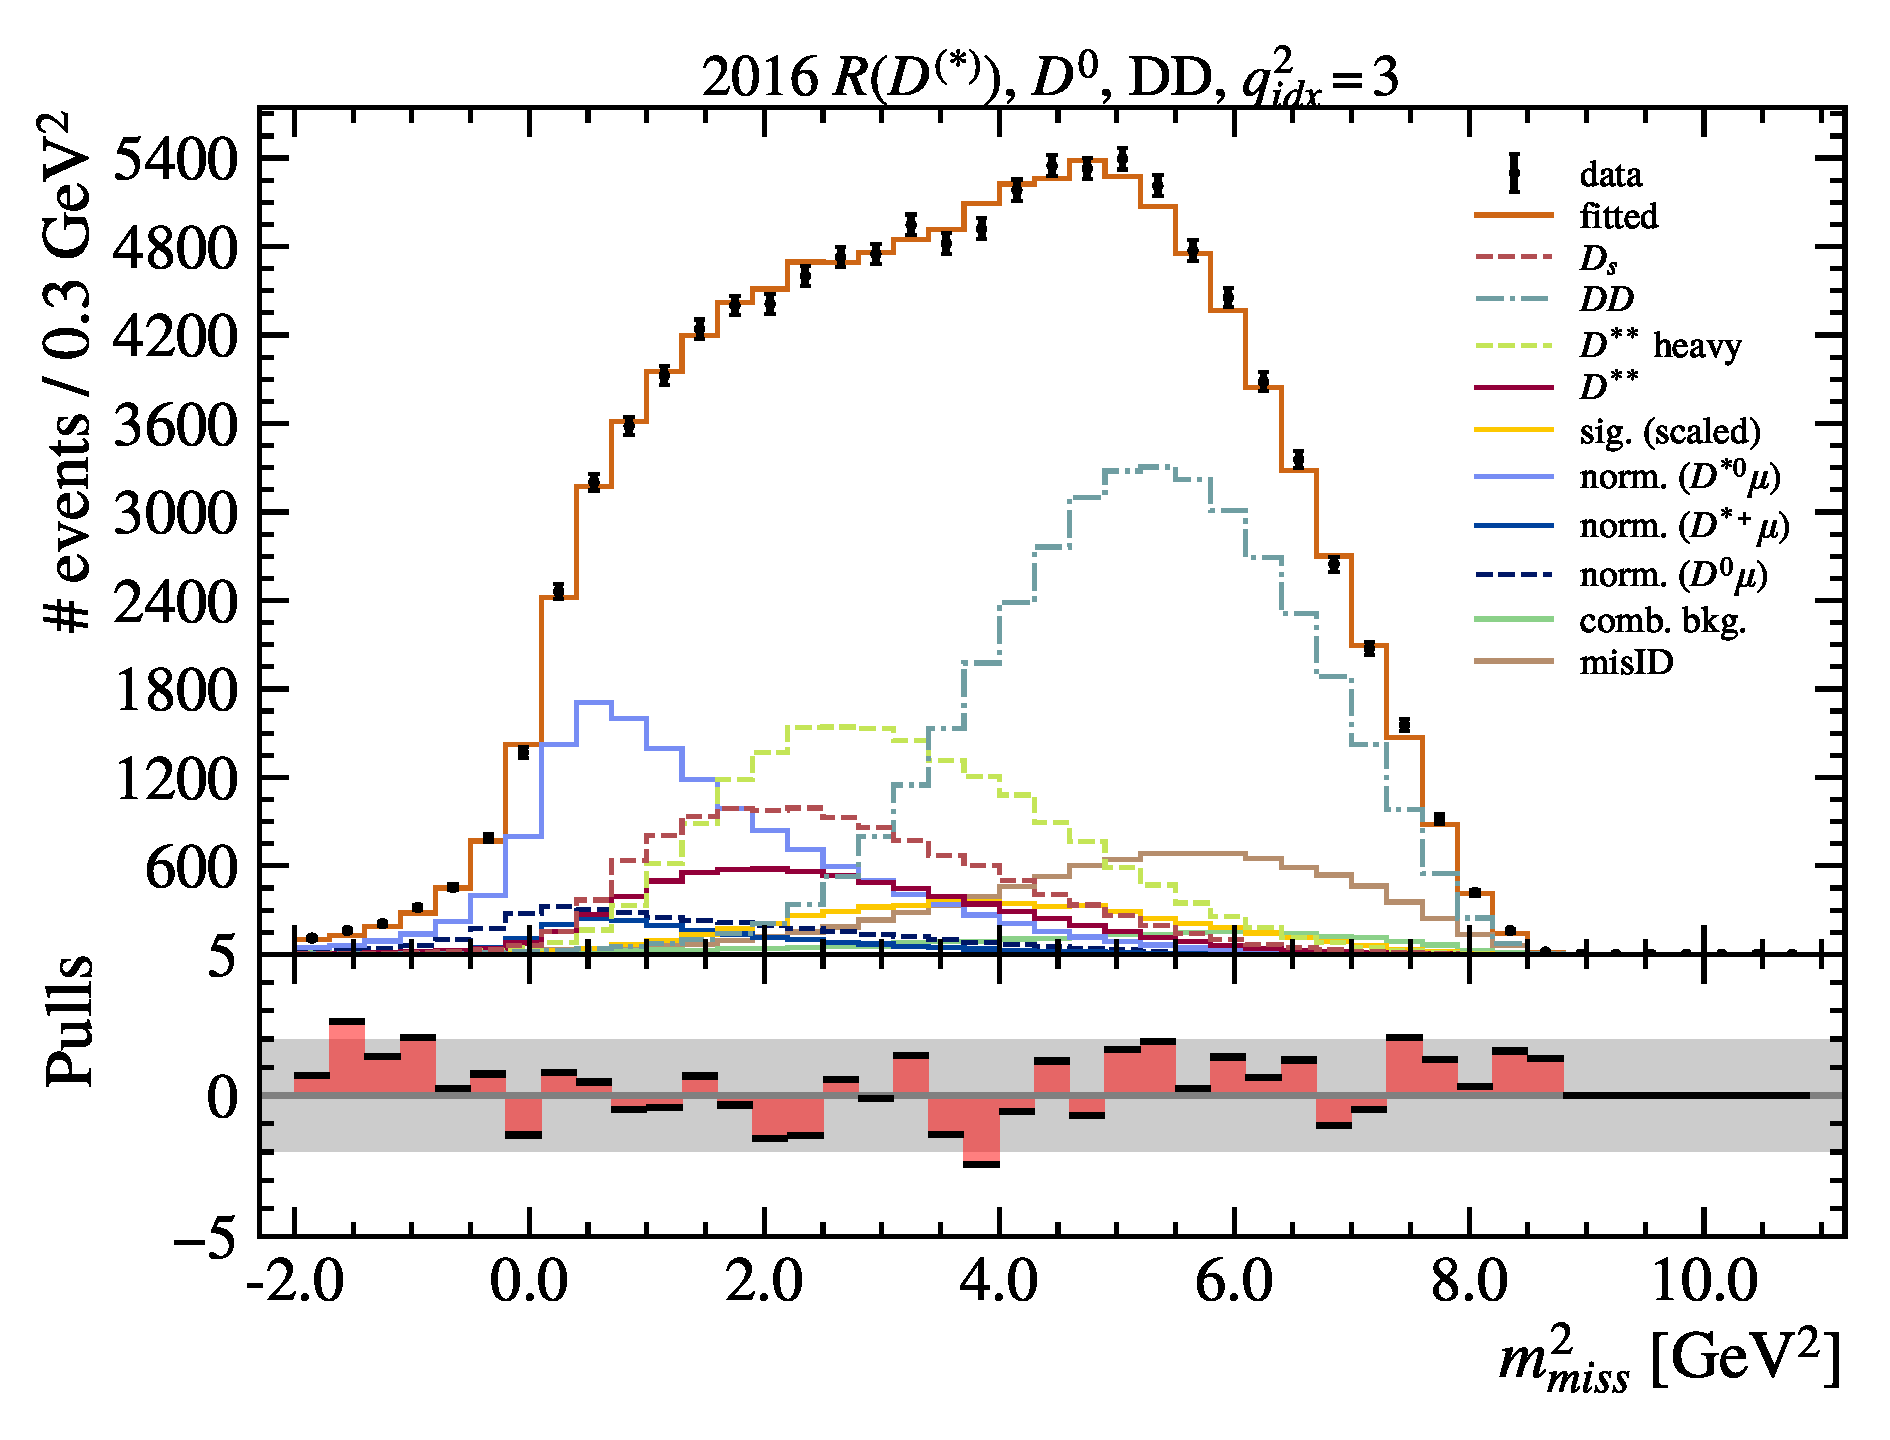
\includegraphics[width=0.24\textwidth]{./figs-fit-to-data/ctrl-fit/lines_q2_slices/fit_result-lines_q2_idx3-D0-dd-mmiss2.pdf}
    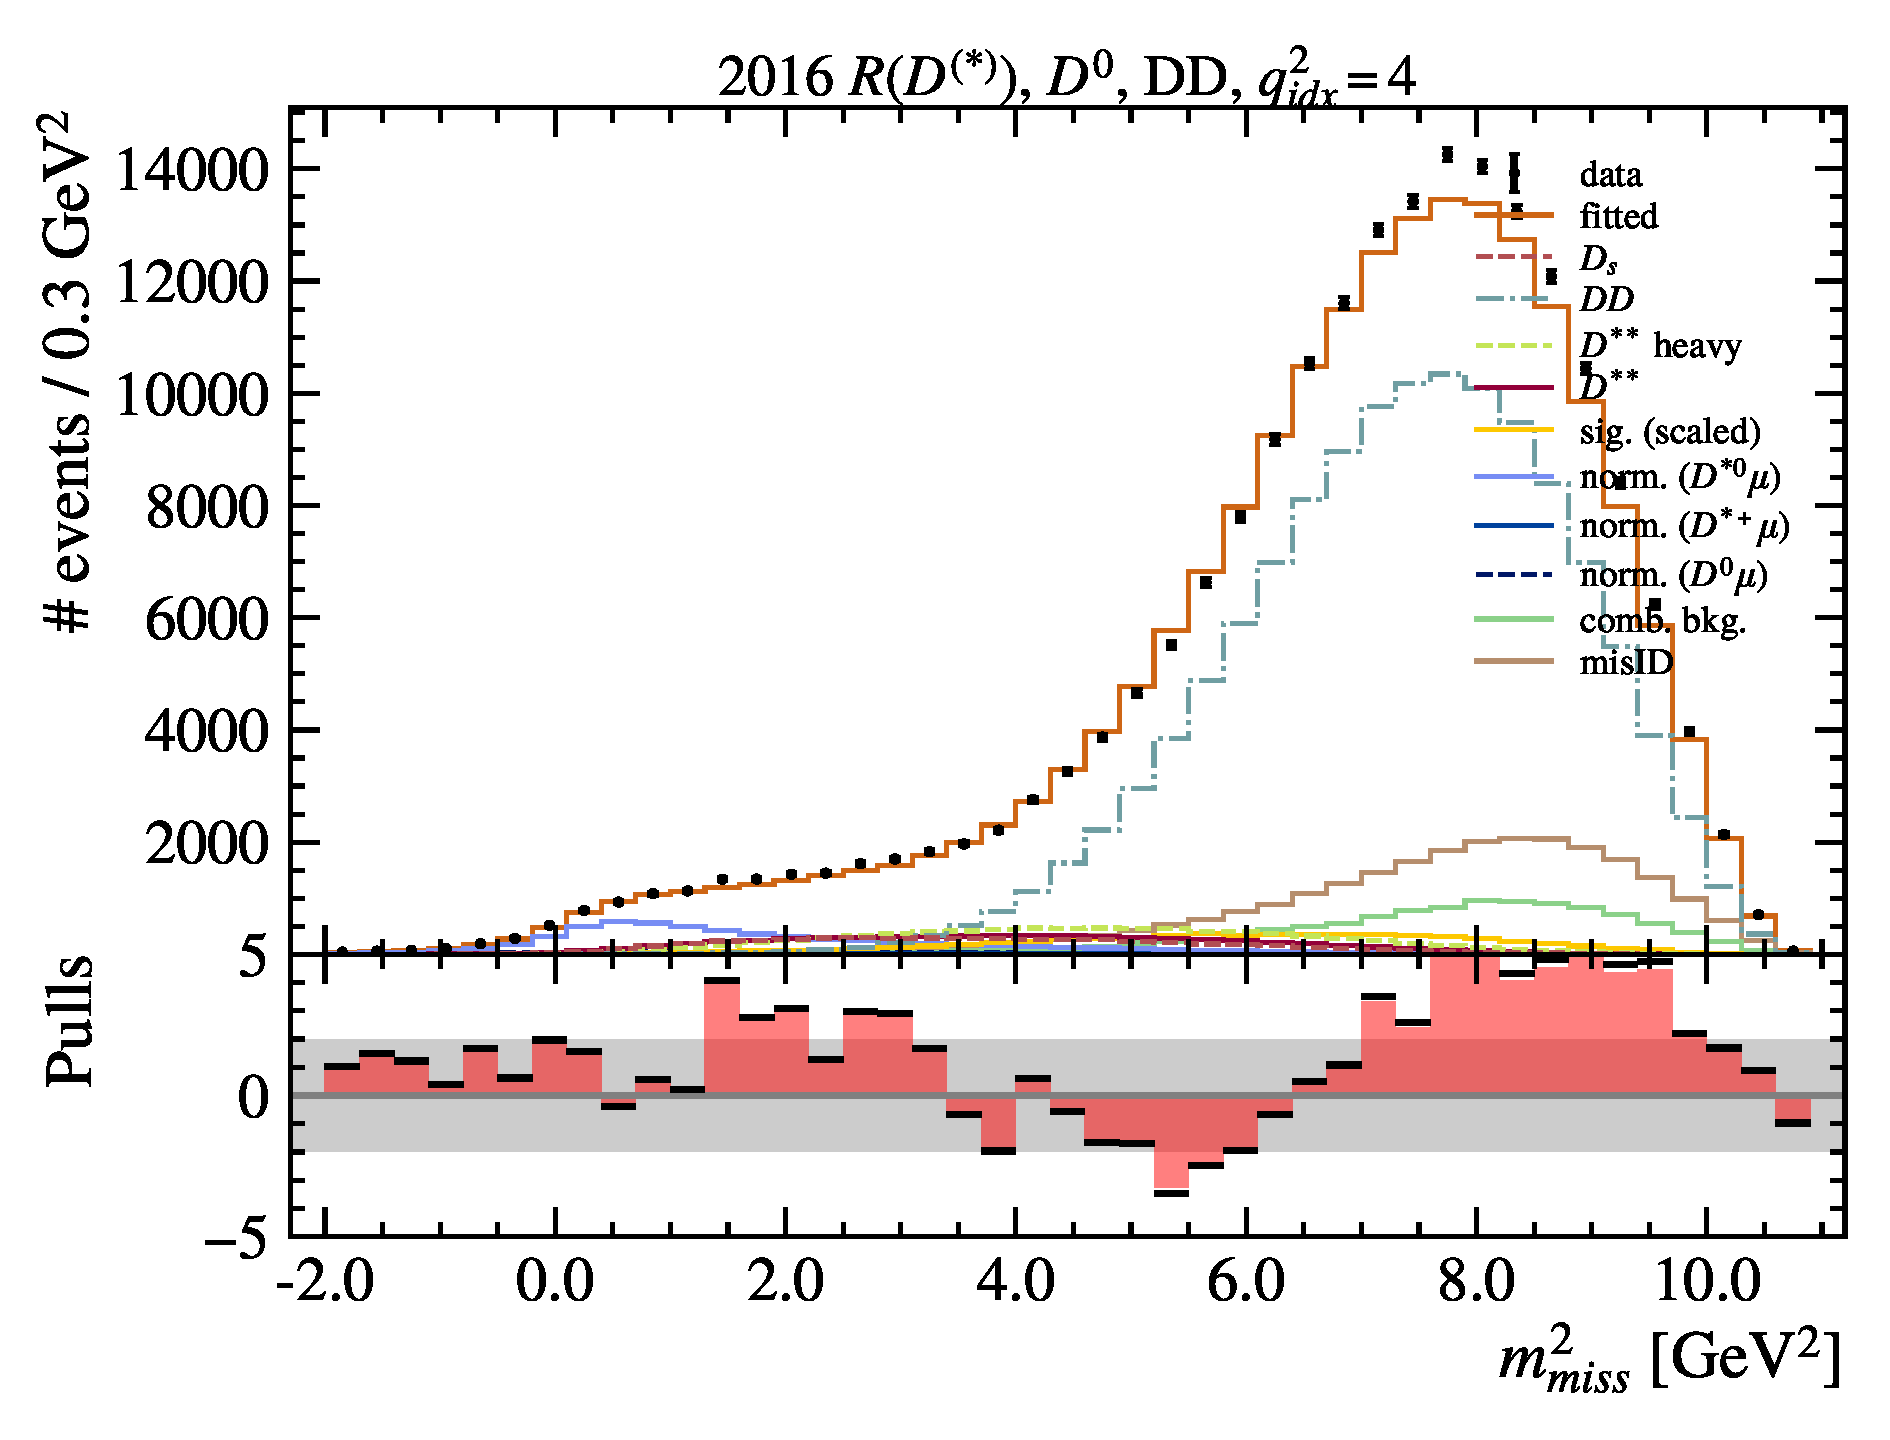
\includegraphics[width=0.24\textwidth]{./figs-fit-to-data/ctrl-fit/lines_q2_slices/fit_result-lines_q2_idx4-D0-dd-mmiss2.pdf}

    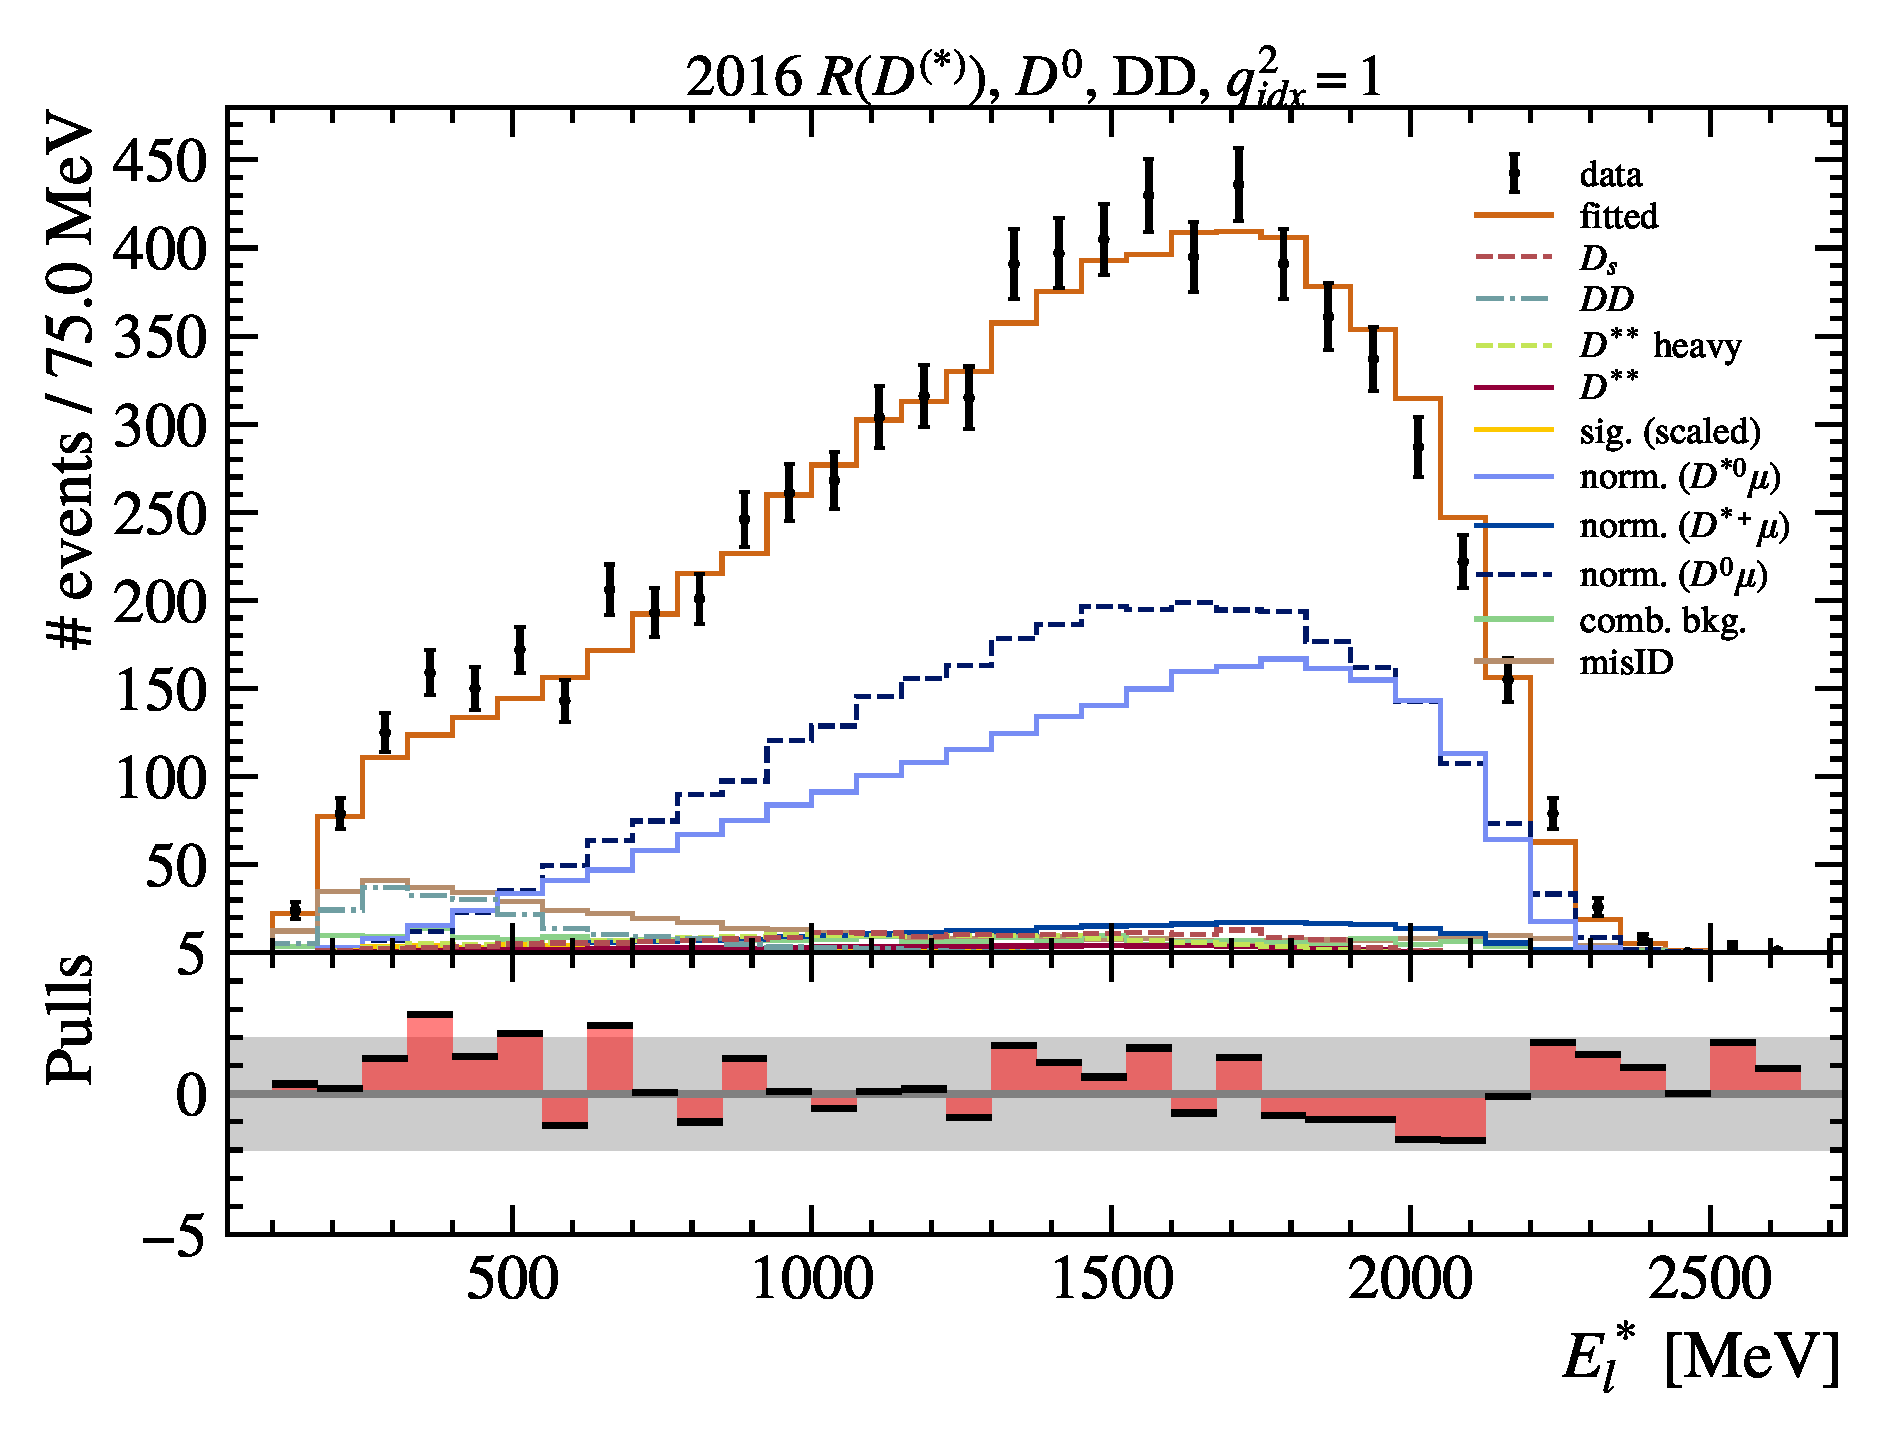
\includegraphics[width=0.24\textwidth]{./figs-fit-to-data/ctrl-fit/lines_q2_slices/fit_result-lines_q2_idx1-D0-dd-el.pdf}
    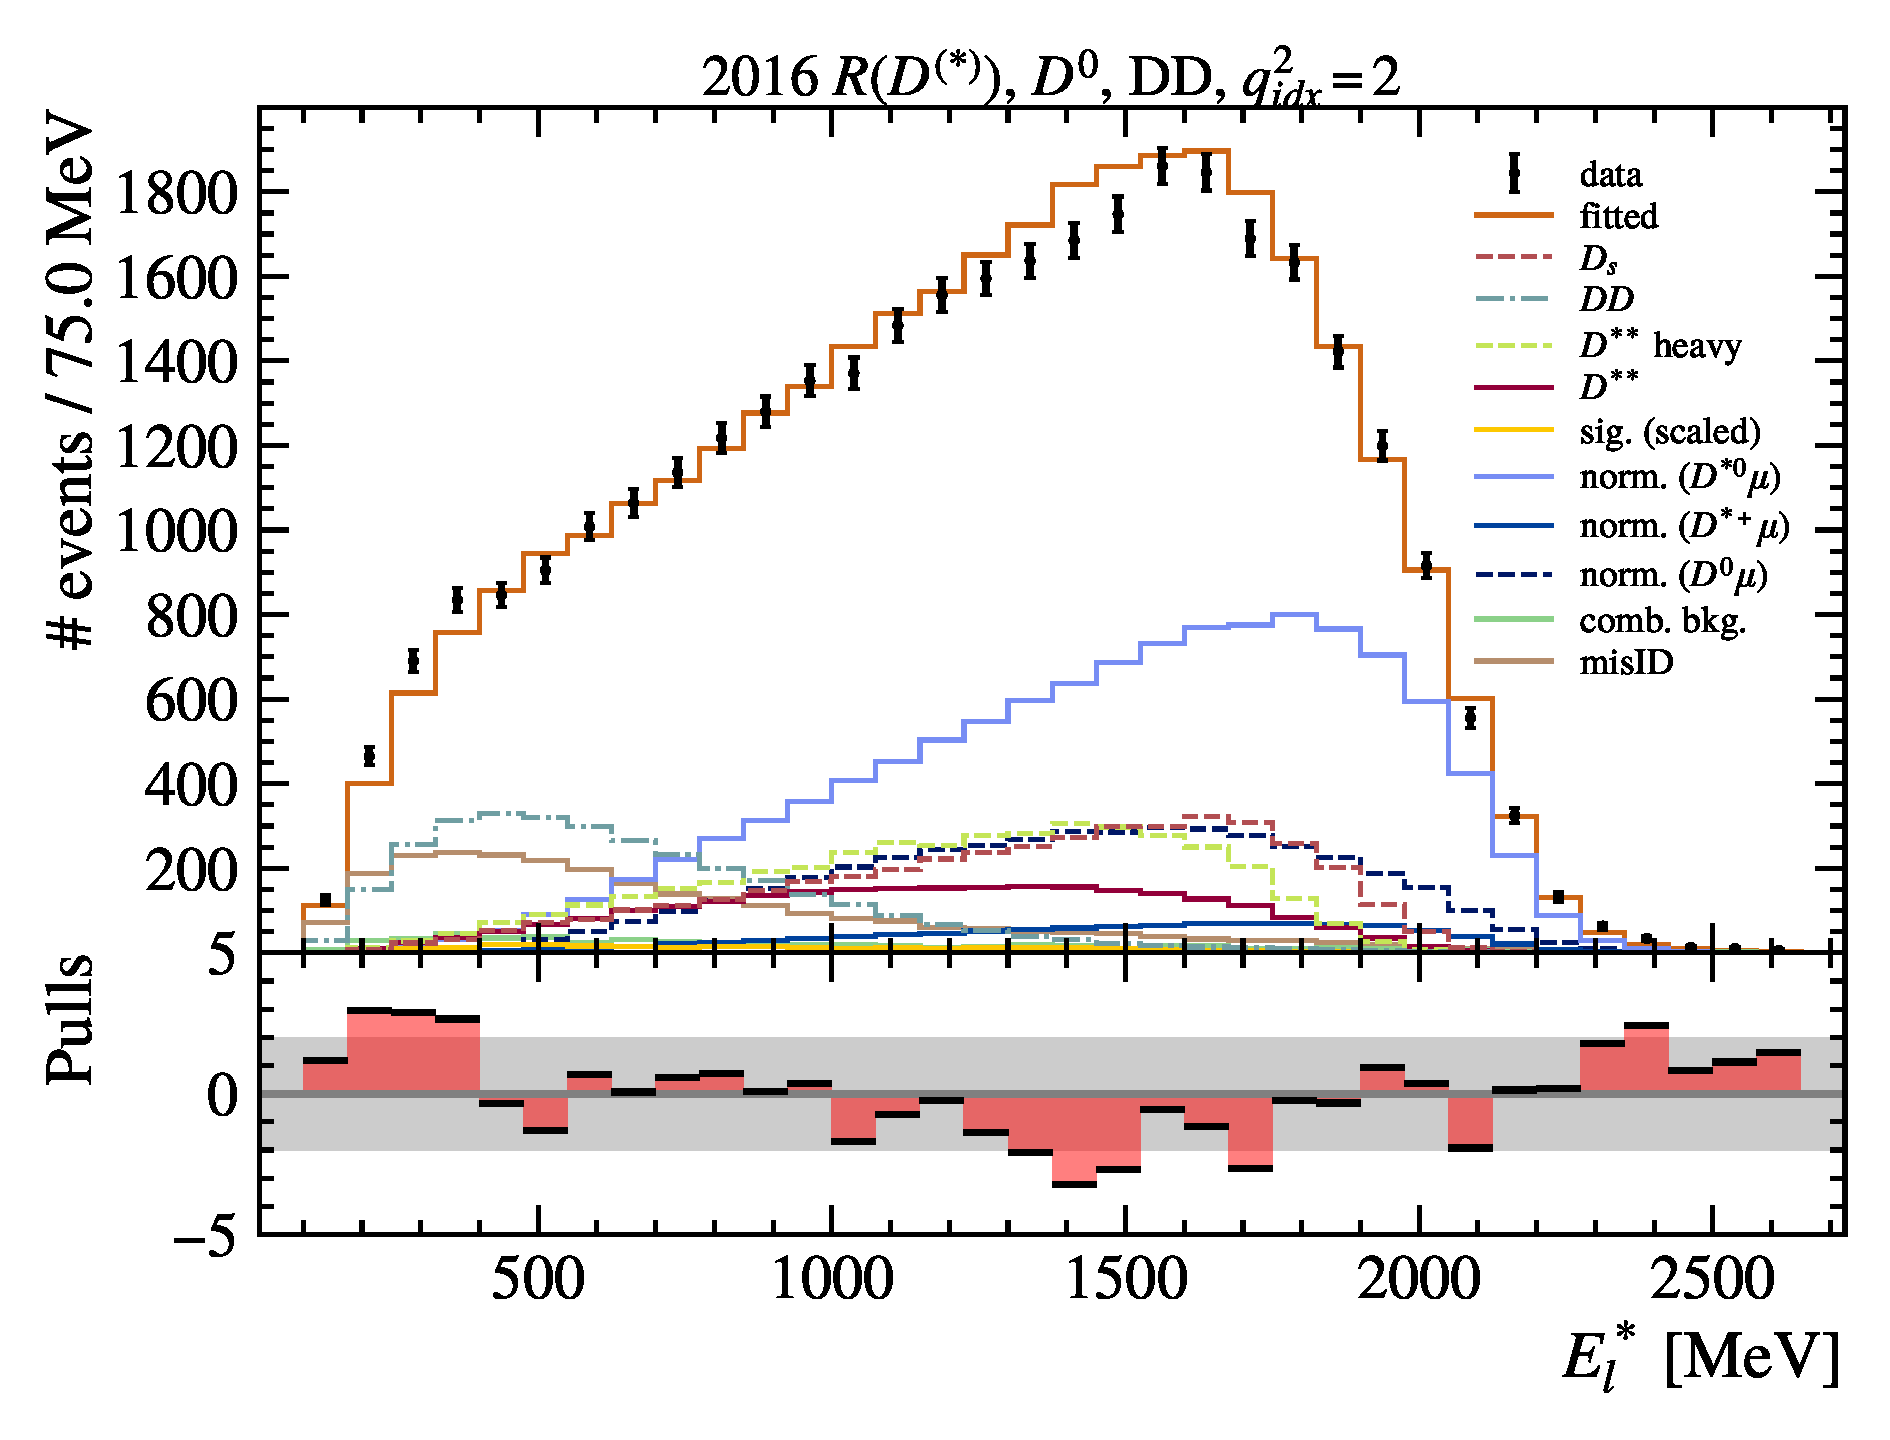
\includegraphics[width=0.24\textwidth]{./figs-fit-to-data/ctrl-fit/lines_q2_slices/fit_result-lines_q2_idx2-D0-dd-el.pdf}
    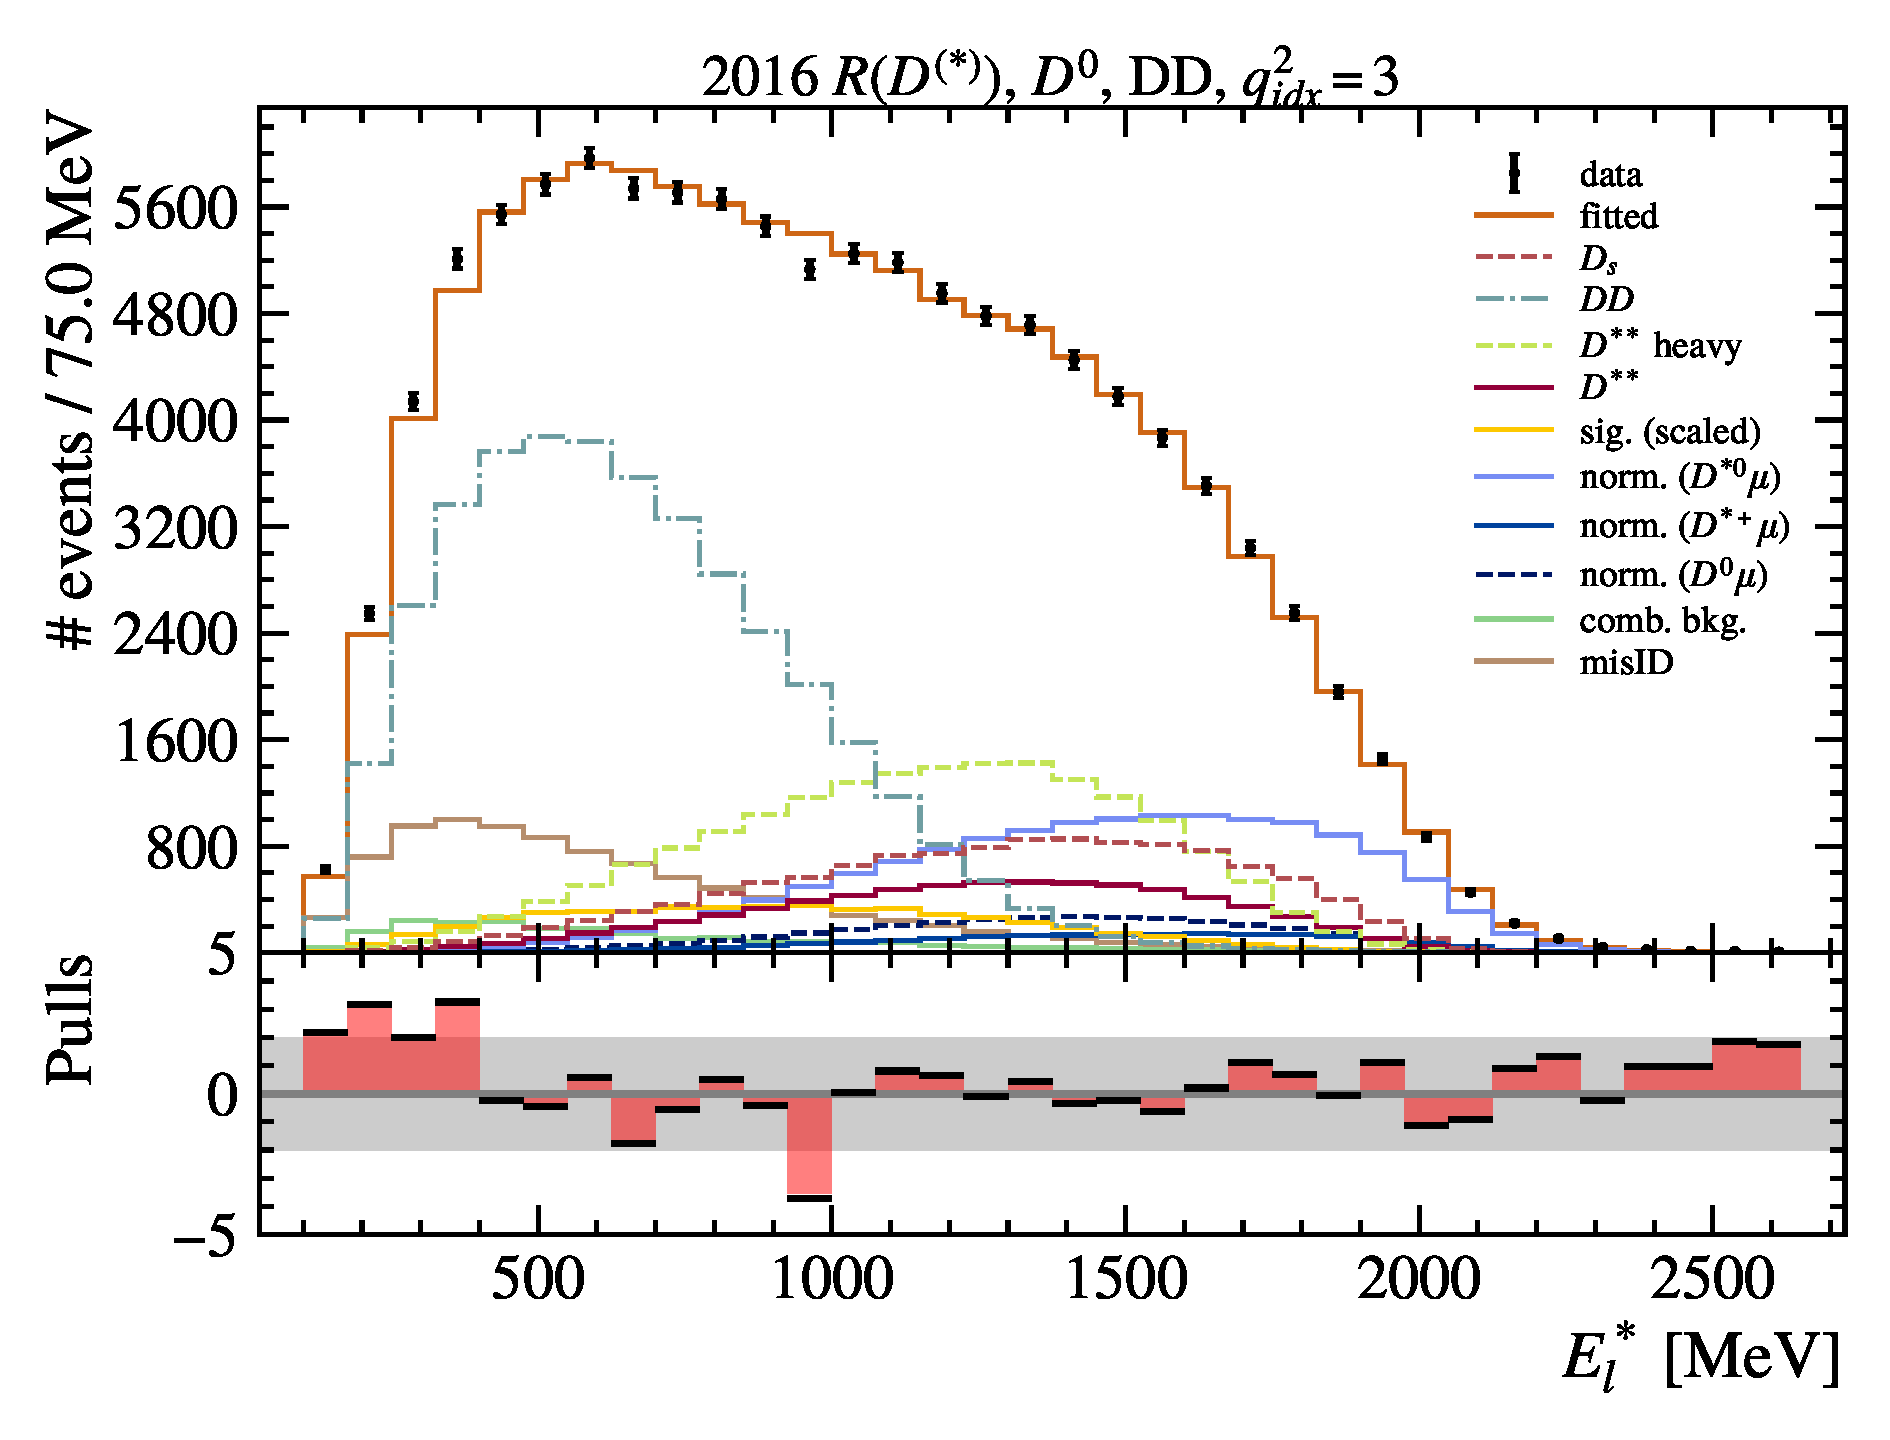
\includegraphics[width=0.24\textwidth]{./figs-fit-to-data/ctrl-fit/lines_q2_slices/fit_result-lines_q2_idx3-D0-dd-el.pdf}
    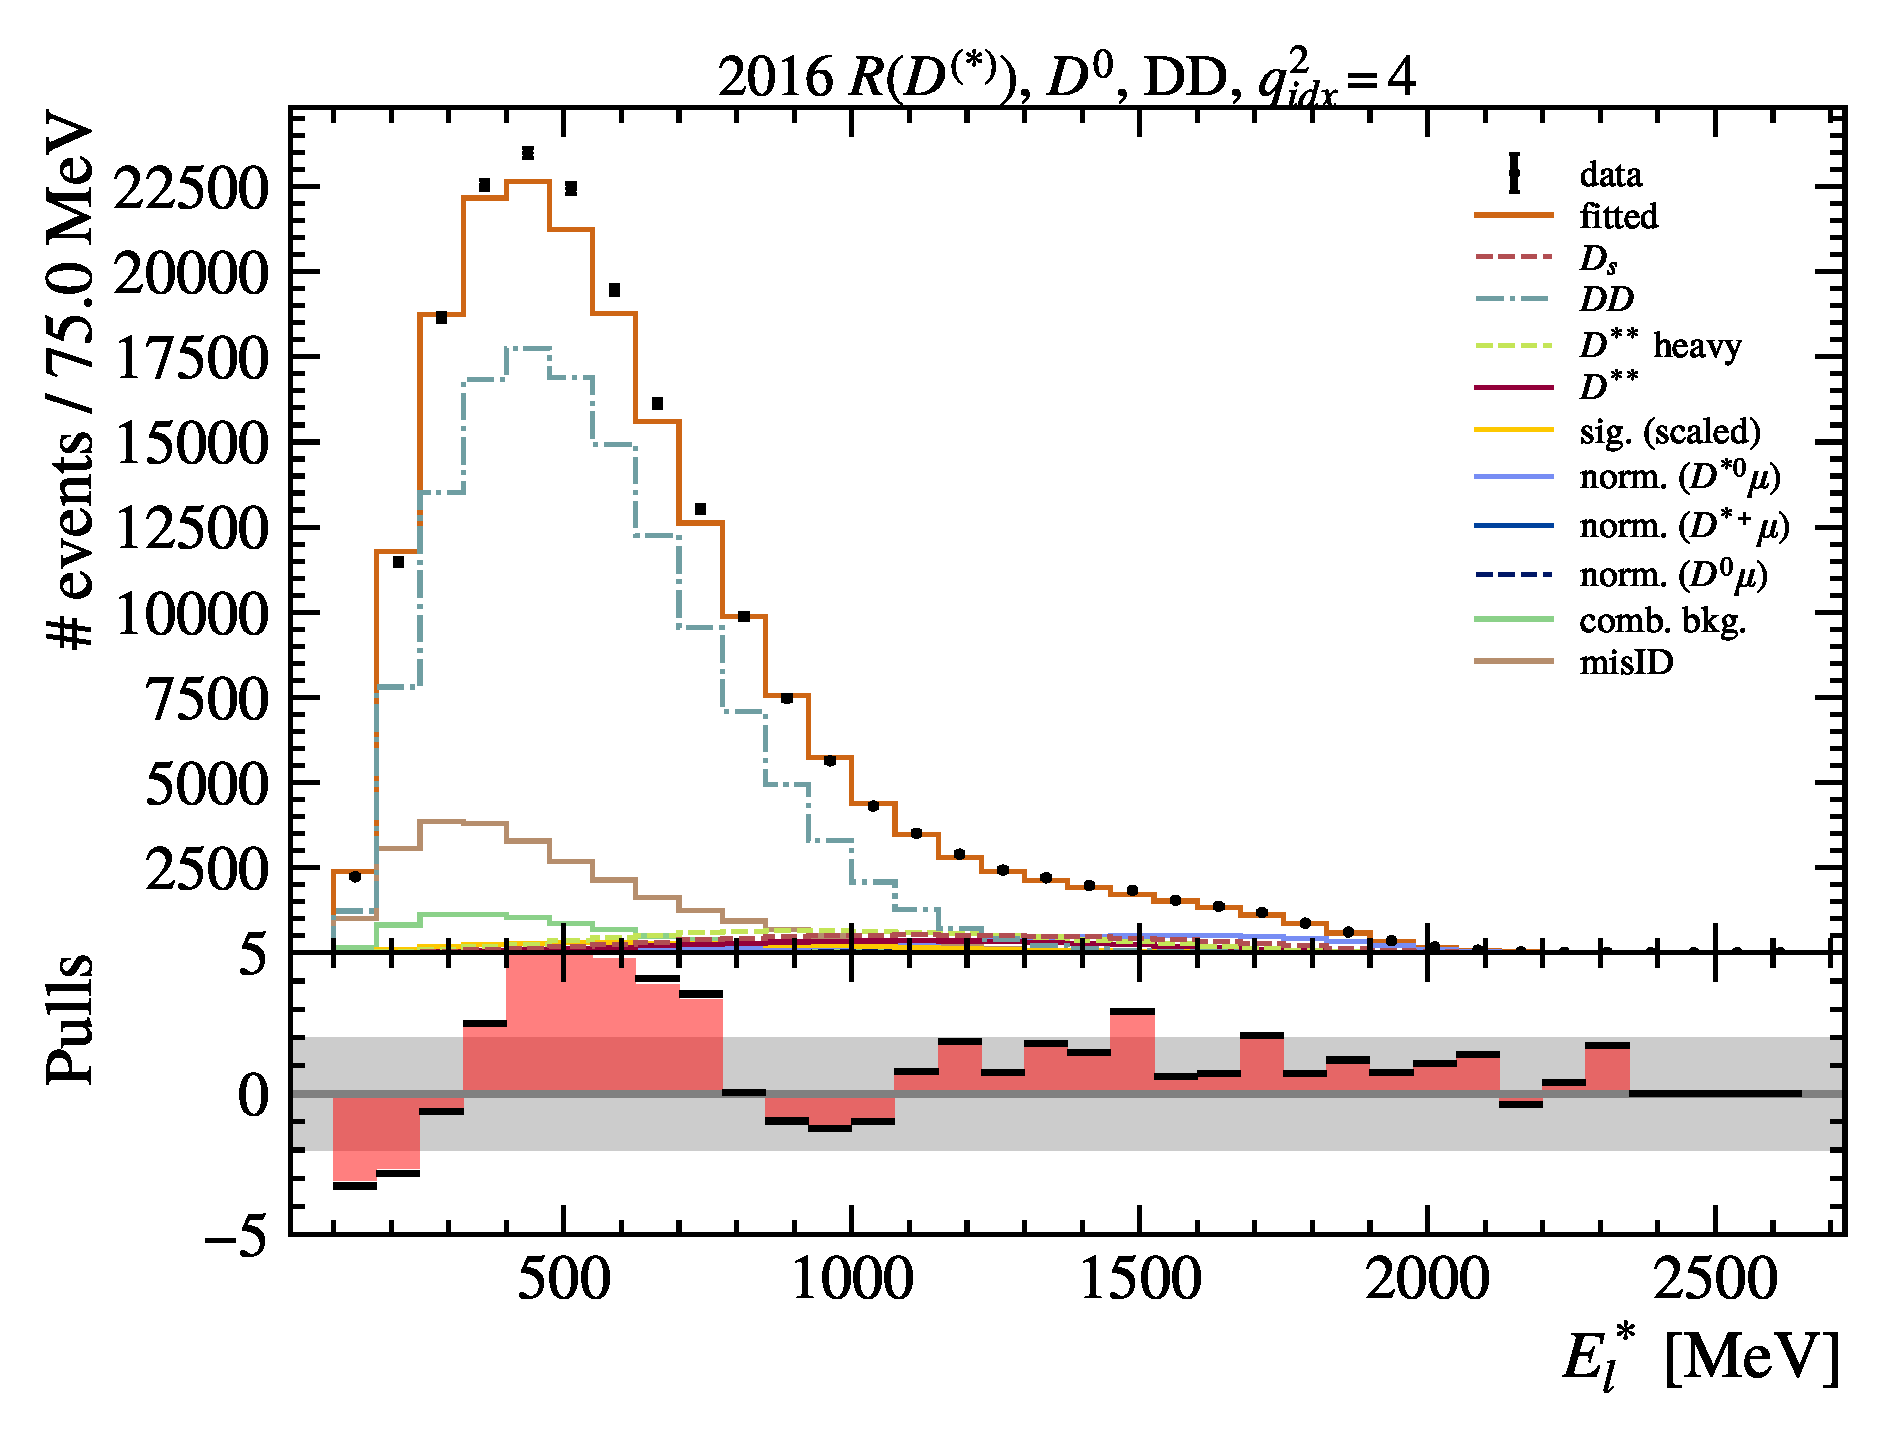
\includegraphics[width=0.24\textwidth]{./figs-fit-to-data/ctrl-fit/lines_q2_slices/fit_result-lines_q2_idx4-D0-dd-el.pdf}

    \caption{Control fit for DD sample, \Dz channel.}
    \label{fig:ctrl-dd-d0}
\end{figure}

\begin{figure}[htb]
    \centering
    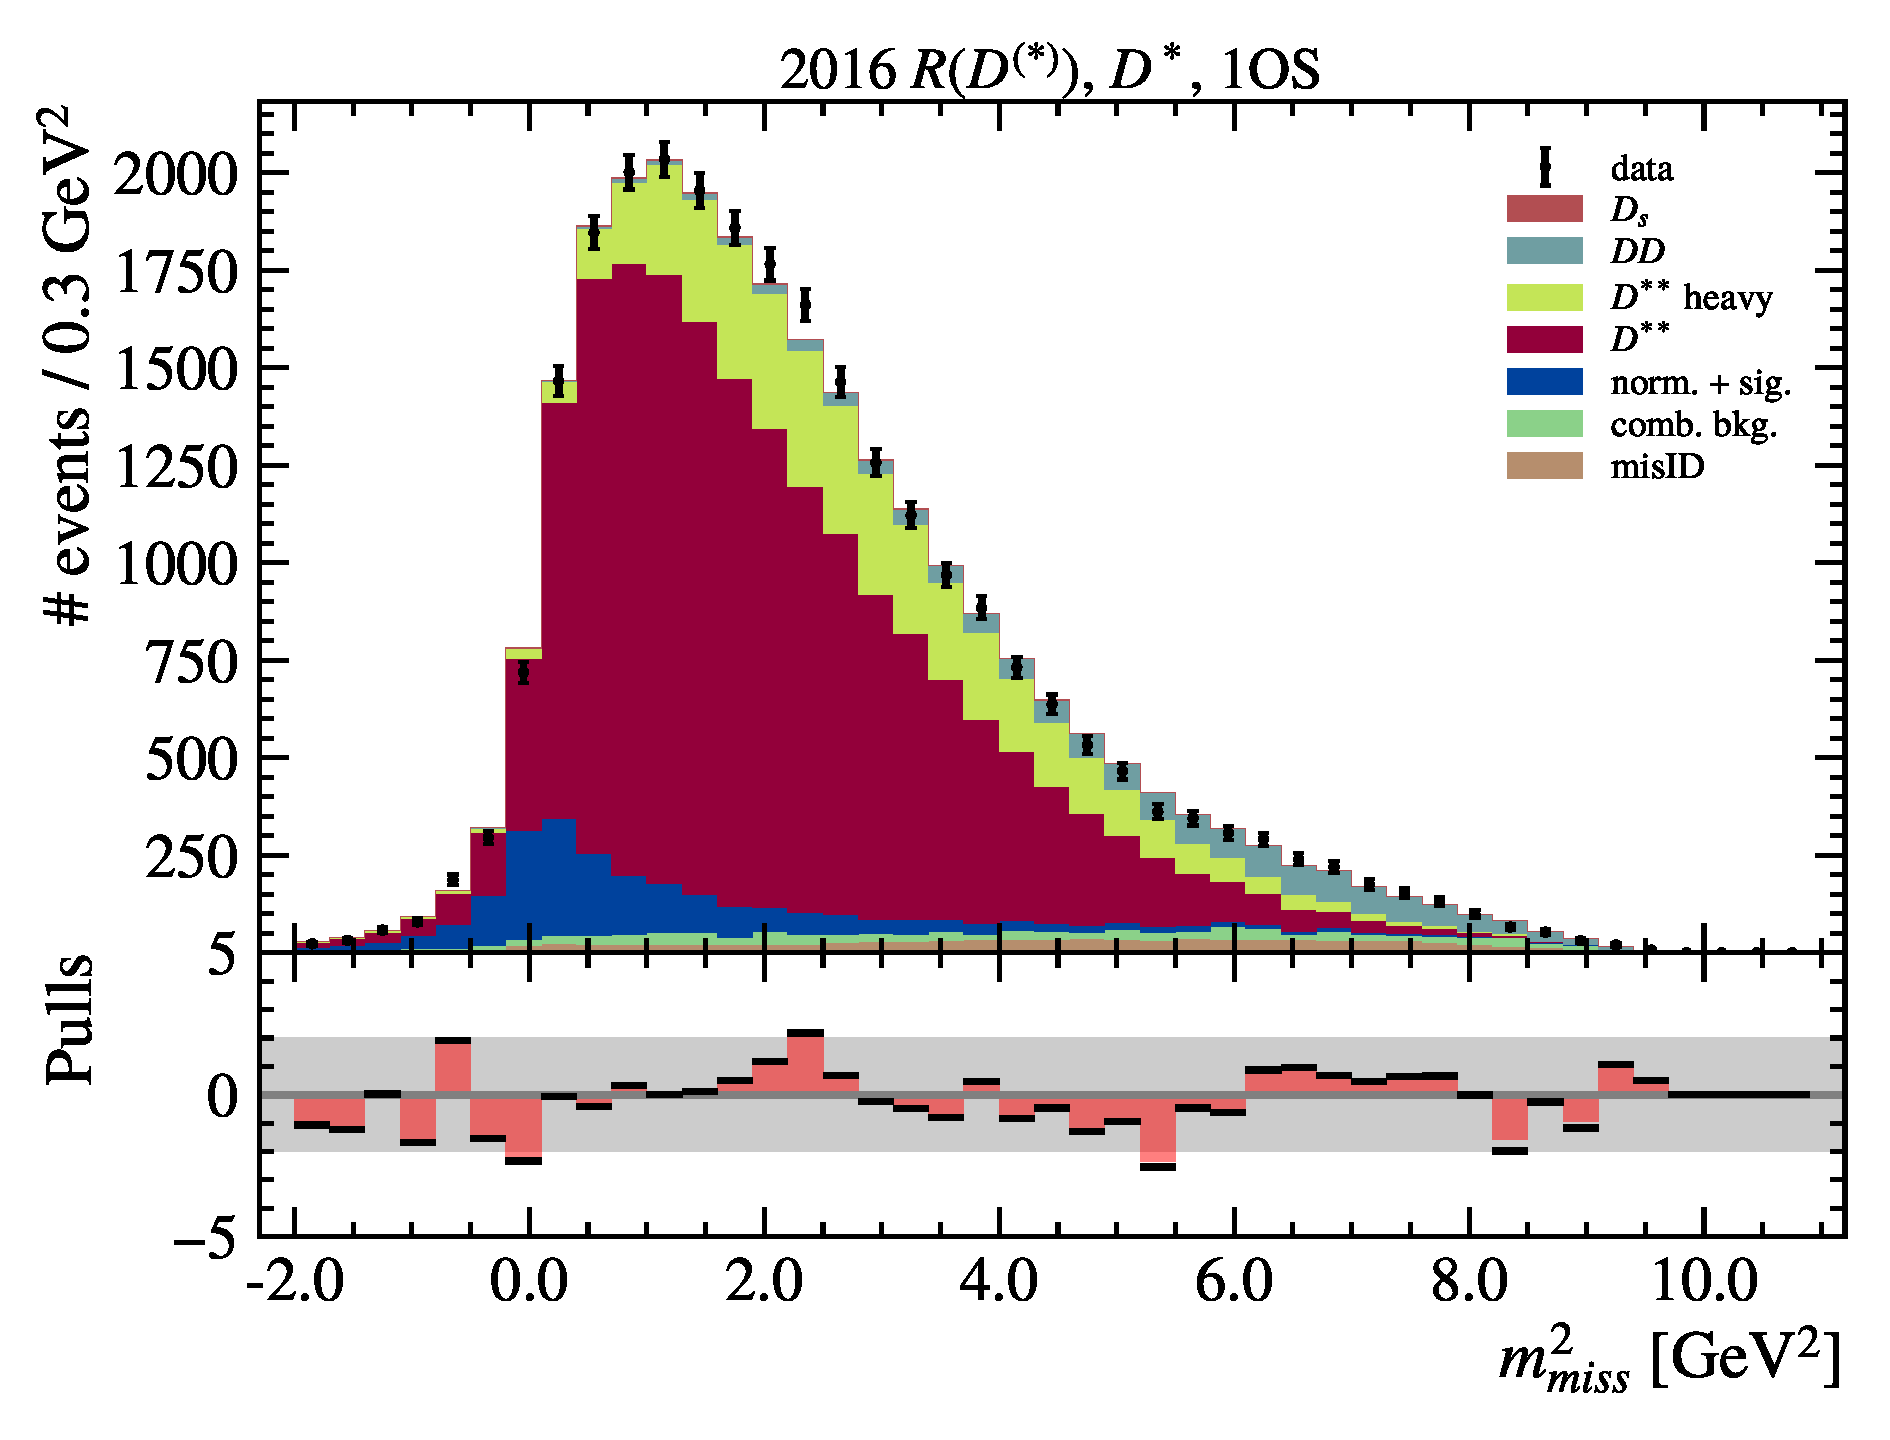
\includegraphics[width=0.32\textwidth]{./figs-fit-to-data/ctrl-fit/stacked/fit_result-stacked-Dst-1os-mmiss2.pdf}
    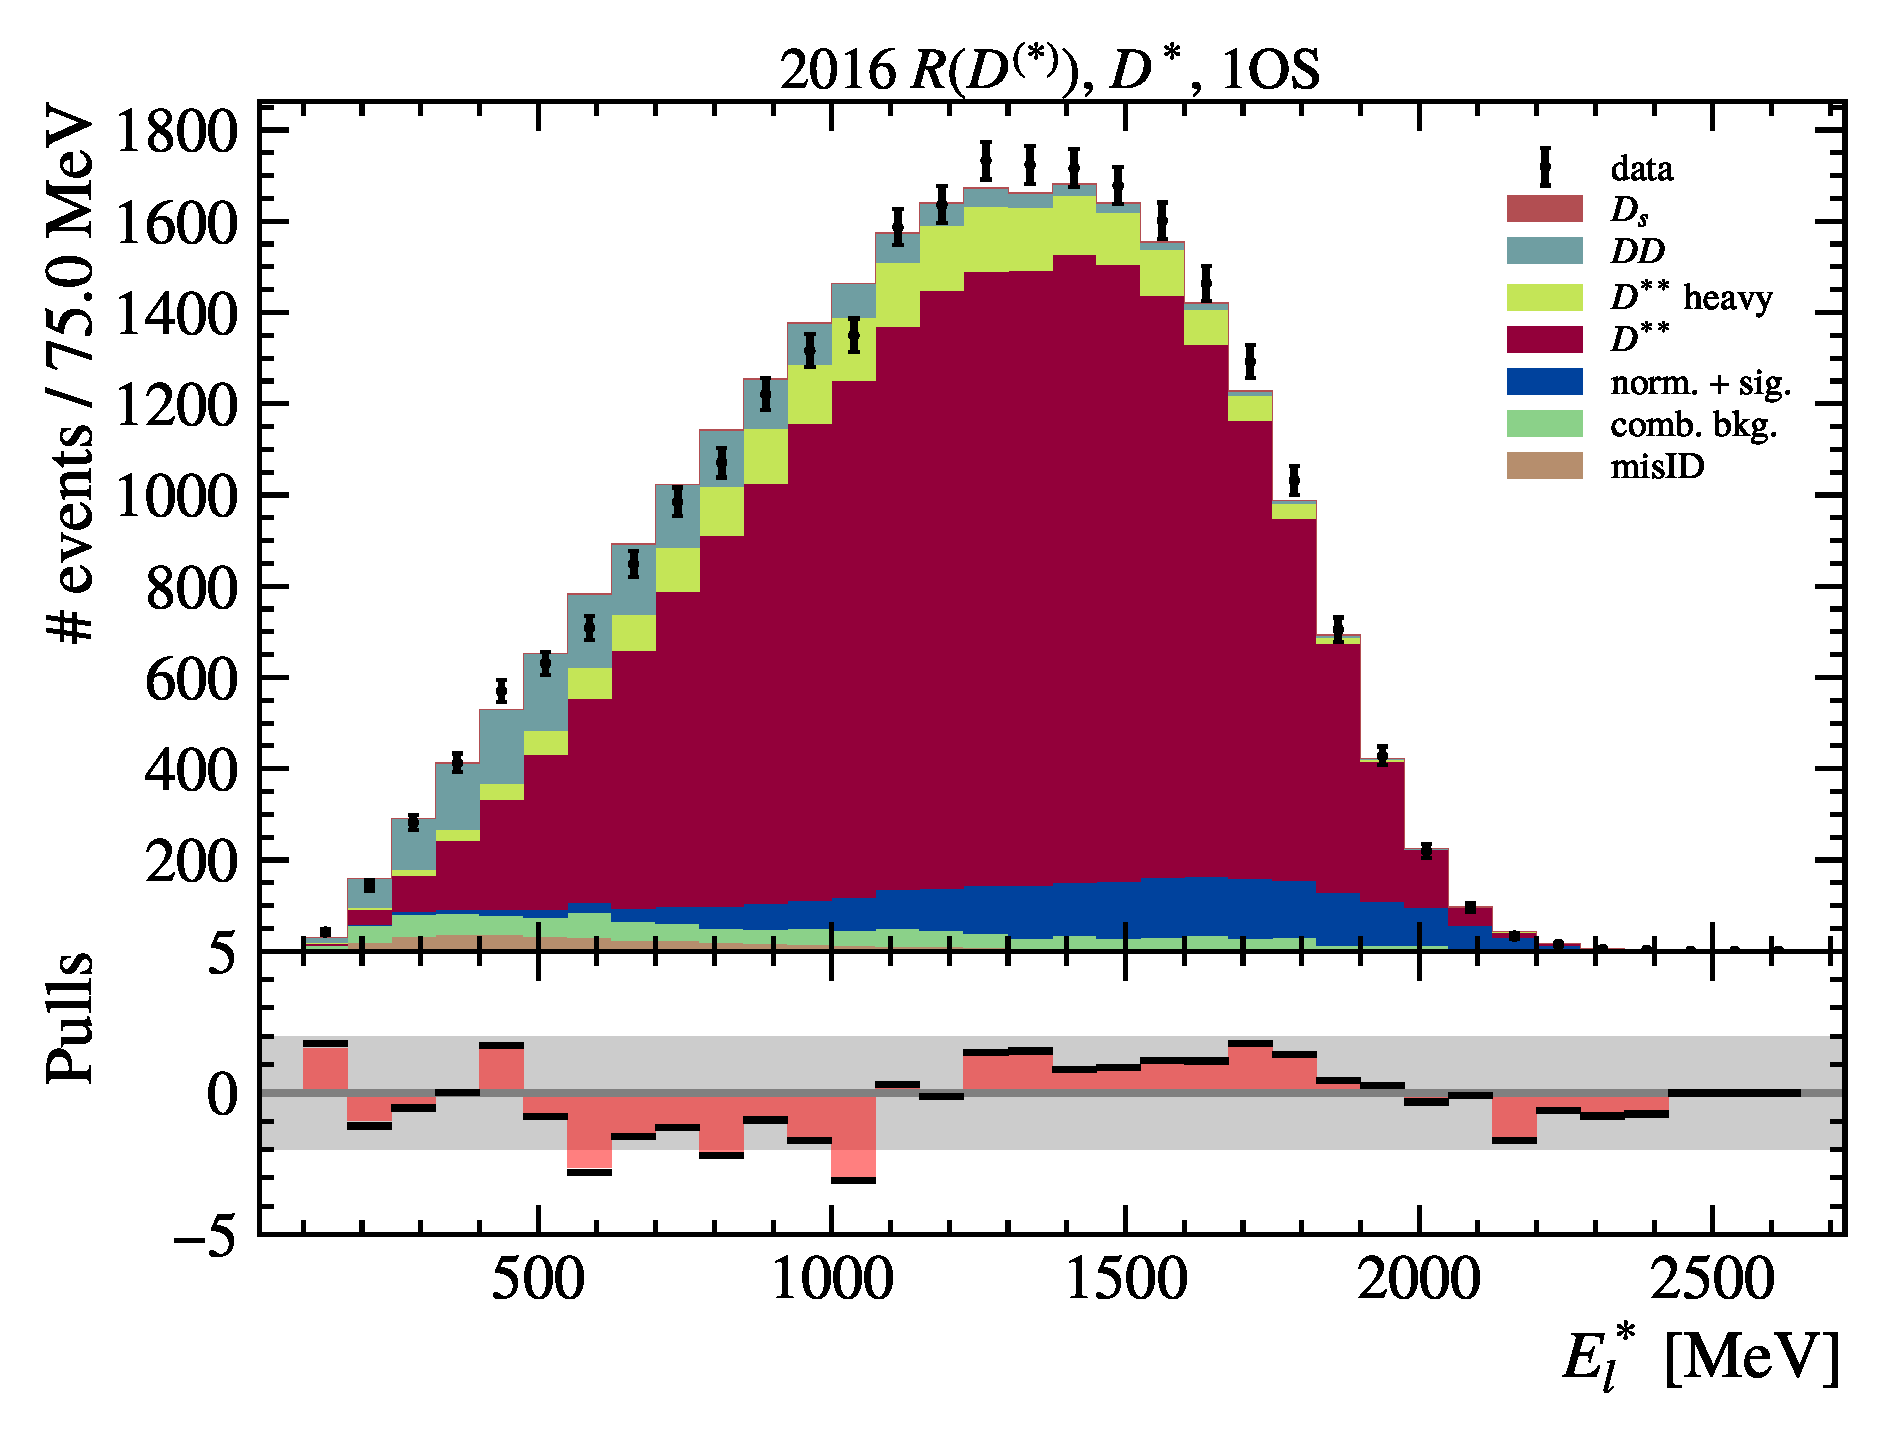
\includegraphics[width=0.32\textwidth]{./figs-fit-to-data/ctrl-fit/stacked/fit_result-stacked-Dst-1os-el.pdf}
    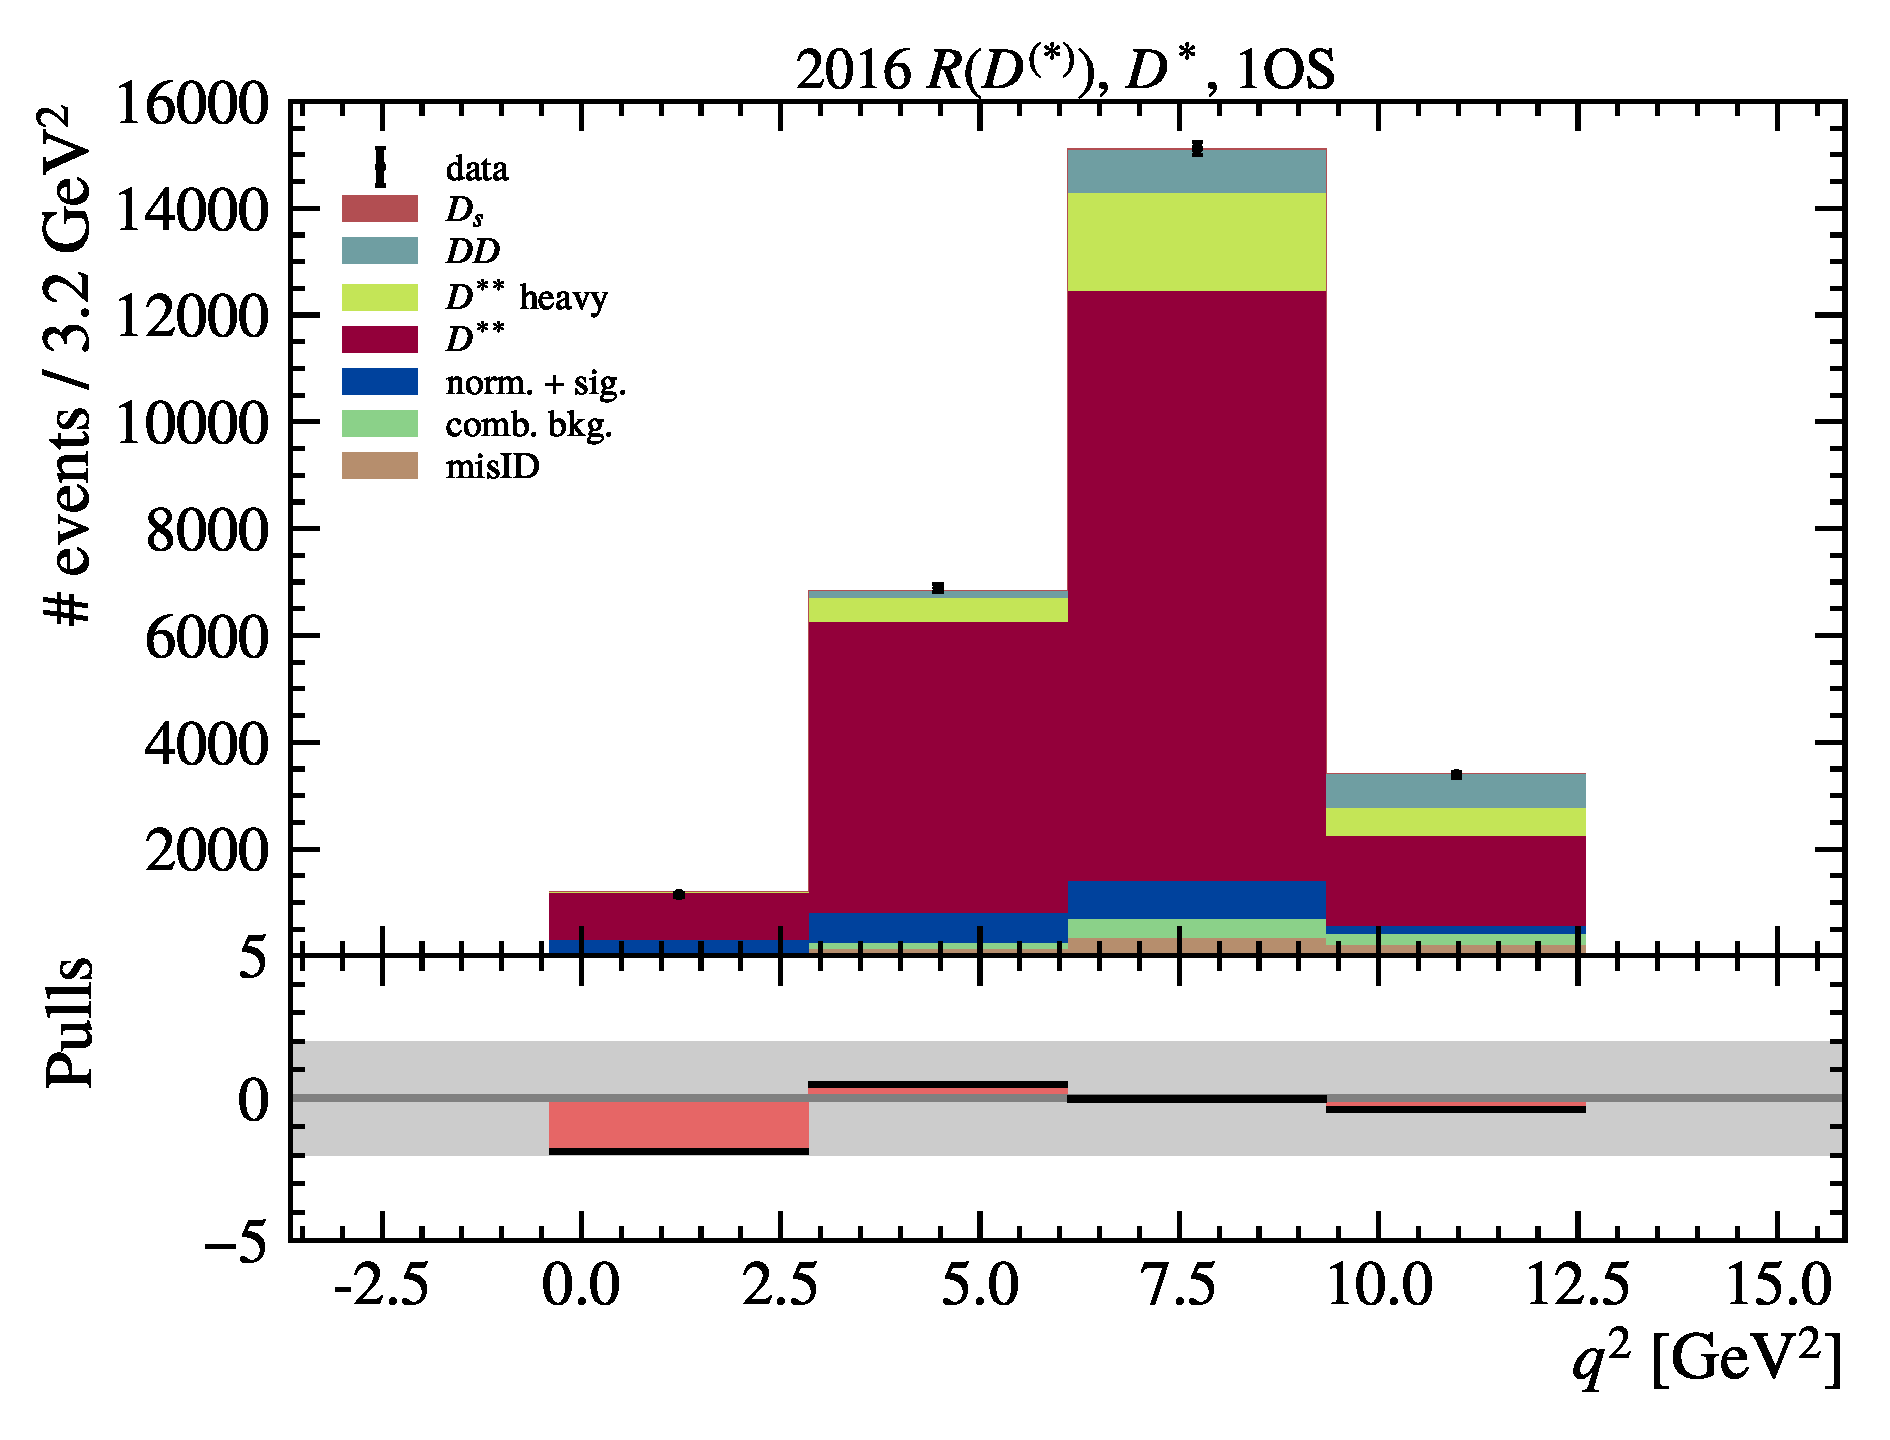
\includegraphics[width=0.32\textwidth]{./figs-fit-to-data/ctrl-fit/stacked/fit_result-stacked-Dst-1os-q2.pdf}

    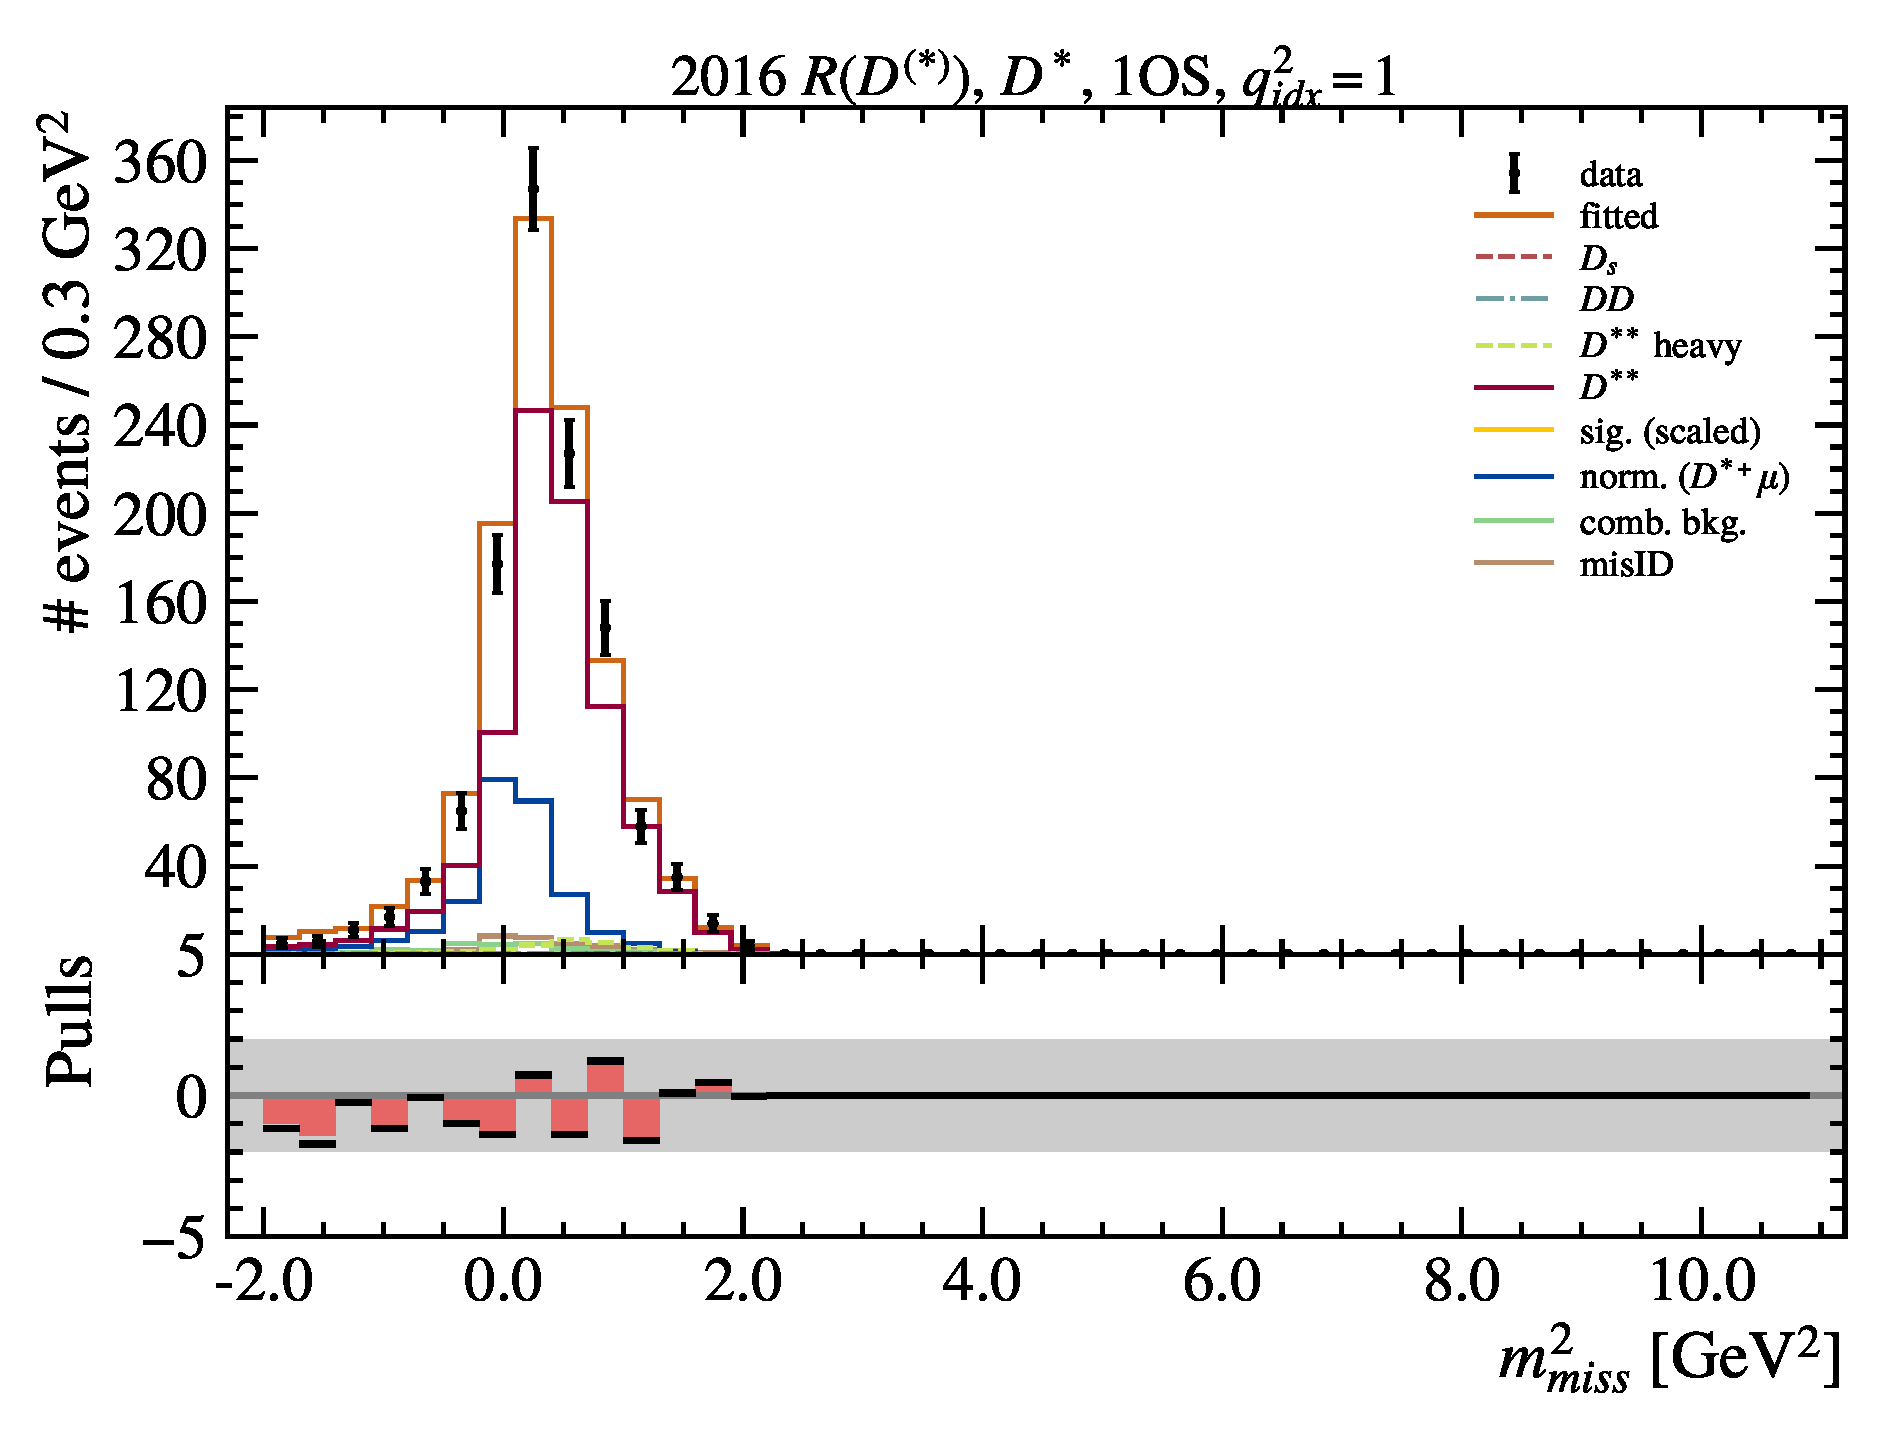
\includegraphics[width=0.24\textwidth]{./figs-fit-to-data/ctrl-fit/lines_q2_slices/fit_result-lines_q2_idx1-Dst-1os-mmiss2.pdf}
    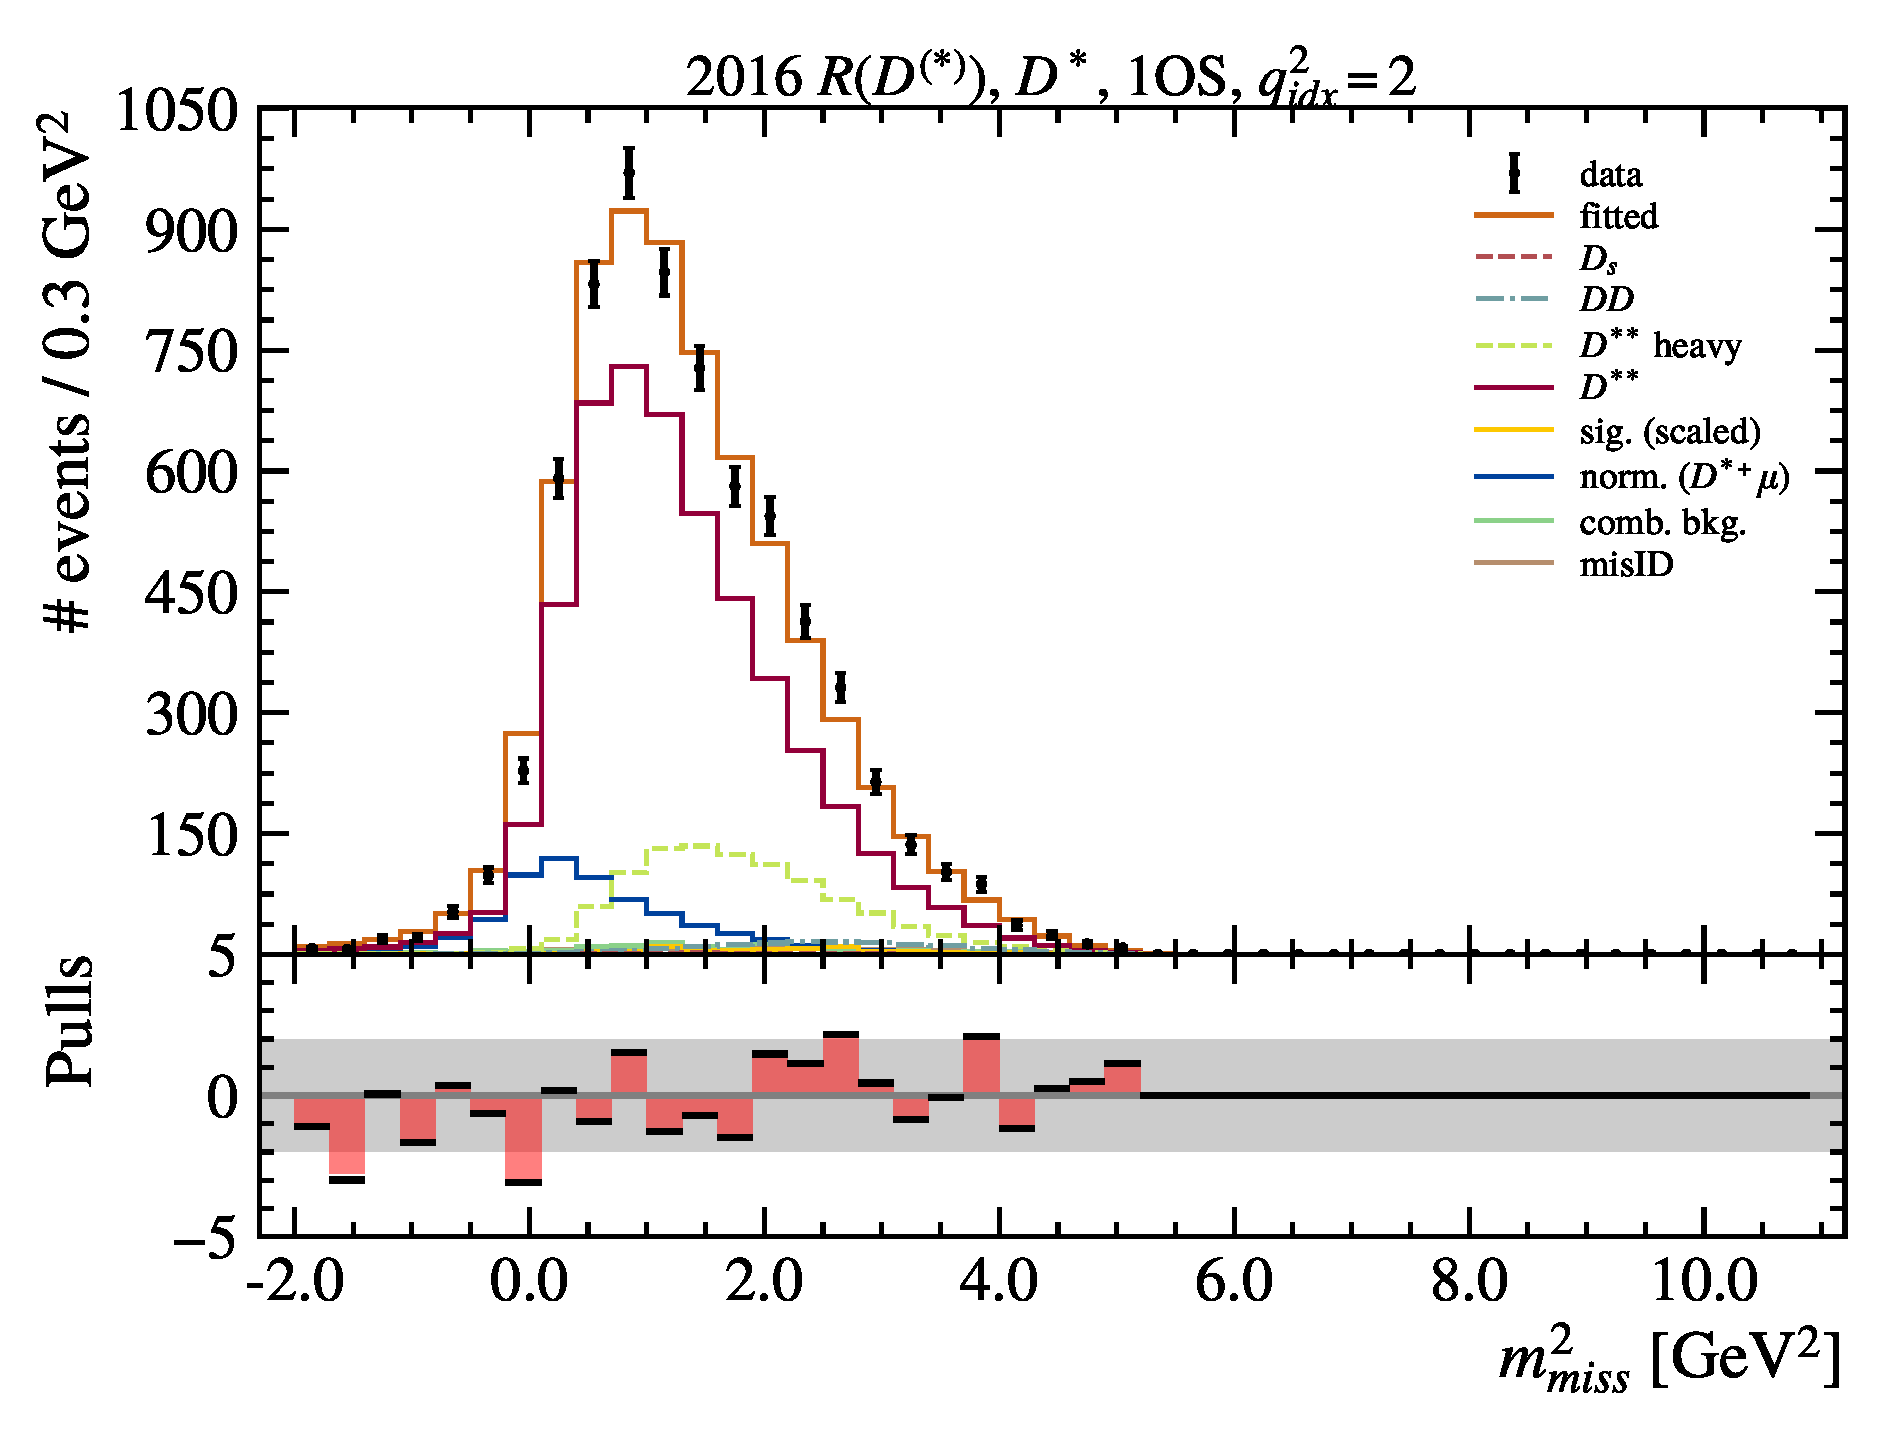
\includegraphics[width=0.24\textwidth]{./figs-fit-to-data/ctrl-fit/lines_q2_slices/fit_result-lines_q2_idx2-Dst-1os-mmiss2.pdf}
    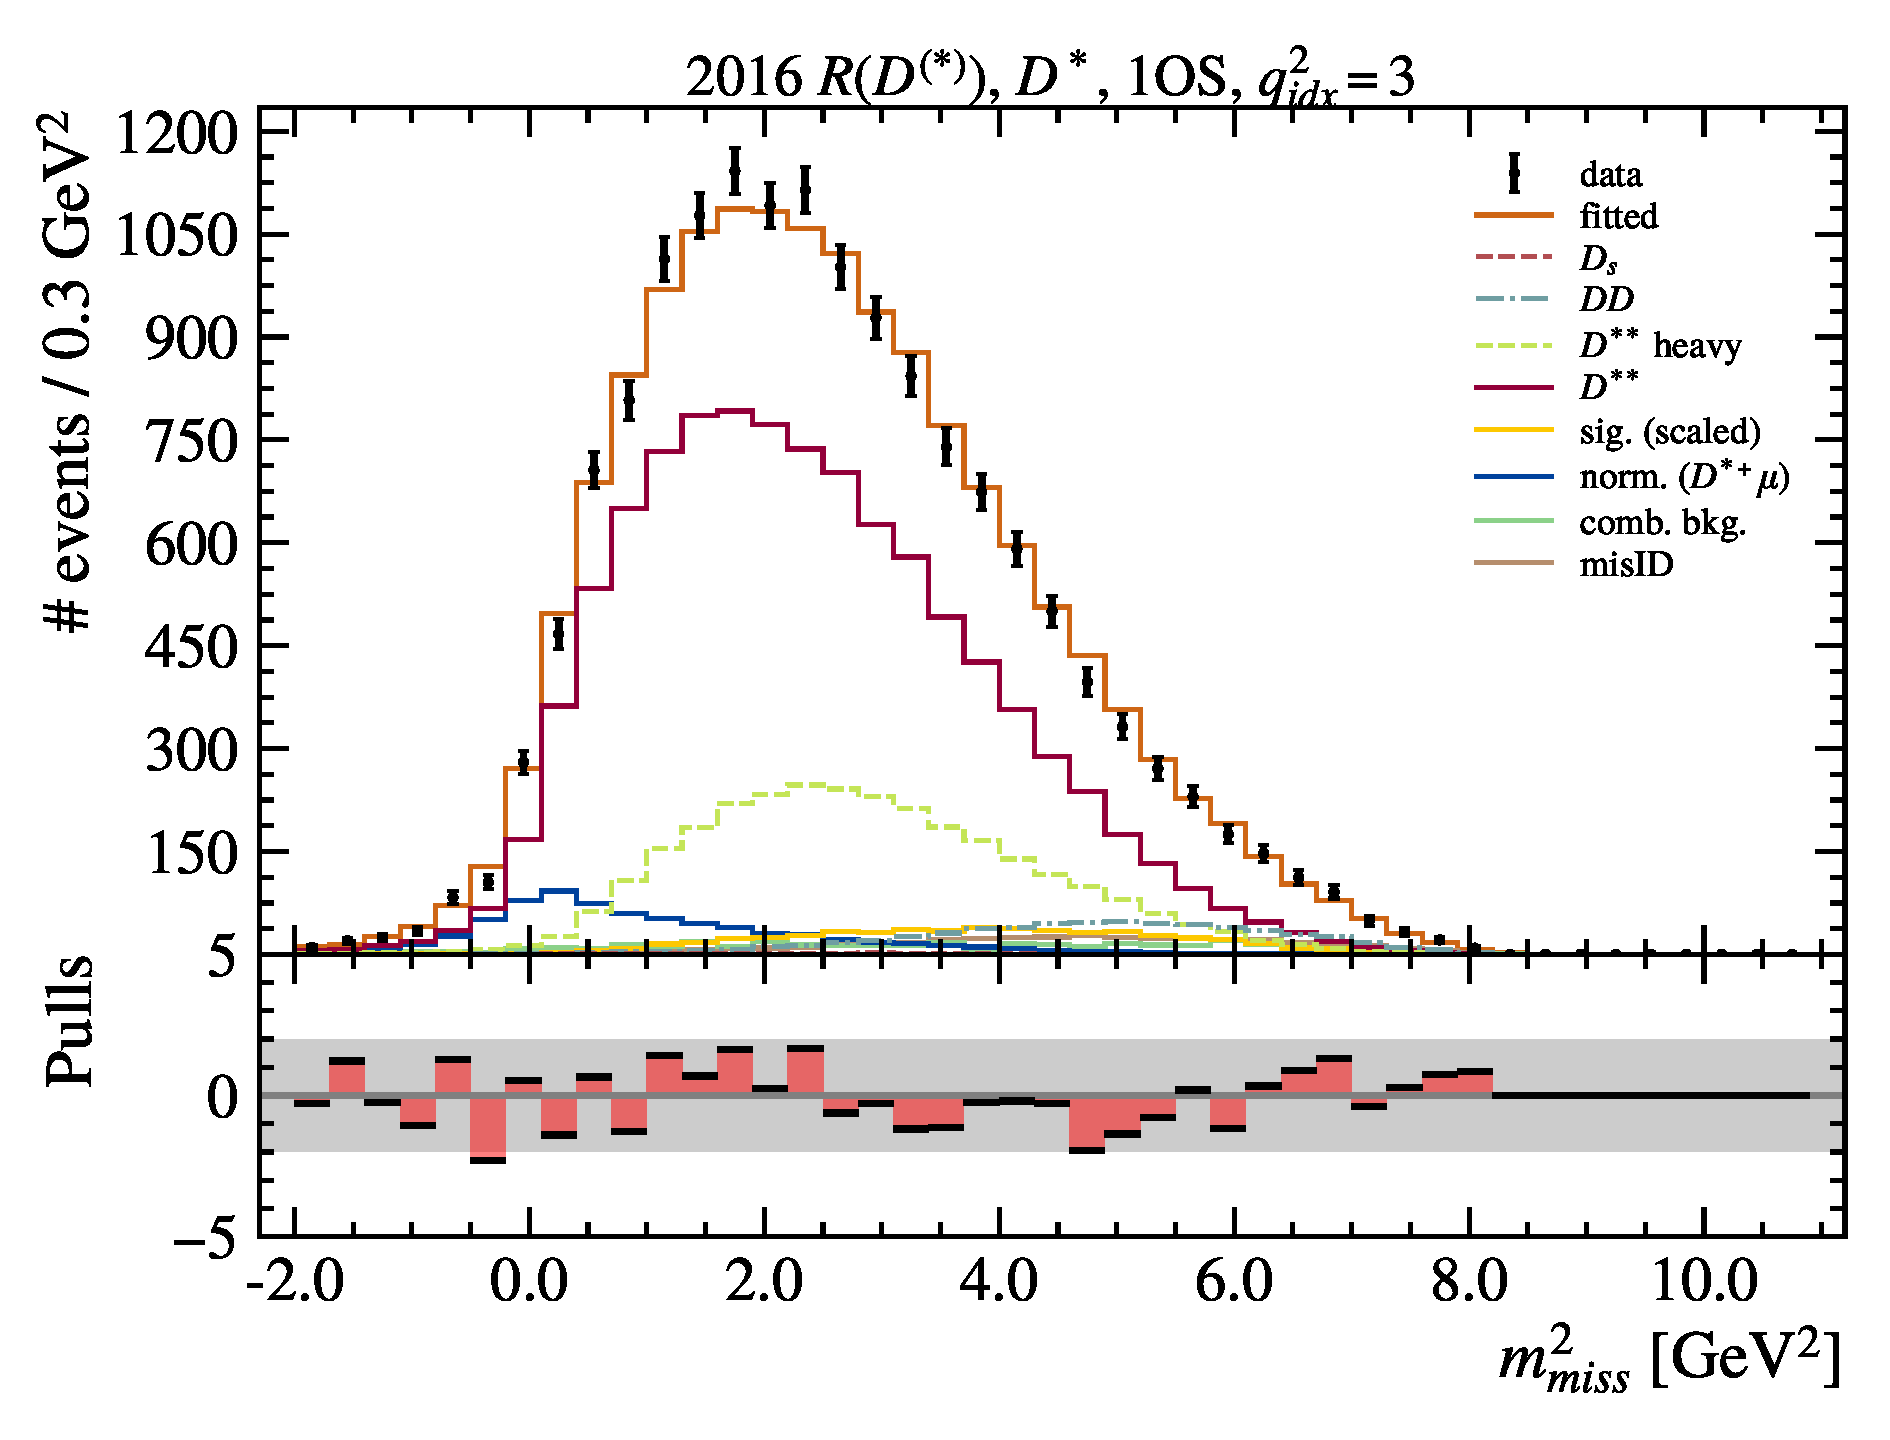
\includegraphics[width=0.24\textwidth]{./figs-fit-to-data/ctrl-fit/lines_q2_slices/fit_result-lines_q2_idx3-Dst-1os-mmiss2.pdf}
    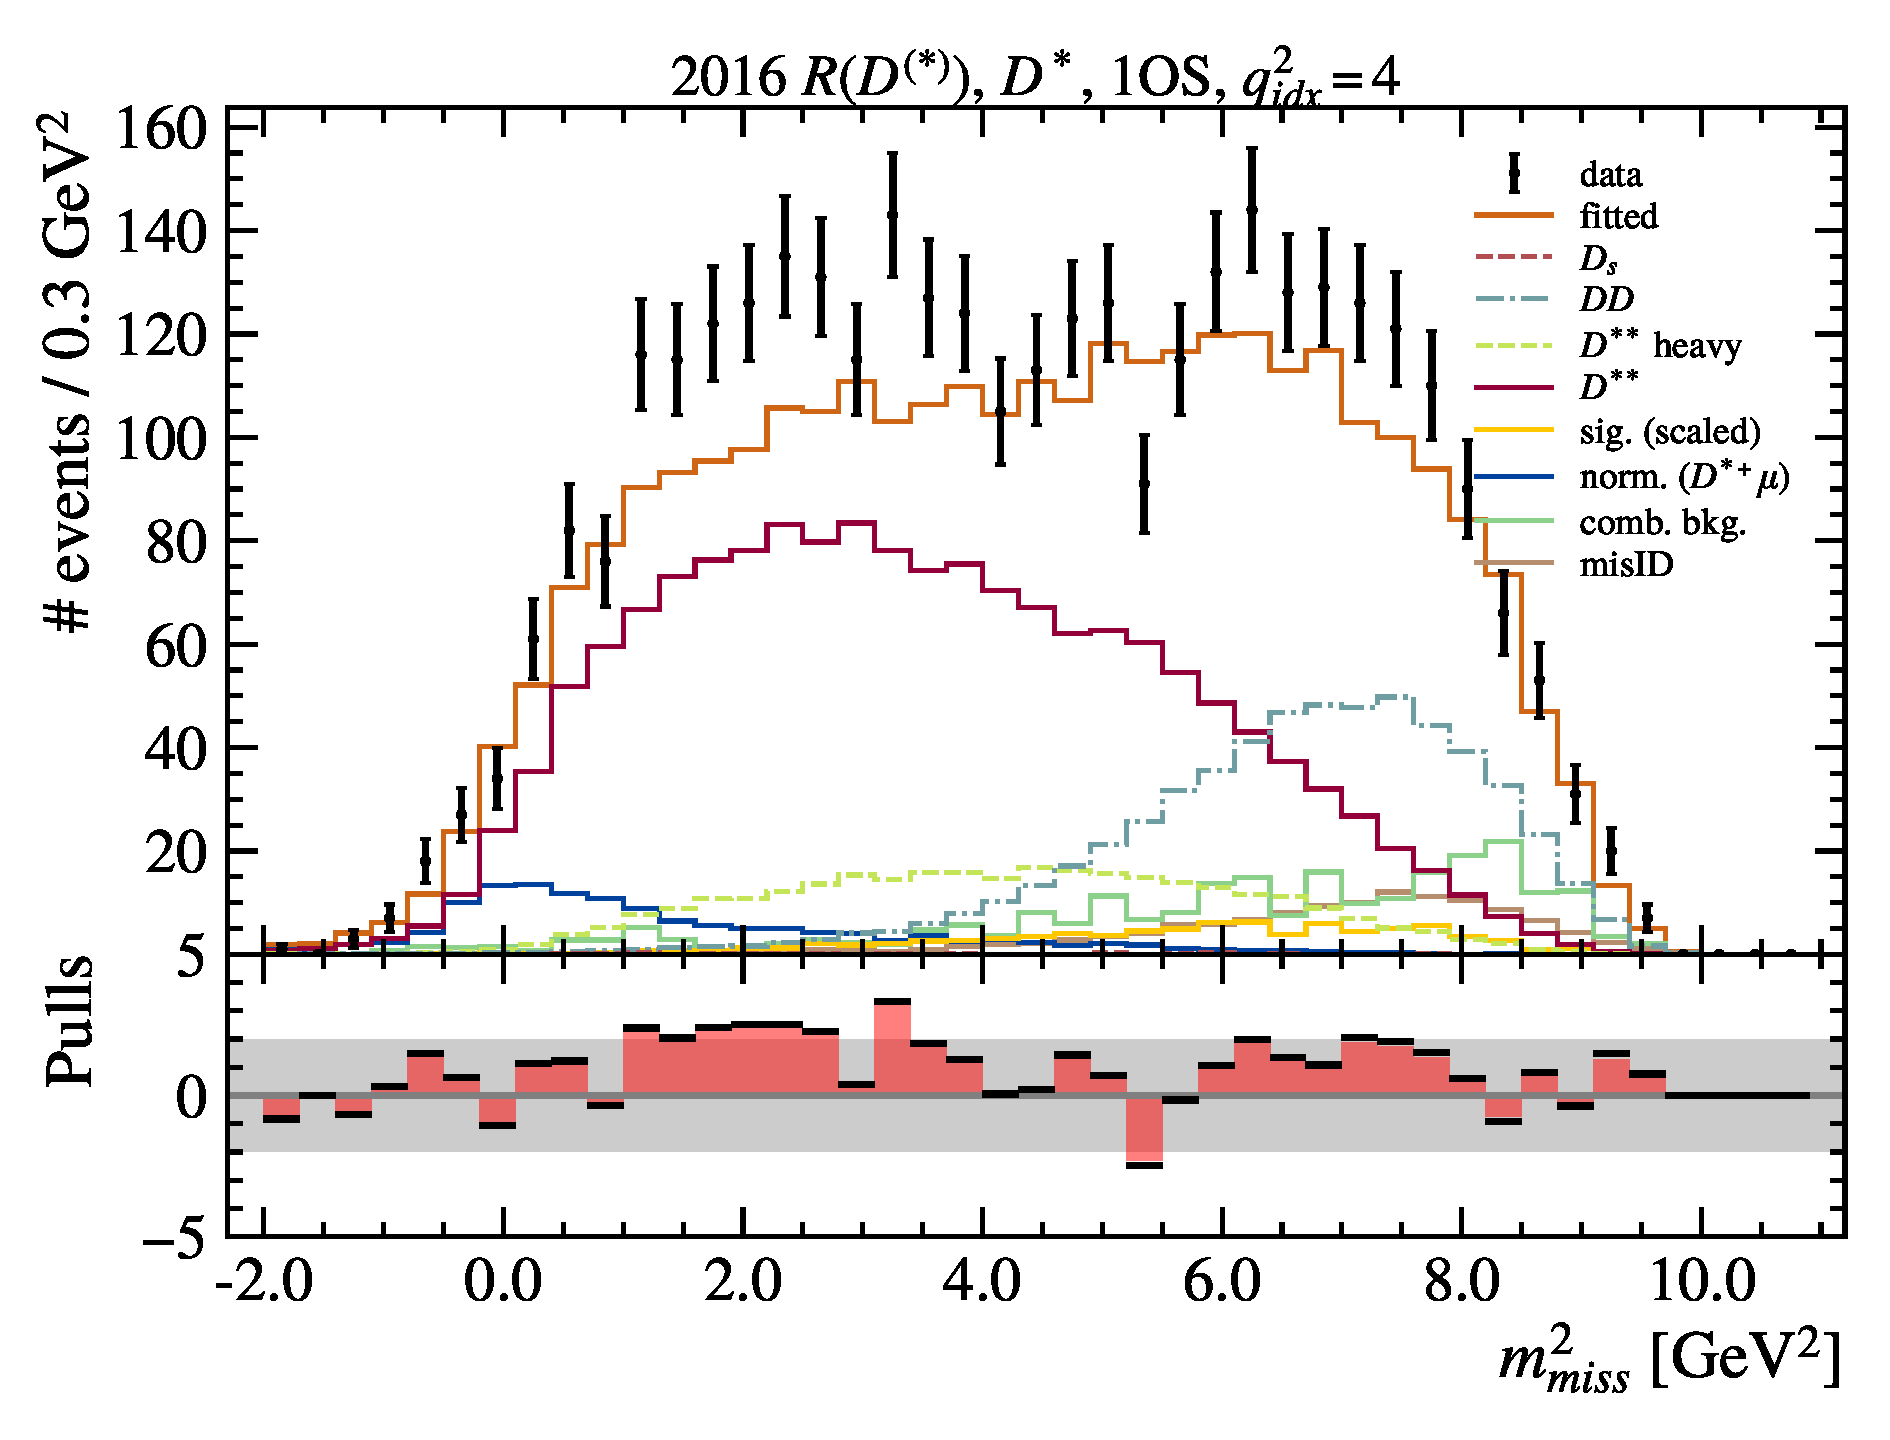
\includegraphics[width=0.24\textwidth]{./figs-fit-to-data/ctrl-fit/lines_q2_slices/fit_result-lines_q2_idx4-Dst-1os-mmiss2.pdf}

    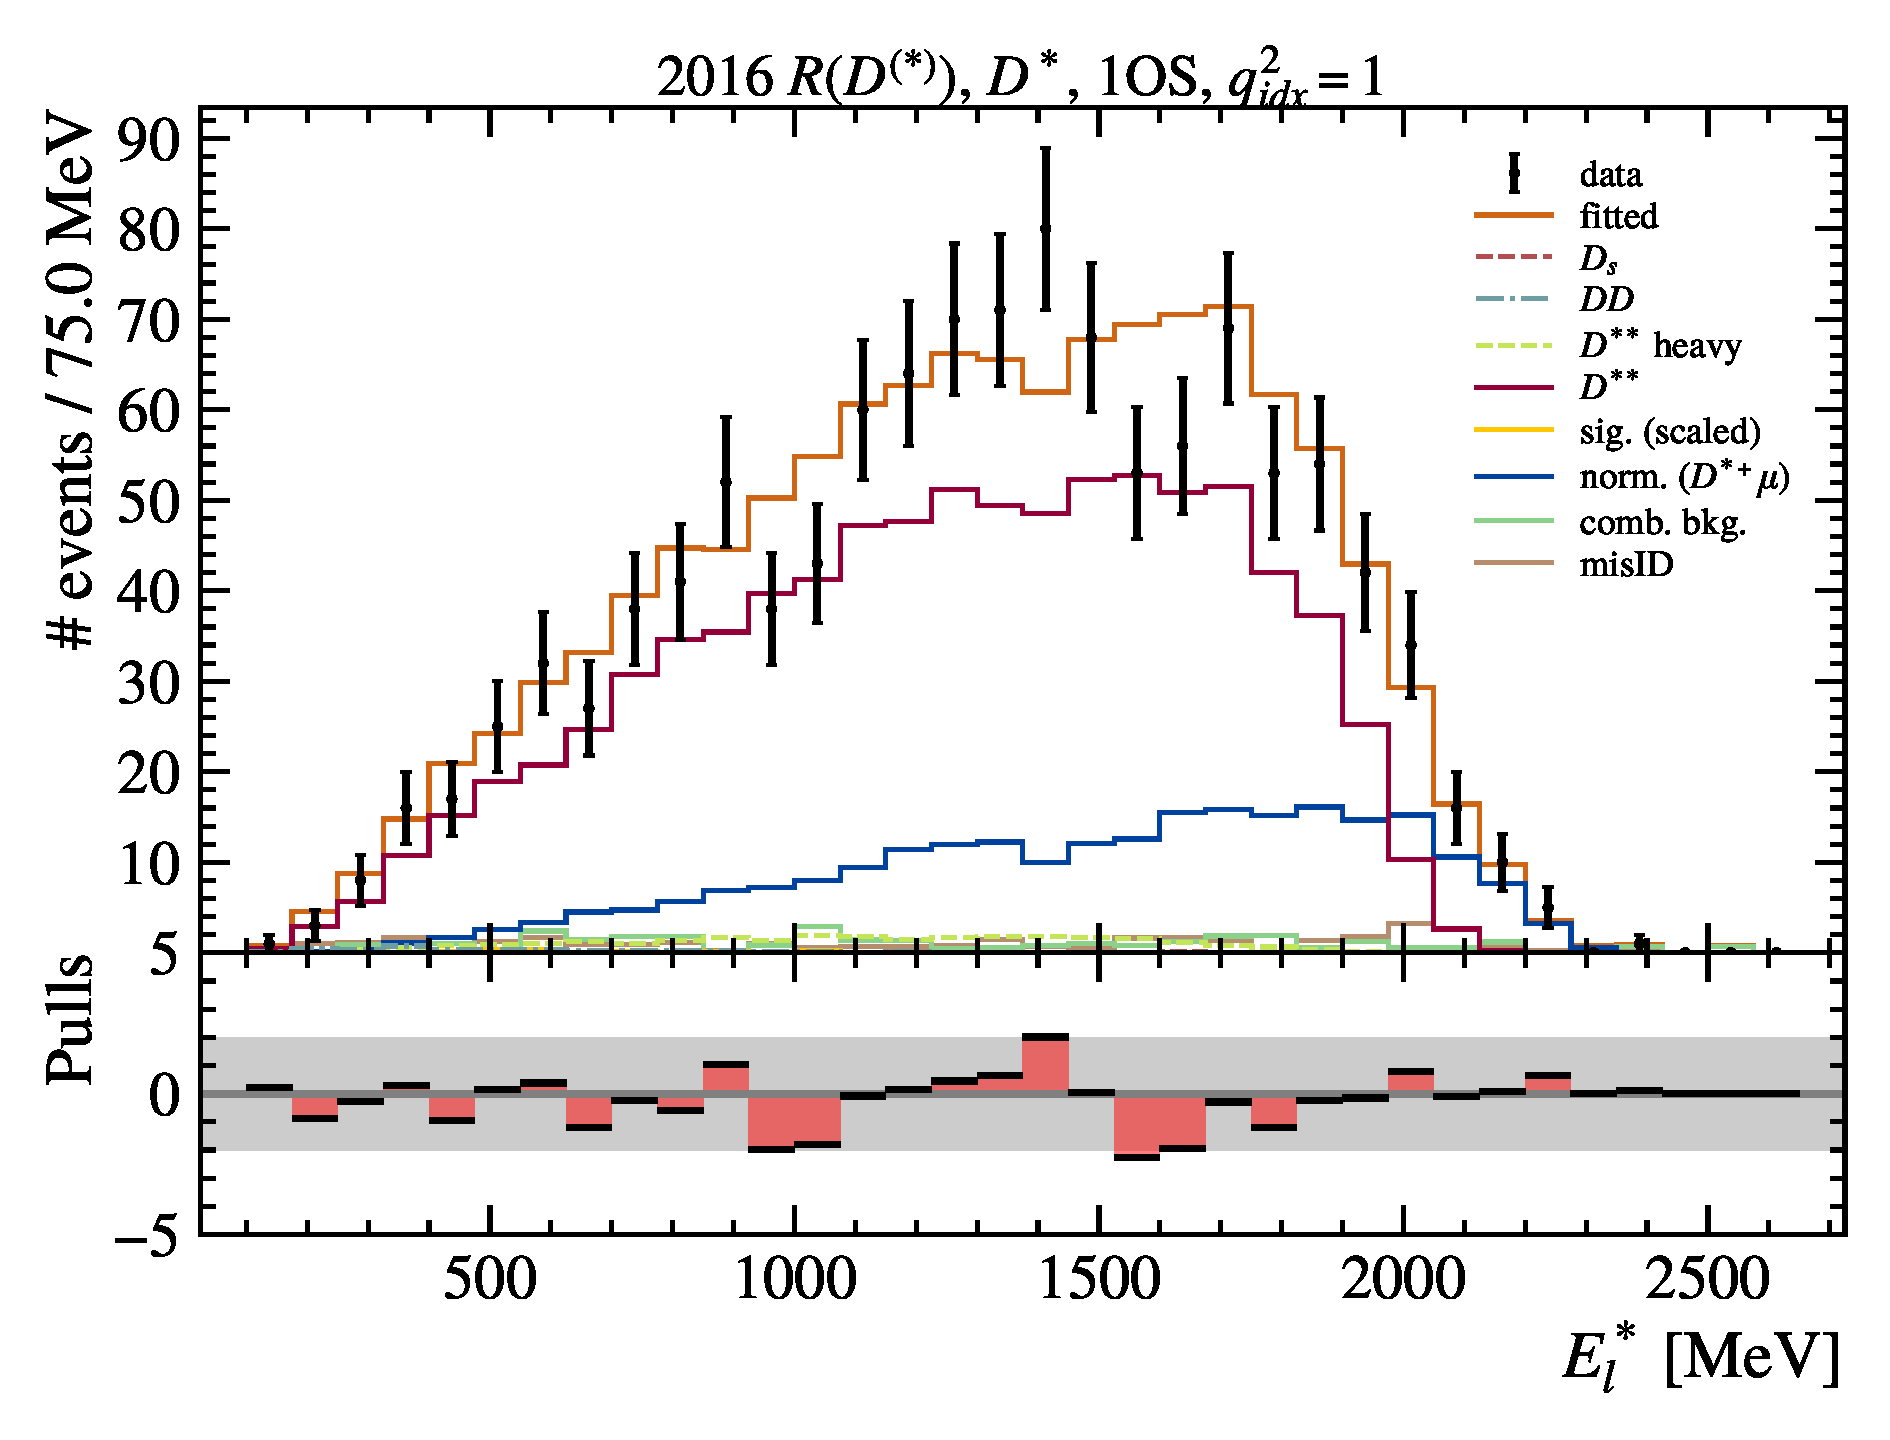
\includegraphics[width=0.24\textwidth]{./figs-fit-to-data/ctrl-fit/lines_q2_slices/fit_result-lines_q2_idx1-Dst-1os-el.pdf}
    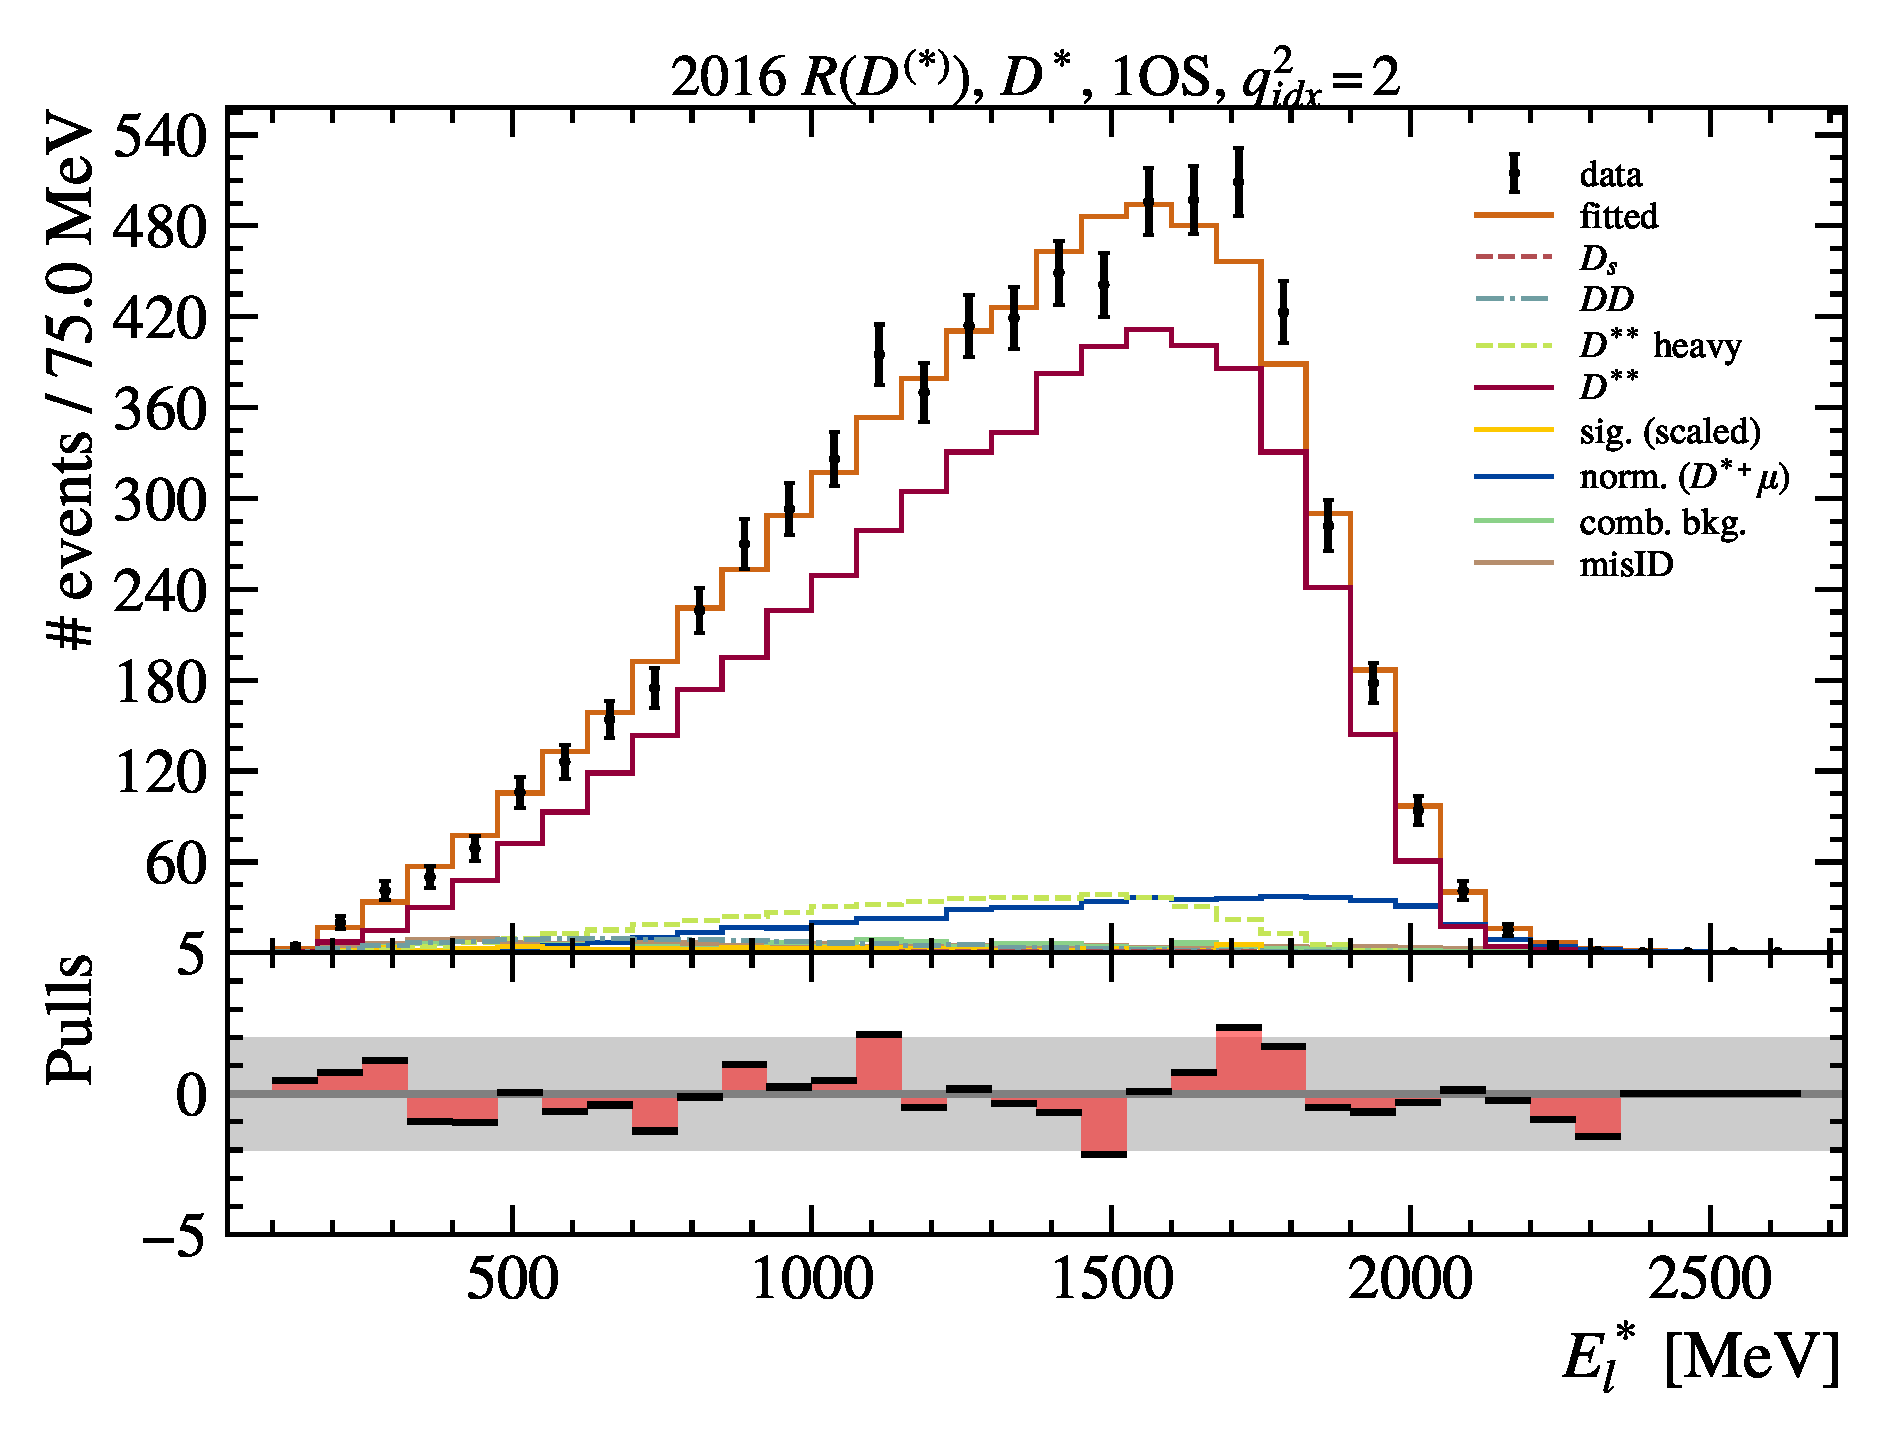
\includegraphics[width=0.24\textwidth]{./figs-fit-to-data/ctrl-fit/lines_q2_slices/fit_result-lines_q2_idx2-Dst-1os-el.pdf}
    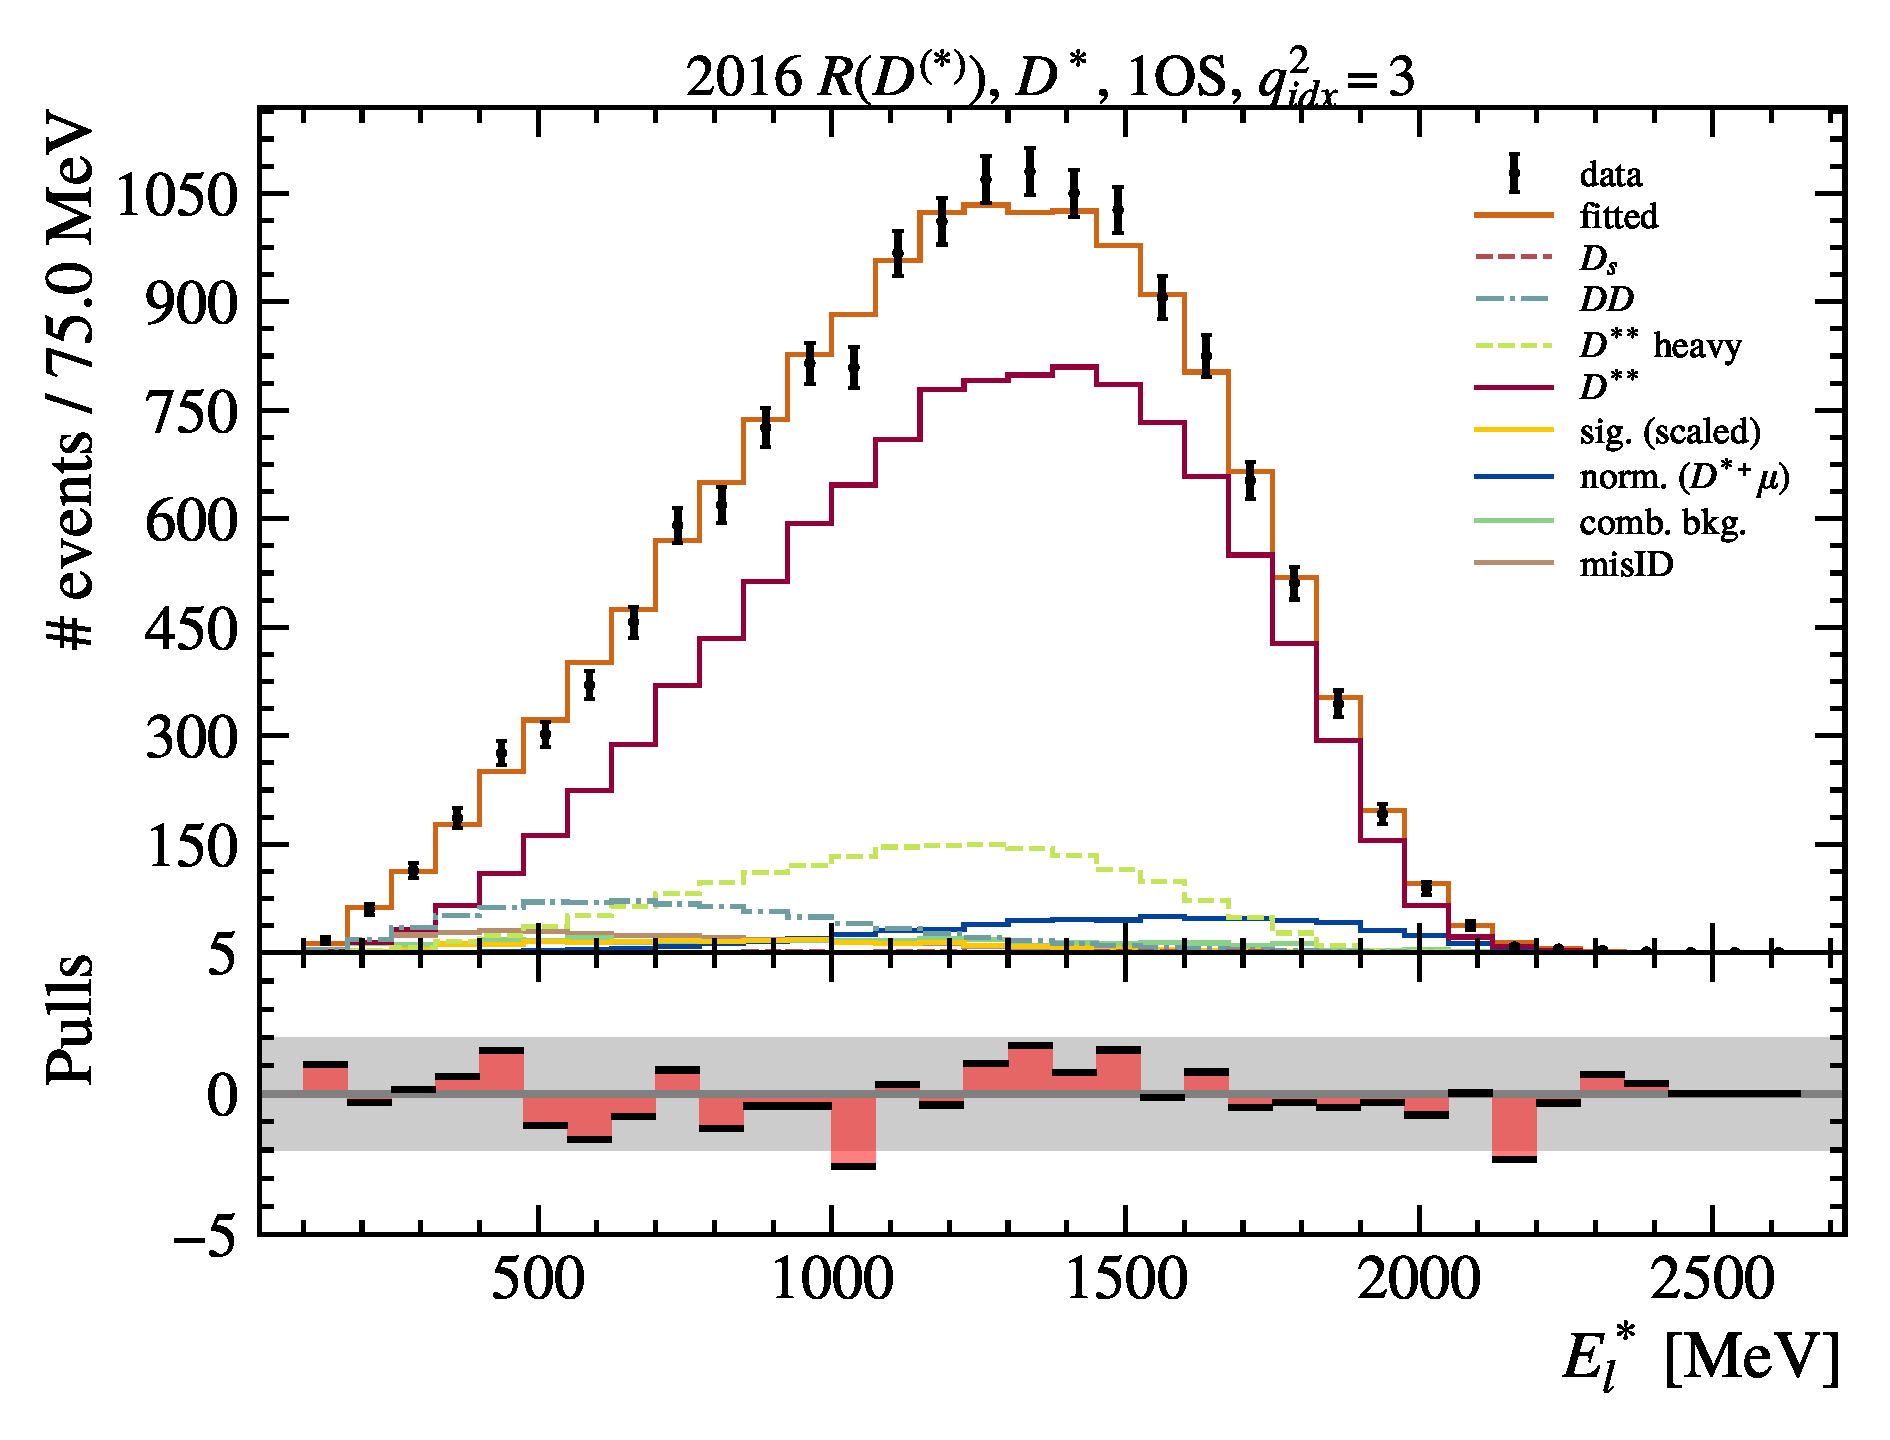
\includegraphics[width=0.24\textwidth]{./figs-fit-to-data/ctrl-fit/lines_q2_slices/fit_result-lines_q2_idx3-Dst-1os-el.pdf}
    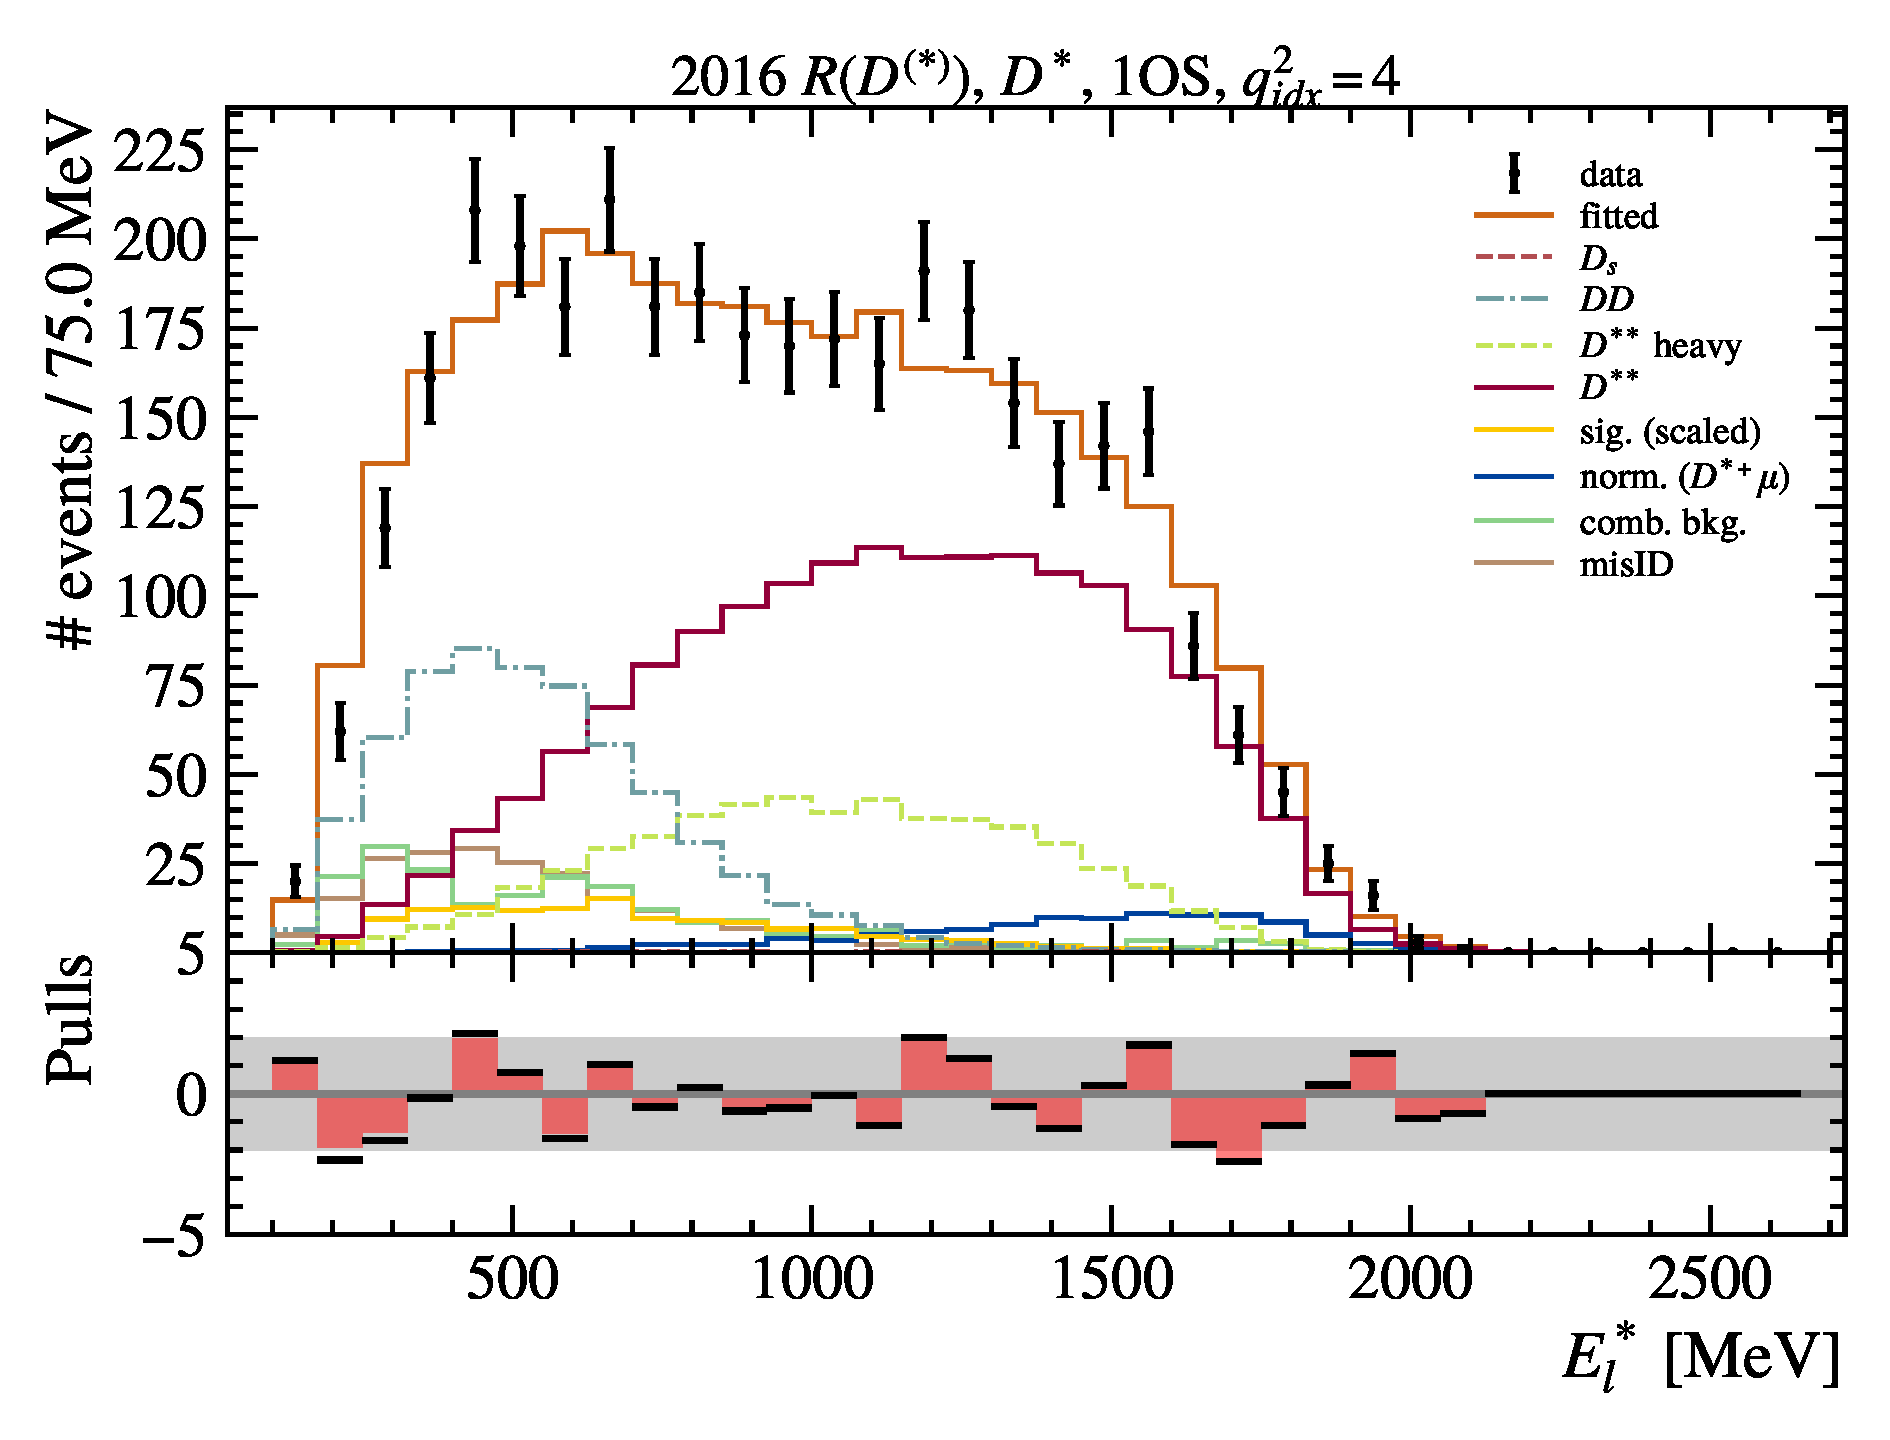
\includegraphics[width=0.24\textwidth]{./figs-fit-to-data/ctrl-fit/lines_q2_slices/fit_result-lines_q2_idx4-Dst-1os-el.pdf}

    \caption{Control fit for 1OS sample, \Dstar channel.}
    \label{fig:ctrl-1os-dst}
\end{figure}

\begin{figure}[htb]
    \centering
    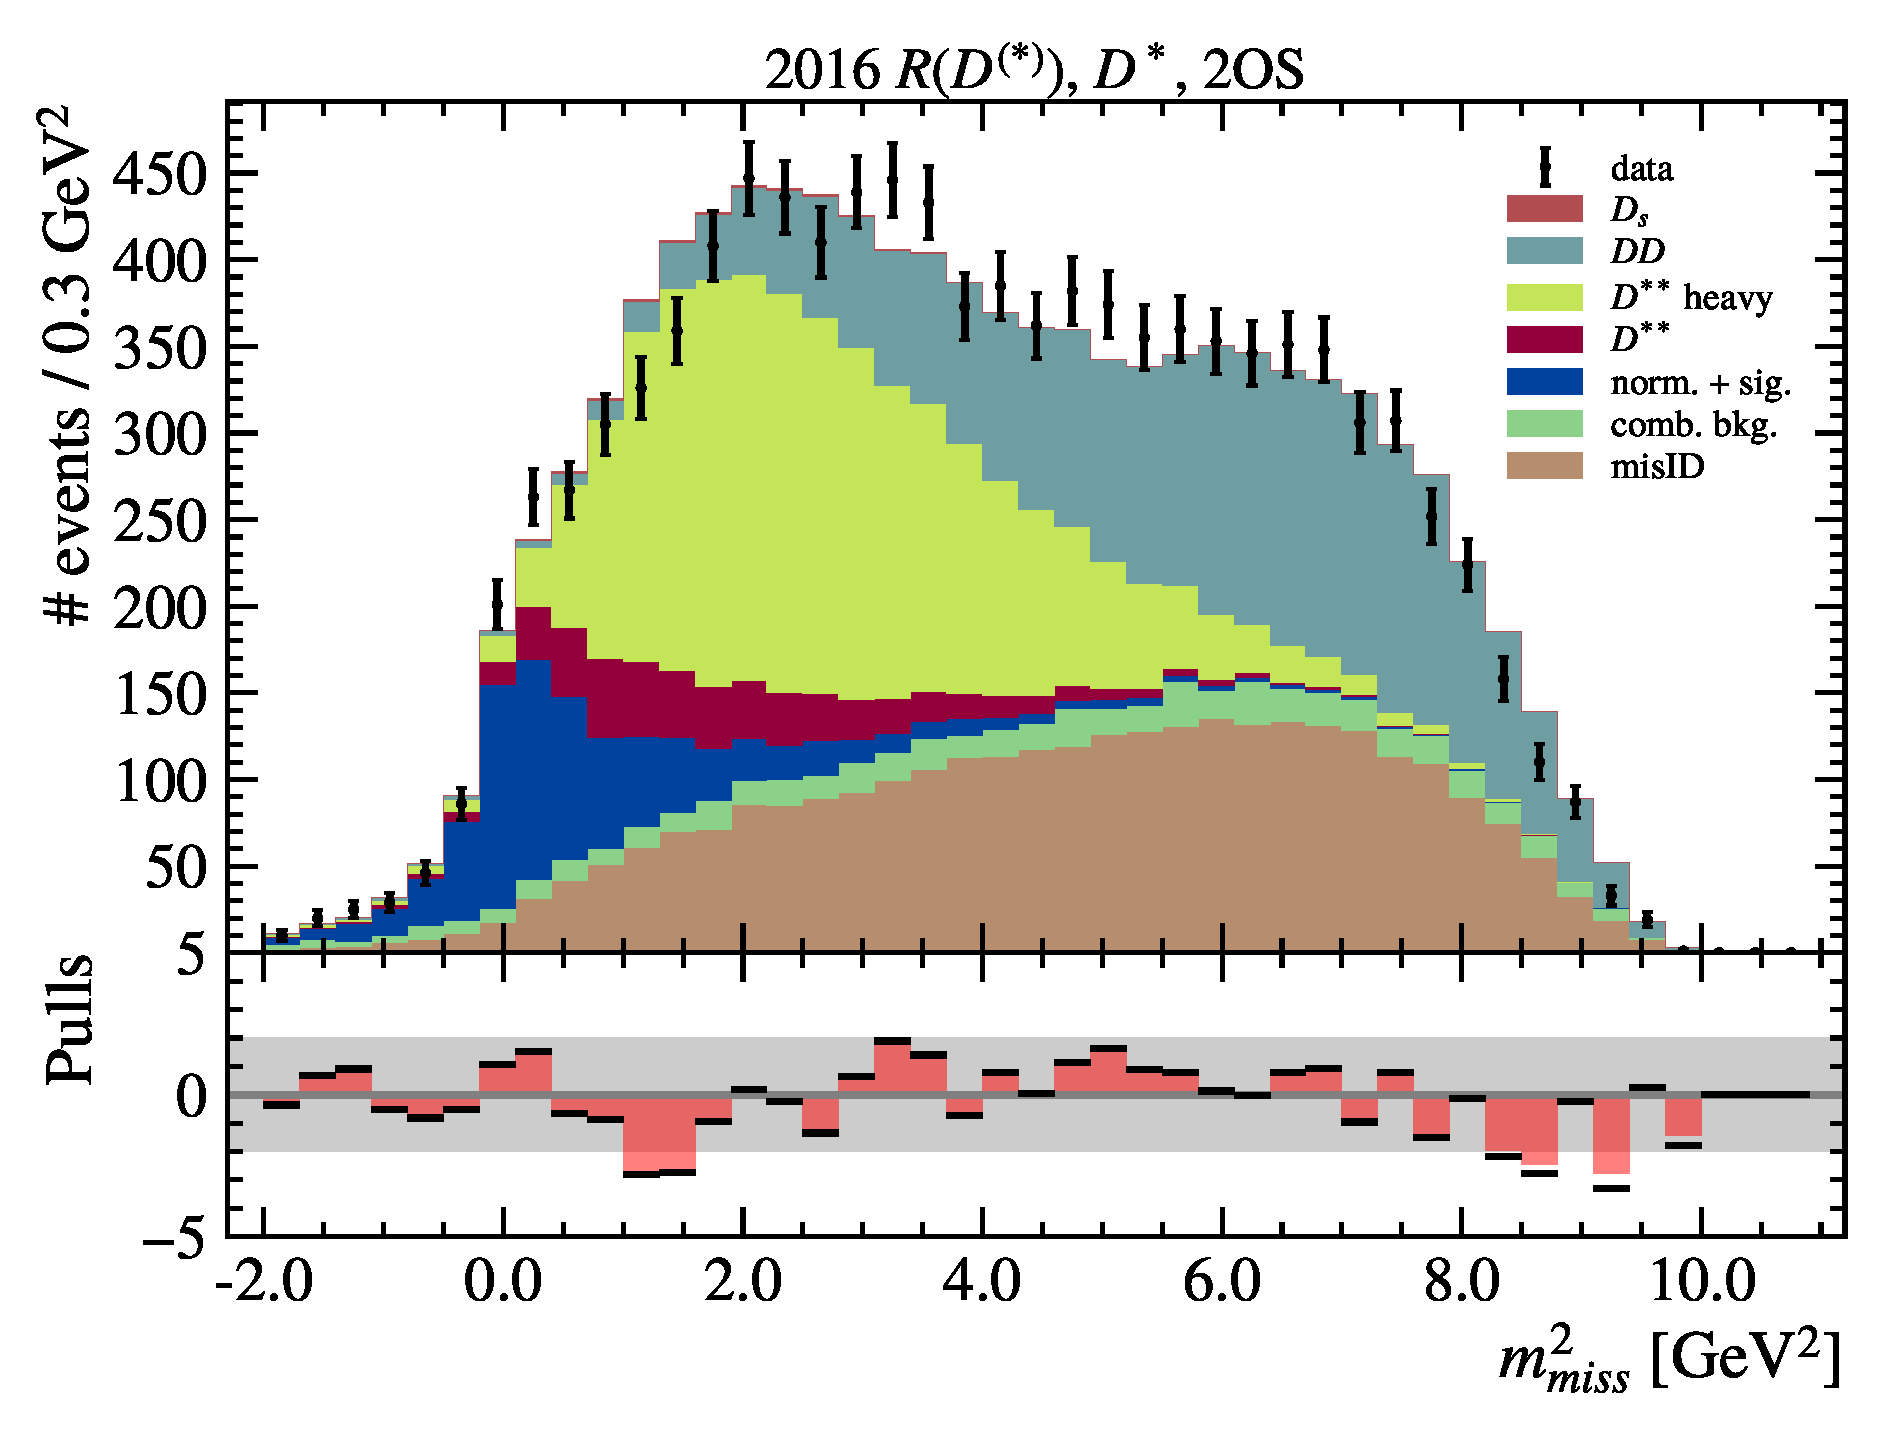
\includegraphics[width=0.32\textwidth]{./figs-fit-to-data/ctrl-fit/stacked/fit_result-stacked-Dst-2os-mmiss2.pdf}
    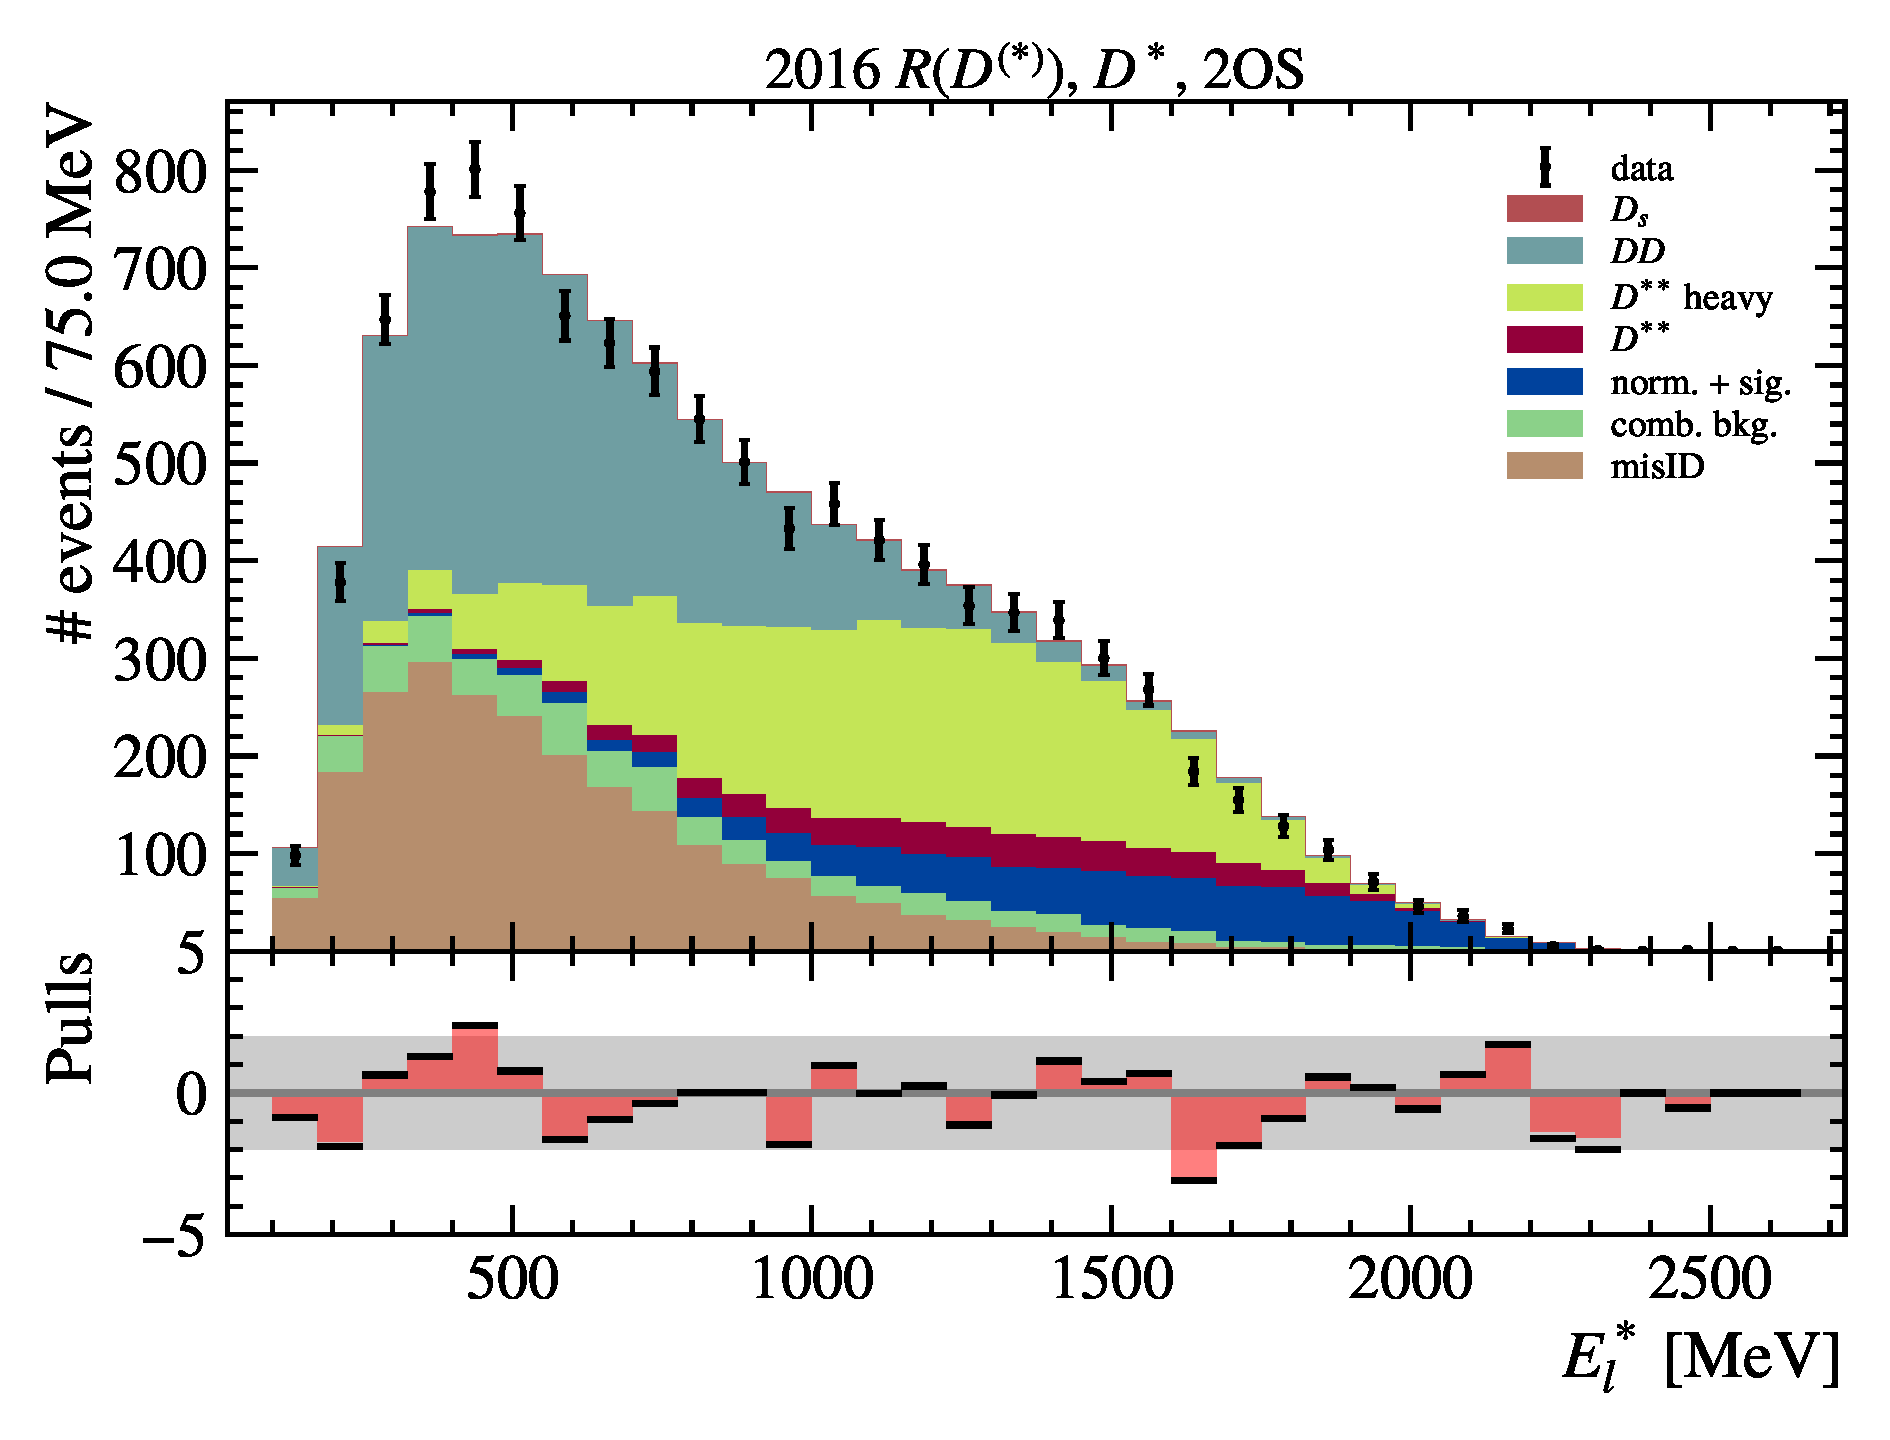
\includegraphics[width=0.32\textwidth]{./figs-fit-to-data/ctrl-fit/stacked/fit_result-stacked-Dst-2os-el.pdf}
    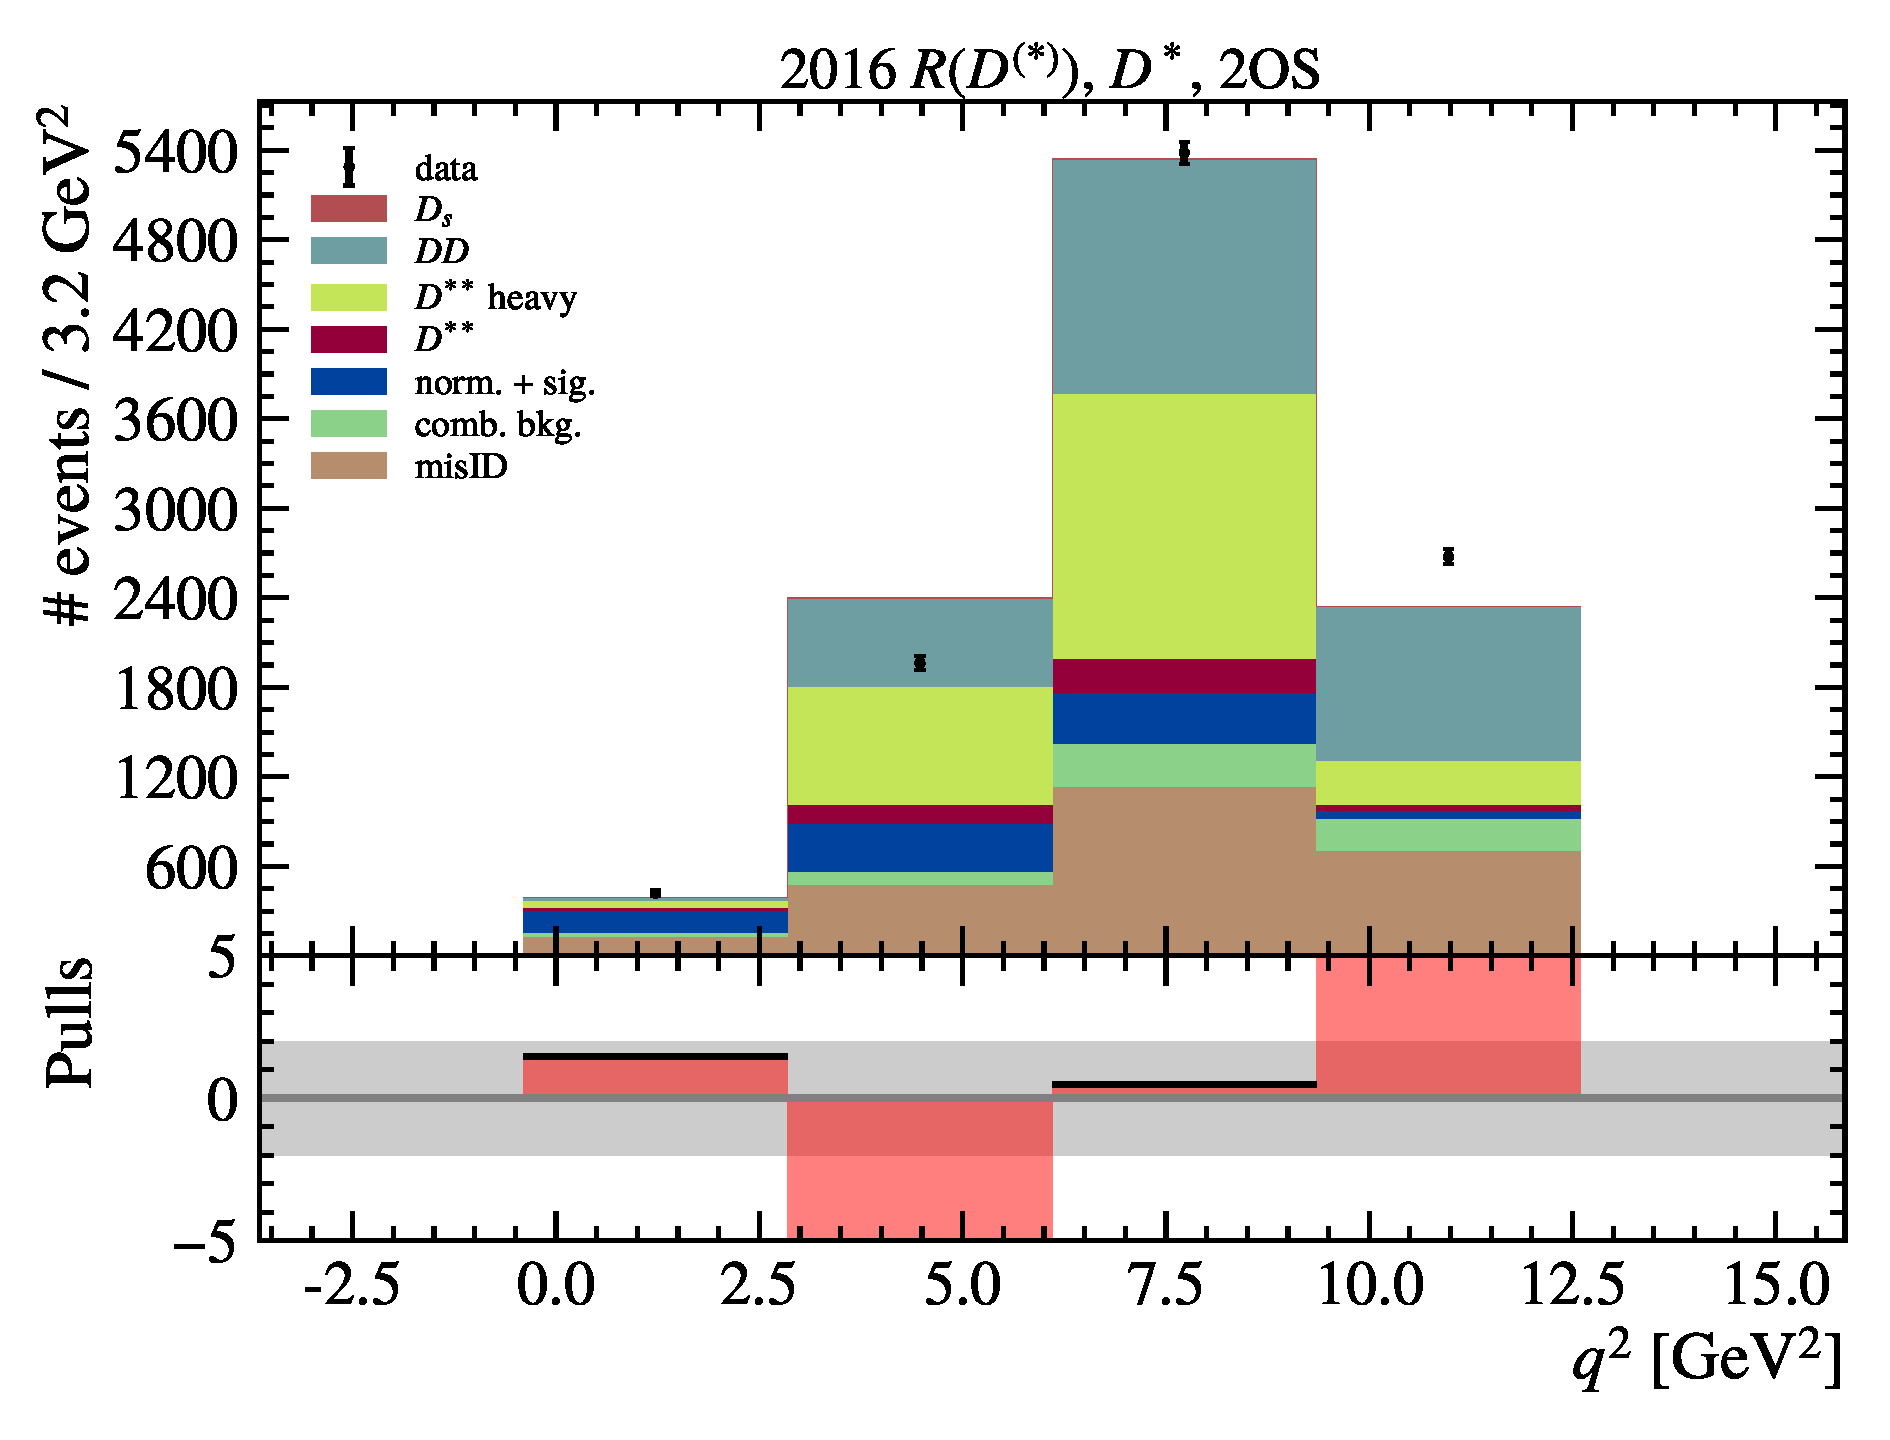
\includegraphics[width=0.32\textwidth]{./figs-fit-to-data/ctrl-fit/stacked/fit_result-stacked-Dst-2os-q2.pdf}

    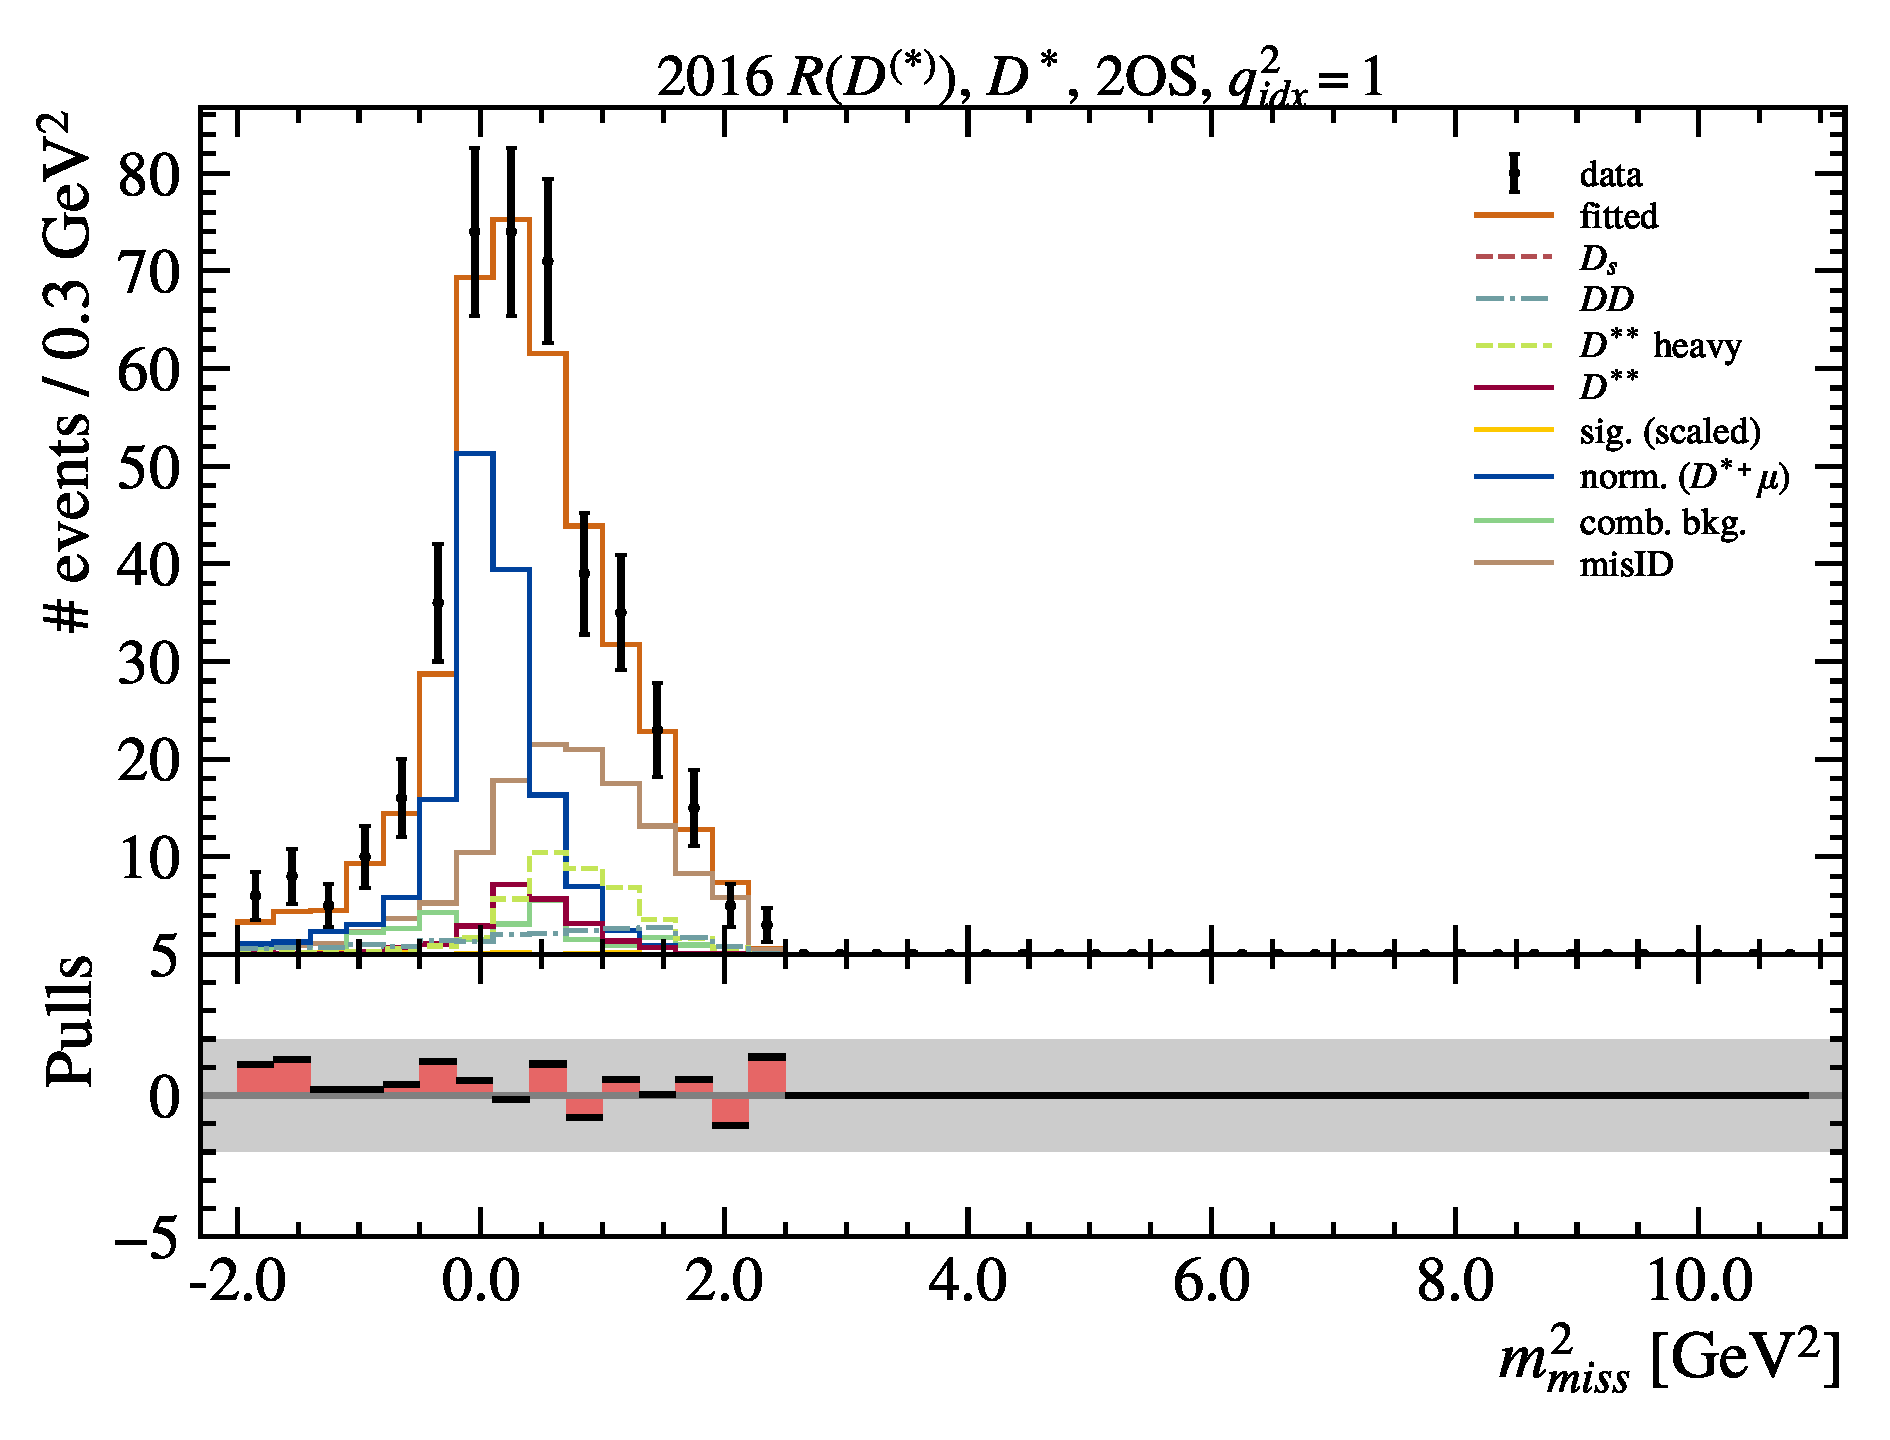
\includegraphics[width=0.24\textwidth]{./figs-fit-to-data/ctrl-fit/lines_q2_slices/fit_result-lines_q2_idx1-Dst-2os-mmiss2.pdf}
    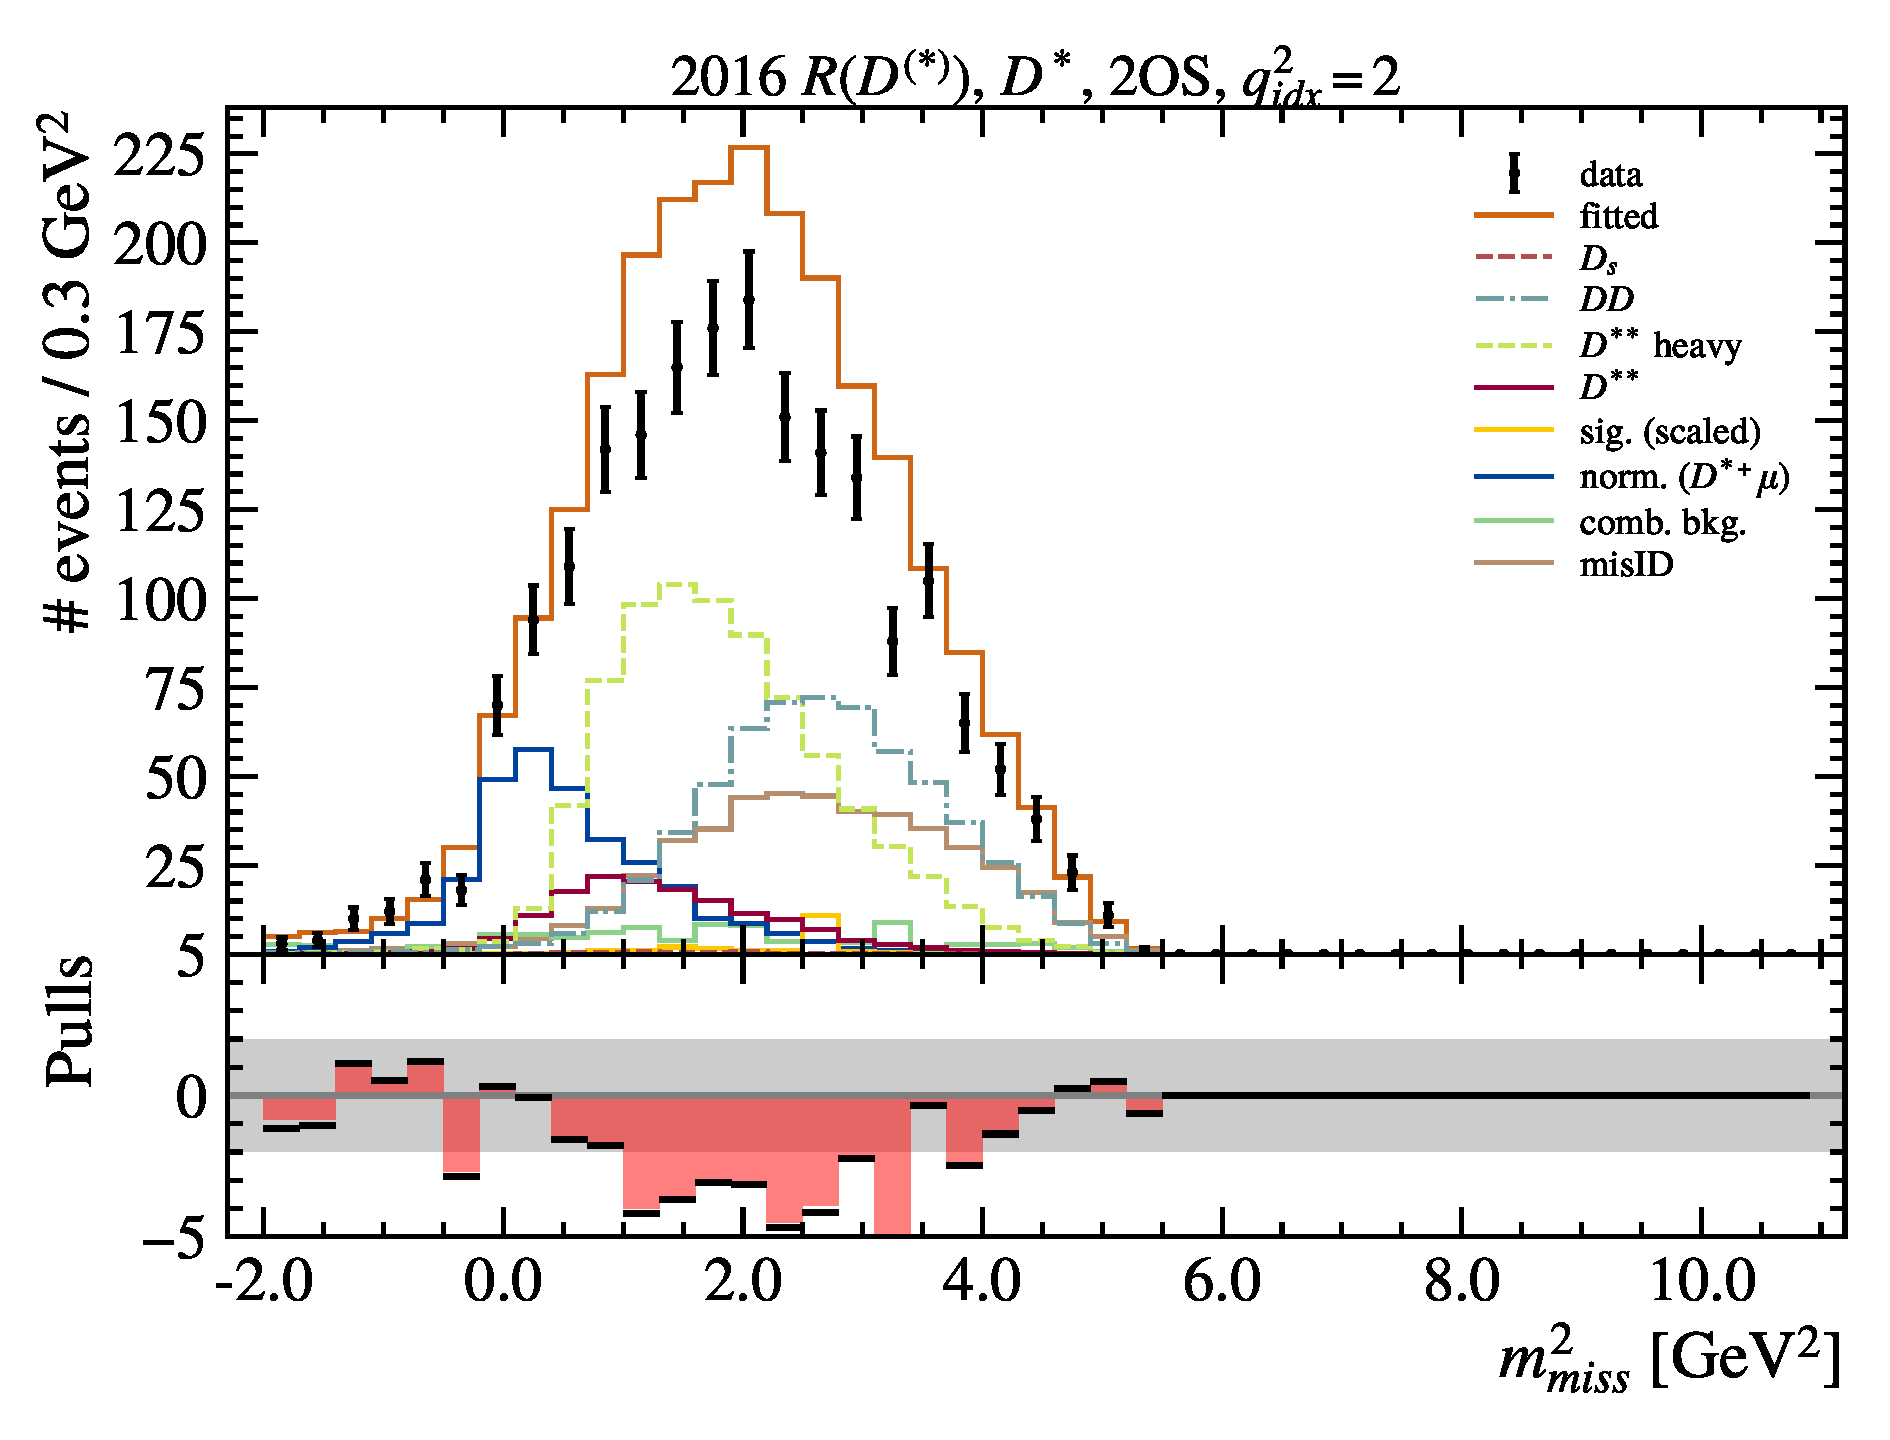
\includegraphics[width=0.24\textwidth]{./figs-fit-to-data/ctrl-fit/lines_q2_slices/fit_result-lines_q2_idx2-Dst-2os-mmiss2.pdf}
    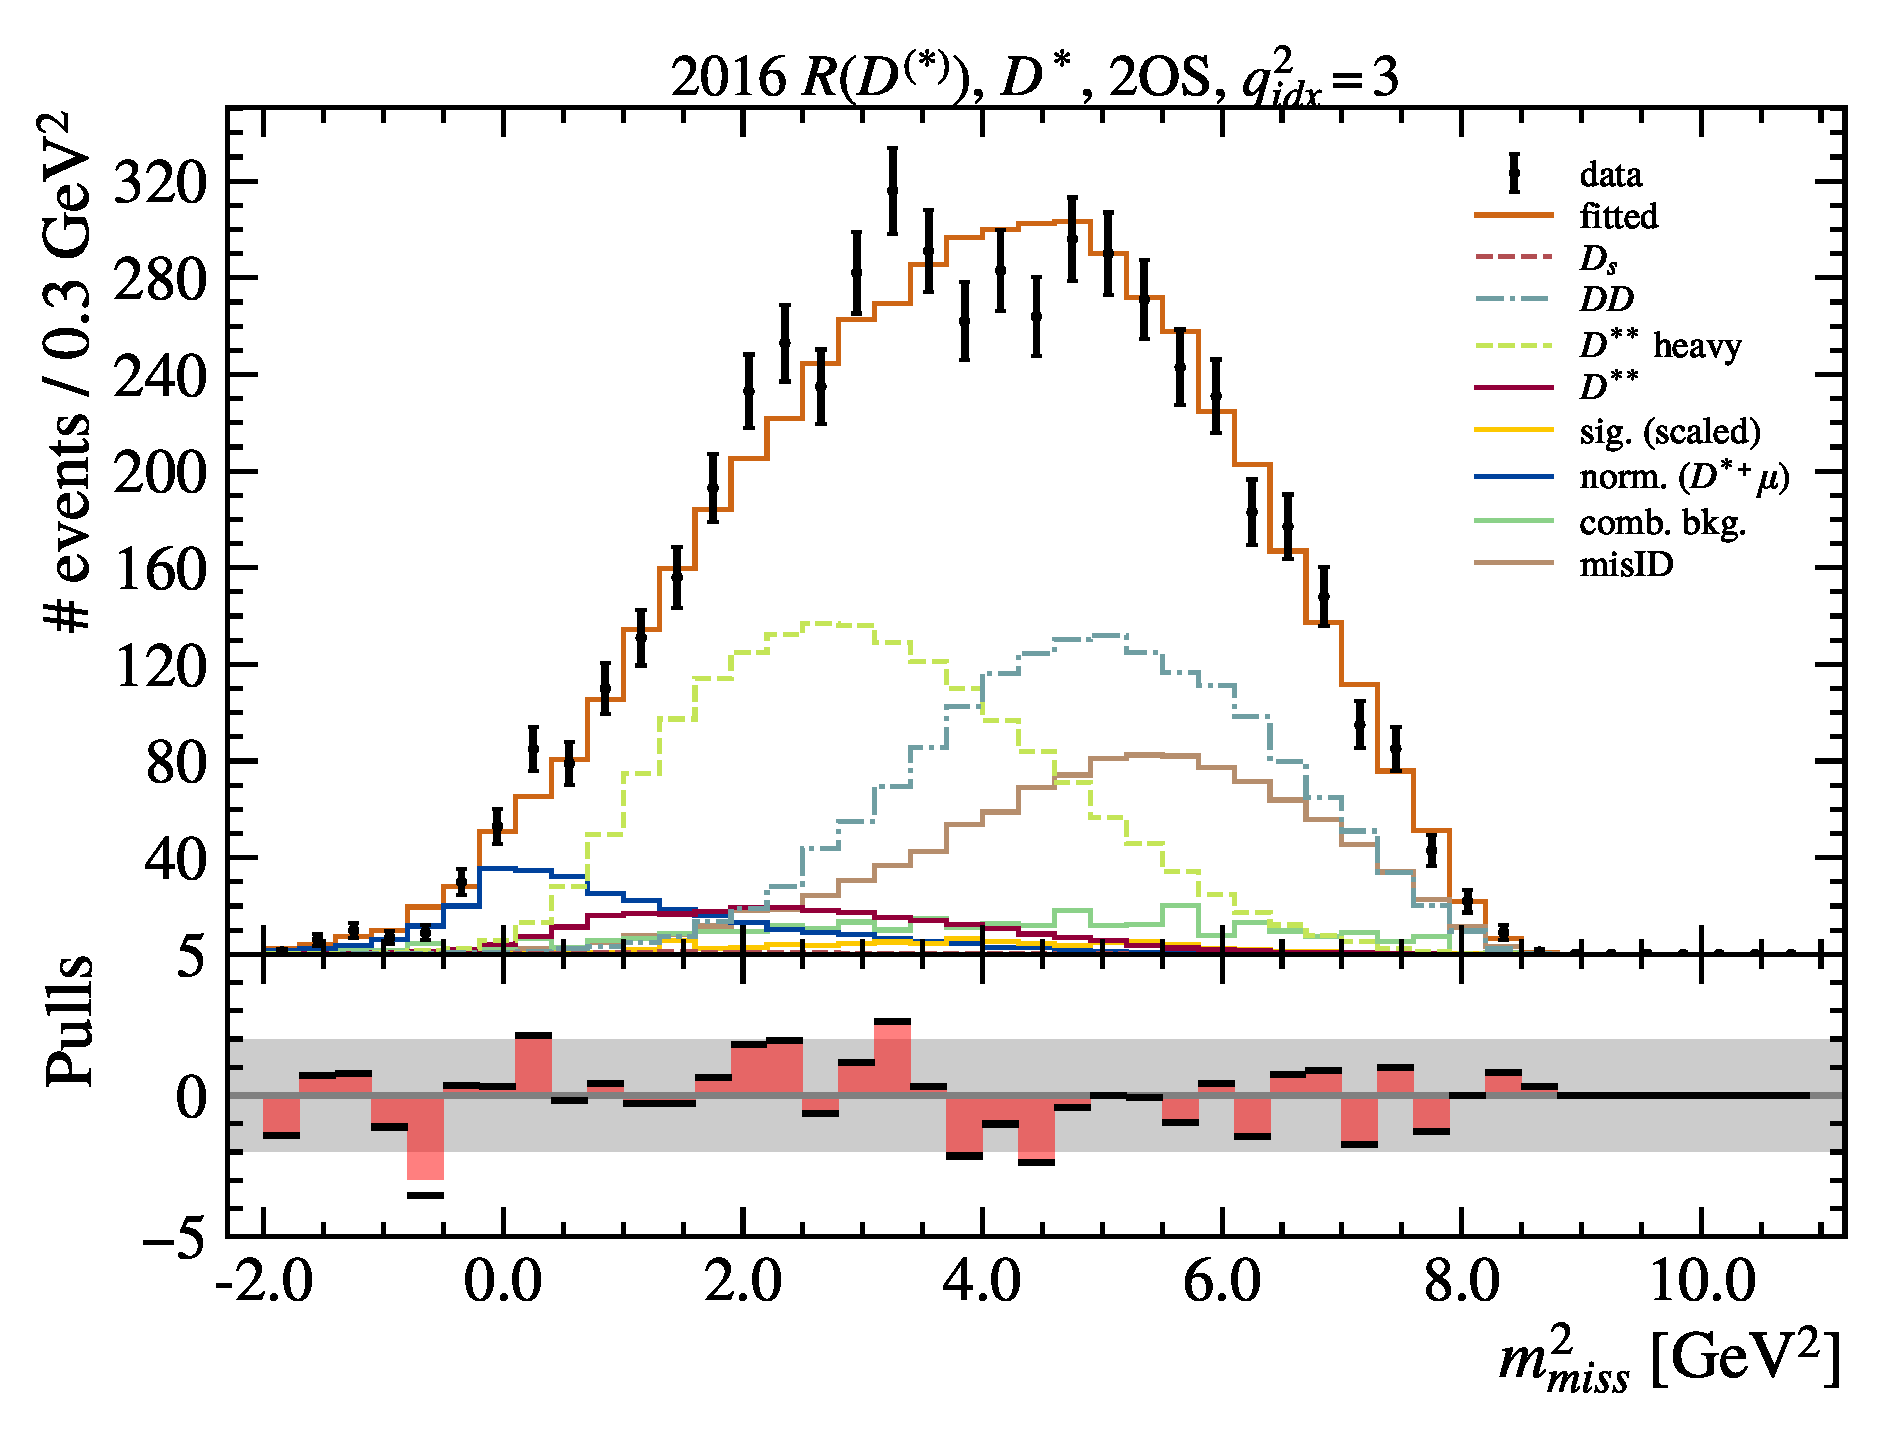
\includegraphics[width=0.24\textwidth]{./figs-fit-to-data/ctrl-fit/lines_q2_slices/fit_result-lines_q2_idx3-Dst-2os-mmiss2.pdf}
    \includegraphics[width=0.24\textwidth]{./figs-fit-to-data/ctrl-fit/lines_q2_slices/fit_result-lines_q2_idx4-Dst-2os-mmiss2.pdf}

    \includegraphics[width=0.24\textwidth]{./figs-fit-to-data/ctrl-fit/lines_q2_slices/fit_result-lines_q2_idx1-Dst-2os-el.pdf}
    \includegraphics[width=0.24\textwidth]{./figs-fit-to-data/ctrl-fit/lines_q2_slices/fit_result-lines_q2_idx2-Dst-2os-el.pdf}
    \includegraphics[width=0.24\textwidth]{./figs-fit-to-data/ctrl-fit/lines_q2_slices/fit_result-lines_q2_idx3-Dst-2os-el.pdf}
    \includegraphics[width=0.24\textwidth]{./figs-fit-to-data/ctrl-fit/lines_q2_slices/fit_result-lines_q2_idx4-Dst-2os-el.pdf}

    \caption{Control fit for 2OS sample, \Dstar channel.}
    \label{fig:ctrl-2os-dst}
\end{figure}

\begin{figure}[htb]
    \centering
    \includegraphics[width=0.32\textwidth]{./figs-fit-to-data/ctrl-fit/stacked/fit_result-stacked-Dst-dd-mmiss2.pdf}
    \includegraphics[width=0.32\textwidth]{./figs-fit-to-data/ctrl-fit/stacked/fit_result-stacked-Dst-dd-el.pdf}
    \includegraphics[width=0.32\textwidth]{./figs-fit-to-data/ctrl-fit/stacked/fit_result-stacked-Dst-dd-q2.pdf}

    \includegraphics[width=0.24\textwidth]{./figs-fit-to-data/ctrl-fit/lines_q2_slices/fit_result-lines_q2_idx1-Dst-dd-mmiss2.pdf}
    \includegraphics[width=0.24\textwidth]{./figs-fit-to-data/ctrl-fit/lines_q2_slices/fit_result-lines_q2_idx2-Dst-dd-mmiss2.pdf}
    \includegraphics[width=0.24\textwidth]{./figs-fit-to-data/ctrl-fit/lines_q2_slices/fit_result-lines_q2_idx3-Dst-dd-mmiss2.pdf}
    \includegraphics[width=0.24\textwidth]{./figs-fit-to-data/ctrl-fit/lines_q2_slices/fit_result-lines_q2_idx4-Dst-dd-mmiss2.pdf}

    \includegraphics[width=0.24\textwidth]{./figs-fit-to-data/ctrl-fit/lines_q2_slices/fit_result-lines_q2_idx1-Dst-dd-el.pdf}
    \includegraphics[width=0.24\textwidth]{./figs-fit-to-data/ctrl-fit/lines_q2_slices/fit_result-lines_q2_idx2-Dst-dd-el.pdf}
    \includegraphics[width=0.24\textwidth]{./figs-fit-to-data/ctrl-fit/lines_q2_slices/fit_result-lines_q2_idx3-Dst-dd-el.pdf}
    \includegraphics[width=0.24\textwidth]{./figs-fit-to-data/ctrl-fit/lines_q2_slices/fit_result-lines_q2_idx4-Dst-dd-el.pdf}

    \caption{Control fit for DD sample, \Dstar channel.}
    \label{fig:ctrl-dd-dst}
\end{figure}

\begin{figure}[htb]
    \centering
    \includegraphics[width=0.32\textwidth]{./figs-fit-to-data/sig-fit/stacked/fit_result-stacked-D0-iso-mmiss2.pdf}
    \includegraphics[width=0.32\textwidth]{./figs-fit-to-data/sig-fit/stacked/fit_result-stacked-D0-iso-el.pdf}
    \includegraphics[width=0.32\textwidth]{./figs-fit-to-data/sig-fit/stacked/fit_result-stacked-D0-iso-q2.pdf}

    \includegraphics[width=0.24\textwidth]{./figs-fit-to-data/sig-fit/lines_q2_slices/fit_result-lines_q2_idx1-D0-iso-mmiss2.pdf}
    \includegraphics[width=0.24\textwidth]{./figs-fit-to-data/sig-fit/lines_q2_slices/fit_result-lines_q2_idx2-D0-iso-mmiss2.pdf}
    \includegraphics[width=0.24\textwidth]{./figs-fit-to-data/sig-fit/lines_q2_slices/fit_result-lines_q2_idx3-D0-iso-mmiss2.pdf}
    \includegraphics[width=0.24\textwidth]{./figs-fit-to-data/sig-fit/lines_q2_slices/fit_result-lines_q2_idx4-D0-iso-mmiss2.pdf}

    \includegraphics[width=0.24\textwidth]{./figs-fit-to-data/sig-fit/lines_q2_slices/fit_result-lines_q2_idx1-D0-iso-el.pdf}
    \includegraphics[width=0.24\textwidth]{./figs-fit-to-data/sig-fit/lines_q2_slices/fit_result-lines_q2_idx2-D0-iso-el.pdf}
    \includegraphics[width=0.24\textwidth]{./figs-fit-to-data/sig-fit/lines_q2_slices/fit_result-lines_q2_idx3-D0-iso-el.pdf}
    \includegraphics[width=0.24\textwidth]{./figs-fit-to-data/sig-fit/lines_q2_slices/fit_result-lines_q2_idx4-D0-iso-el.pdf}

    \caption{Signal fit for ISO sample, \Dz channel.}
    \label{fig:sig-d0}
\end{figure}

\begin{figure}[htb]
    \centering
    \includegraphics[width=0.32\textwidth]{./figs-fit-to-data/sig-fit/stacked/fit_result-stacked-Dst-iso-mmiss2.pdf}
    \includegraphics[width=0.32\textwidth]{./figs-fit-to-data/sig-fit/stacked/fit_result-stacked-Dst-iso-el.pdf}
    \includegraphics[width=0.32\textwidth]{./figs-fit-to-data/sig-fit/stacked/fit_result-stacked-Dst-iso-q2.pdf}

    \includegraphics[width=0.24\textwidth]{./figs-fit-to-data/sig-fit/lines_q2_slices/fit_result-lines_q2_idx1-Dst-iso-mmiss2.pdf}
    \includegraphics[width=0.24\textwidth]{./figs-fit-to-data/sig-fit/lines_q2_slices/fit_result-lines_q2_idx2-Dst-iso-mmiss2.pdf}
    \includegraphics[width=0.24\textwidth]{./figs-fit-to-data/sig-fit/lines_q2_slices/fit_result-lines_q2_idx3-Dst-iso-mmiss2.pdf}
    \includegraphics[width=0.24\textwidth]{./figs-fit-to-data/sig-fit/lines_q2_slices/fit_result-lines_q2_idx4-Dst-iso-mmiss2.pdf}

    \includegraphics[width=0.24\textwidth]{./figs-fit-to-data/sig-fit/lines_q2_slices/fit_result-lines_q2_idx1-Dst-iso-el.pdf}
    \includegraphics[width=0.24\textwidth]{./figs-fit-to-data/sig-fit/lines_q2_slices/fit_result-lines_q2_idx2-Dst-iso-el.pdf}
    \includegraphics[width=0.24\textwidth]{./figs-fit-to-data/sig-fit/lines_q2_slices/fit_result-lines_q2_idx3-Dst-iso-el.pdf}
    \includegraphics[width=0.24\textwidth]{./figs-fit-to-data/sig-fit/lines_q2_slices/fit_result-lines_q2_idx4-Dst-iso-el.pdf}

    \caption{Signal fit for ISO sample, \Dstar channel.}
    \label{fig:sig-dst}
\end{figure}


\begin{table}[htb]
    \centering
    \caption{Index for selected fit parameters.}
    \label{tab:selected-fit-params}
    \begin{tabular}{r|l|l}
        \toprule
        {\bf Parameter(s)} & {\bf Utility} & {\bf Reference} \\
        \midrule
        $N_{D\mu}$, $N_{\Dstar\mu}$    & overall norm.  & \cref{tmpl:sig-norm} \\
        \RD, \RDstp, \RDstz & frac. of signal to related norm. &  \\
        \midrule
        $n^{0}_{D^{**}},f^{*}_{D^{**}}$ & mental aid & \cref{tmpl:dstst} \\
        \bottomrule
    \end{tabular}
\end{table}
